\documentclass[review]{elsarticle}

\usepackage{lineno}
\usepackage{xspace}
\modulolinenumbers[5]

\journal{Annals of Nuclear Energy}

%% `Elsevier LaTeX' style
\bibliographystyle{elsarticle-num}
%%%%%%%%%%%%%%%%%%%%%%%

%%%% packages and definitions (optional)
\usepackage{placeins}
\usepackage{booktabs} % nice rules (thick lines) for tables
\usepackage{microtype} % improves typography for PDF
\usepackage{hhline}
\usepackage{amsmath}
\usepackage{enumitem}
%\usepackage[demo]{graphicx}
%\usepackage{caption}
%\usepackage{subcaption}

\usepackage{booktabs}
\usepackage{threeparttable, tablefootnote}

\usepackage{tabularx}
\newcolumntype{b}{>{\hsize=1.0\hsize}X}
\newcolumntype{s}{>{\hsize=.5\hsize}X}
\newcolumntype{m}{>{\hsize=.75\hsize}X}
\newcolumntype{x}{>{\hsize=.25\hsize}X}
\newcolumntype{L}{>{\raggedright\arraybackslash}X}
\newcolumntype{R}{>{\raggedleft\arraybackslash}X}

\graphicspath{{../dissertation/figures/}}

% tikz %
\usepackage{tikz}
\usetikzlibrary{positioning, arrows, decorations, shapes}

\usetikzlibrary{shapes.geometric,arrows}
\tikzstyle{process} = [rectangle, rounded corners, minimum width=3cm, minimum height=1cm,text centered, draw=black, fill=blue!30]
\tikzstyle{object} = [ellipse, rounded corners, minimum width=3cm, minimum height=1cm,text centered, draw=black, fill=green!30]
\tikzstyle{arrow} = [thick,->,>=stealth]

% hyperref %
\usepackage[hidelinks]{hyperref}
% after hyperref %
\usepackage{cleveref}
\usepackage{datatool}
\usepackage[acronym,toc]{glossaries}
%\newacronym{<++>}{<++>}{<++>}
\newacronym[longplural={metric tons of heavy metal}]{MTHM}{MTHM}{metric ton of heavy metal}
\newacronym{ABM}{ABM}{agent-based modeling}
\newacronym{ACDIS}{ACDIS}{Program in Arms Control \& Domestic and International Security}
\newacronym{AHTR}{AHTR}{Advanced High Temperature Reactor}
\newacronym{ANDRA}{ANDRA}{Agence Nationale pour la gestion des D\'echets RAdioactifs, the French National Agency for Radioactive Waste Management}
\newacronym{ANL}{ANL}{Argonne National Laboratory}
\newacronym{ANS}{ANS}{American Nuclear Society}
\newacronym{AOA}{AOA}{Axial Offset Anomaly}
\newacronym{API}{API}{application programming interface}
\newacronym{ARE}{ARE}{Aircraft Reactor Experiment}
\newacronym{ARFC}{ARFC}{Advanced Reactors and Fuel Cycles}
\newacronym{ASME}{ASME}{American Society of Mechanical Engineers}
\newacronym{ATWS}{ATWS}{Anticipated Transient Without Scram}
\newacronym{BOC}{BOC}{Beginning of Cycle}
\newacronym{BOL}{BOL}{Beginning of Life}
\newacronym{BDBE}{BDBE}{Beyond Design Basis Event}
\newacronym{BIDS}{BIDS}{Berkeley Institute for Data Science}
\newacronym{BWR}{BWR}{Boiling Water Reactor}
\newacronym{CAFCA}{CAFCA}{ Code for Advanced Fuel Cycles Assessment }
\newacronym{CDTN}{CDTN}{Centro de Desenvolvimento da Tecnologia Nuclear}
\newacronym{CFD}{CFD}{Computational Fluid Dynamics}
\newacronym{CEA}{CEA}{Commissariat \`a l'\'Energie Atomique et aux \'Energies Alternatives}
\newacronym{CI}{CI}{continuous integration}
\newacronym{CNEN}{CNEN}{Comiss\~{a}o Nacional de Energia Nuclear}
\newacronym{CNERG}{CNERG}{Computational Nuclear Engineering Research Group}
\newacronym{COSI}{COSI}{Commelini-Sicard}
\newacronym{COTS}{COTS}{commercial, off-the-shelf}
\newacronym{CSNF}{CSNF}{commercial spent nuclear fuel}
\newacronym{CTAH}{CTAHs}{Coiled Tube Air Heaters}
\newacronym{CUBIT}{CUBIT}{CUBIT Geometry and Mesh Generation Toolkit}
\newacronym{CURIE}{CURIE}{Centralized Used Fuel Resource for Information Exchange}
\newacronym{CR}{CR}{conversion ratio}
\newacronym{DAG}{DAG}{directed acyclic graph}
\newacronym{DANESS}{DANESS}{Dynamic Analysis of Nuclear Energy System Strategies}
\newacronym{DBE}{DBE}{Design Basis Event}
\newacronym{DESAE}{DESAE}{Dynamic Analysis of Nuclear Energy Systems Strategies}
\newacronym{DHS}{DHS}{Department of Homeland Security}
\newacronym{DOE}{DOE}{Department of Energy}
\newacronym{DRACS}{DRACS}{Direct Reactor Auxiliary Cooling System}
\newacronym{DRE}{DRE}{dynamic resource exchange}
\newacronym{DSNF}{DSNF}{DOE spent nuclear fuel}
\newacronym{DYMOND}{DYMOND}{Dynamic Model of Nuclear Development }
\newacronym{EBS}{EBS}{Engineered Barrier System}
\newacronym{EDF}{EDF}{Électricité de France}
\newacronym{EDZ}{EDZ}{Excavation Disturbed Zone}
\newacronym{EOC}{EOC}{End of Cycle}
\newacronym{EOL}{EOL}{End of Life}
\newacronym{EIA}{EIA}{U.S. Energy Information Administration}
\newacronym{EPA}{EPA}{Environmental Protection Agency}
\newacronym{EPR}{EPR}{European Pressurized Reactors}
\newacronym{EP}{EP}{Engineering Physics}
\newacronym{EU}{EU}{European Union}
\newacronym{FCO}{FCO}{Fuel Cycle Options}
\newacronym{FCT}{FCT}{Fuel Cycle Technology}
\newacronym{FEHM}{FEHM}{Finite Element Heat and Mass Transfer}
\newacronym{FEPs}{FEPs}{Features, Events, and Processes}
\newacronym{FHR}{FHR}{Fluoride-Salt-Cooled High-Temperature Reactor}
\newacronym{FLiBe}{FLiBe}{Fluoride-Lithium-Beryllium}
\newacronym{FP}{FP}{Fission Product}
\newacronym{FTC}{FTC}{fuel temperature coefficient}
\newacronym{GDSE}{GDSE}{Generic Disposal System Environment}
\newacronym{GDSM}{GDSM}{Generic Disposal System Model}
\newacronym{GENIUSv1}{GENIUSv1}{Global Evaluation of Nuclear Infrastructure Utilization Scenarios, Version 1}
\newacronym{GENIUSv2}{GENIUSv2}{Global Evaluation of Nuclear Infrastructure Utilization Scenarios, Version 2}
\newacronym{GENIUS}{GENIUS}{Global Evaluation of Nuclear Infrastructure Utilization Scenarios}
\newacronym{GPAM}{GPAM}{Generic Performance Assessment Model}
\newacronym{GRSAC}{GRSAC}{Graphite Reactor Severe Accident Code}
\newacronym{GUI}{GUI}{graphical user interface}
\newacronym{HFP}{HFP}{hot full power}
\newacronym{HLW}{HLW}{high level waste}
\newacronym{HPC}{HPC}{high-performance computing}
\newacronym{HTC}{HTC}{high-throughput computing}
\newacronym{HTGR}{HTGR}{High Temperature Gas-Cooled Reactor}
\newacronym{HZP}{HZP}{hot zero power}
\newacronym{IAEA}{IAEA}{International Atomic Energy Agency}
\newacronym{IEMA}{IEMA}{Illinois Emergency Mangament Agency}
\newacronym{IHLRWM}{IHLRWM}{International High Level Radioactive Waste Management}
\newacronym{INL}{INL}{Idaho National Laboratory}
\newacronym{IPRR1}{IRP-R1}{Instituto de Pesquisas Radioativas Reator 1}
\newacronym{IRP}{IRP}{Integrated Research Project}
\newacronym{ISFSI}{ISFSI}{Independent Spent Fuel Storage Installation}
\newacronym{ISRG}{ISRG}{Independent Student Research Group}
\newacronym{JFNK}{JFNK}{Jacobian-Free Newton Krylov}
\newacronym{LANL}{LANL}{Los Alamos National Laboratory}
\newacronym{LBNL}{LBNL}{Lawrence Berkeley National Laboratory}
\newacronym{LCOE}{LCOE}{levelized cost of electricity}
\newacronym{LEU}{LEU}{low-enriched uranium}
\newacronym{LDRD}{LDRD}{laboratory directed research and development}
\newacronym{LFR}{LFR}{Lead-Cooled Fast Reactor}
\newacronym{LLNL}{LLNL}{Lawrence Livermore National Laboratory}
\newacronym{LMFBR}{LMFBR}{Liquid Metal Fast Breeder Reactor}
\newacronym{LOFC}{LOFC}{Loss of Forced Cooling}
\newacronym{LOHS}{LOHS}{Loss of Heat Sink}
\newacronym{LOLA}{LOLA}{Loss of Large Area}
\newacronym{LP}{LP}{linear program}
\newacronym{LWR}{LWR}{Light Water Reactor}
\newacronym{MAGNOX}{MAGNOX}{Magnesium Alloy Graphie Moderated Gas Cooled Uranium Oxide Reactor}
\newacronym{MA}{MA}{minor actinide}
\newacronym{MCNP}{MCNP}{Monte Carlo N-Particle code}
\newacronym{MILP}{MILP}{mixed-integer linear program}
\newacronym{MIT}{MIT}{the Massachusetts Institute of Technology}
\newacronym{MOAB}{MOAB}{Mesh-Oriented datABase}
\newacronym{MOOSE}{MOOSE}{Multiphysics Object-Oriented Simulation Environment}
\newacronym{MOSART}{MOSART}{Molten Salt Actinide Recycler and Transmuter}
\newacronym{MOX}{MOX}{mixed oxide}
\newacronym{MPI}{MPI}{Message Passing Interface}
\newacronym{MSBR}{MSBR}{Molten Salt Breeder Reactor}
\newacronym{MSFR}{MSFR}{Molten Salt Fast Reactor}
\newacronym{MSRE}{MSRE}{Molten Salt Reactor Experiment}
\newacronym{MSR}{MSR}{Molten Salt Reactor}
\newacronym{MTC}{MTC}{moderator temperature coefficient}
\newacronym{NAGRA}{NAGRA}{National Cooperative for the Disposal of Radioactive Waste}
\newacronym{NEAMS}{NEAMS}{Nuclear Engineering Advanced Modeling and Simulation}
\newacronym{NEUP}{NEUP}{Nuclear Energy University Programs}
\newacronym{NFCSim}{NFCSim}{Nuclear Fuel Cycle Simulator}
\newacronym{NGNP}{NGNP}{Next Generation Nuclear Plant}
\newacronym{NMWPC}{NMWPC}{Nuclear MW Per Capita}
\newacronym{NNSA}{NNSA}{National Nuclear Security Administration}
\newacronym{NPP}{NPP}{Nuclear Power Plant}
\newacronym{NPRE}{NPRE}{Department of Nuclear, Plasma, and Radiological Engineering}
\newacronym{NQA1}{NQA-1}{Nuclear Quality Assurance - 1}
\newacronym{NRC}{NRC}{Nuclear Regulatory Commission}
\newacronym{NSF}{NSF}{National Science Foundation}
\newacronym{NSSC}{NSSC}{Nuclear Science and Security Consortium}
\newacronym{NUWASTE}{NUWASTE}{Nuclear Waste Assessment System for Technical Evaluation}
\newacronym{NWF}{NWF}{Nuclear Waste Fund}
\newacronym{NWTRB}{NWTRB}{Nuclear Waste Technical Review Board}
\newacronym{OCRWM}{OCRWM}{Office of Civilian Radioactive Waste Management}
\newacronym{OOP}{OOP}{Object-Oriented Programming}
\newacronym{ORION}{ORION}{ORION}
\newacronym{ORNL}{ORNL}{Oak Ridge National Laboratory}
\newacronym{PARCS}{PARCS}{Purdue Advanced Reactor Core Simulator}
\newacronym{PBAHTR}{PB-AHTR}{Pebble Bed Advanced High Temperature Reactor}
\newacronym{PBFHR}{PB-FHR}{Pebble-Bed Fluoride-Salt-Cooled High-Temperature Reactor}
\newacronym{PEI}{PEI}{Peak Environmental Impact}
\newacronym{PH}{PRONGHORN}{PRONGHORN}
\newacronym{PRIS}{PRIS}{Power Reactor Information System}
\newacronym{PRKE}{PRKE}{Point Reactor Kinetics Equations}
\newacronym{PSPG}{PSPG}{Pressure-Stabilizing/Petrov-Galerkin}
\newacronym{PWAR}{PWAR}{Pratt and Whitney Aircraft Reactor}
\newacronym{PWR}{PWR}{Pressurized Water Reactor}
\newacronym{PyNE}{PyNE}{Python toolkit for Nuclear Engineering}
\newacronym{PyRK}{PyRK}{Python for Reactor Kinetics}
\newacronym{QA}{QA}{quality assurance}
\newacronym{RDD}{RD\&D}{Research Development and Demonstration}
\newacronym{RD}{R\&D}{Research and Development}
\newacronym{REE}{REE}{rare earth element}
\newacronym{RELAP}{RELAP}{Reactor Excursion and Leak Analysis Program}
\newacronym{REM}{REM}{Rules for Evolution calculations with MCNP}
\newacronym{RIA}{RIA}{Reactivity Insertion Accident}
\newacronym{RIF}{RIF}{Region-Institution-Facility}
\newacronym{SFR}{SFR}{Sodium-Cooled Fast Reactor}
\newacronym{SINDAG}{SINDA{\textbackslash}G}{Systems Improved Numerical Differencing Analyzer $\backslash$ Gaski}
\newacronym{SKB}{SKB}{Svensk K\"{a}rnbr\"{a}nslehantering AB}
\newacronym{SNF}{SNF}{spent nuclear fuel}
\newacronym{SNL}{SNL}{Sandia National Laboratory}
\newacronym{STC}{STC}{specific temperature change}
\newacronym{SUPG}{SUPG}{Streamline-Upwind/Petrov-Galerkin}
\newacronym{SVF}{SVF}{salt volume fraction}
\newacronym{SWF}{SWF}{Separations and Waste Forms}
\newacronym{SWU}{SWU}{Separative Work Unit}
\newacronym{TAP}{TAP}{Transatomic Power}
\newacronym{TRIGA}{TRIGA}{Training Research Isotope General Atomic}
\newacronym{TRISO}{TRISO}{Tristructural Isotropic}
\newacronym{TSM}{TSM}{Total System Model}
\newacronym{TSPA}{TSPA}{Total System Performance Assessment for the Yucca Mountain License Application}
\newacronym{ThOX}{ThOX}{thorium oxide}
\newacronym{UFD}{UFD}{Used Fuel Disposition}
\newacronym{UML}{UML}{Unified Modeling Language}
\newacronym{UOX}{UOX}{uranium oxide}
\newacronym{UQ}{UQ}{uncertainty quantification}
\newacronym{US}{US}{United States}
\newacronym{UW}{UW}{University of Wisconsin}
\newacronym{VISION}{VISION}{the Verifiable Fuel Cycle Simulation Model}
\newacronym{VVER}{VVER}{Voda-Vodyanoi Energetichesky Reaktor (Russian Pressurized Water Reactor)}
\newacronym{VV}{V\&V}{verification and validation}
\newacronym{WIPP}{WIPP}{Waste Isolation Pilot Plant}
\newacronym{YMR}{YMR}{Yucca Mountain Repository Site}


\makeglossaries

\begin{document}
\begin{frontmatter}
\title{Stochastic and Nuclear Data Uncertainty Propagation in Depletion 
Calculations for Molten Salt Reactors}

\date{}                     %% if you don't need date to appear

%% Authors
\author[uiuc]{Andrei Rykhlevskii}
\author[uiuc]{Kathryn D. Huff\corref{corrauthor}}
\cortext[corrauthor]{Corresponding Author}
\ead{kdhuff@illinois.edu}


% Institutes of the authors
\address[uiuc]{Dept. of Nuclear, Plasma, and Radiological Engineering, University of Illinois at Urbana-Champaign, Urbana, IL 61801}

	
\begin{keyword}
uncertainty propagation
molten salt reactor \sep
python \sep 
depletion \sep 
online reprocessing \sep 
nuclear fuel cycle \sep
salt treatment
\end{keyword}

\begin{abstract}

In the search for new ways to generate carbon-free, reliable base-load power, 
interest in advanced nuclear energy technologies and particularly \glspl{MSR} has resurged, 
with multiple new companies pursuing commercialization of \gls{MSR} 
designs. To further 
develop these \gls{MSR} concepts, researchers need simulation tools for 
analyzing liquid-fueled \gls{MSR} depletion and fuel processing. However, most 
contemporary nuclear reactor physics software is unable to perform high-fidelity 
full-core depletion calculations for a reactor design with online reprocessing. This paper 
introduces a Python package, SaltProc, which couples with the Monte Carlo code, 
SERPENT2 to simulate \gls{MSR} online reprocessing by modeling the changing 
isotopic composition of \gls{MSR} fuel salt. This work demonstrates SaltProc capabilities
for a full-core, high-fidelity model of the commercial \gls{MSBR} 
concept and verifies these results to results in the literature from 
independent, lower-fidelity analyses.

\end{abstract}



\end{frontmatter}
\glsresetall

\linenumbers

\section{Introduction}
In the \gls{MC} depletion analyses, the uncertainties on predicted isotopic 
composition are caused by two primary factors: stochastic uncertainty in 
the computed flux and uncertainty in the nuclear data (e.g., cross sections, 
fission yields, decay constants). In \gls{MC} reactor physics software, the 
stochastic uncertainty of a single burnup step is superposed with errors, 
propagated throughout calculations from previous steps. Over time, these 
errors accumulate, and cumulative error in the predicted number density might 
be significant for the lifetime-long fuel depletion calculations.

Takeda \emph{et al.} \cite{takeda_estimation_1999} first proposed a method to 
evaluate the uncertainty of the number density in the \gls{MC} simulations 
applying the sensitivities of the burnup matrix to number densities 
\cite{takeda_estimation_1999}. Takeda and colleagues propagated 
covariances of the cross sections and obtained the number density uncertainty 
due to the cross section error of about 4\% for major heavy isotopes 
($^{235}$U, $^{239}$Pu, $^{241}$Pu) after 400-day \gls{MC} burnup calculations 
for a homogeneous model of an arbitrary fast reactor. 
Notably, the uncertainty due to the stochastic error in MCNP 
was much lower: about 0.03\% for $^{241}$Pu, 0.02\% for $^{235}$U, and 
$<0.004$\% for $^{238}$U. The Takeda model showed that the statistical error 
contribution to the total error in number densities of major heavy isotopes 
and \glspl{FP} is less than 1\% \cite{takeda_estimation_1999}. Finally, 
a substantial neutron population ($N$) increase can theoretically reduce the 
stochastic error to zero, but it is enormously expensive due to slow 
convergence ($O(\sqrt{N})$) of the MC method.

Garcia-Herranz \emph{et al.} \cite{garcia-herranz_propagation_2008} used MCNP 
and in-house code ACAB to analyze the uncertainties on the nuclide inventory 
based on the random sampling technique for spherical fuel element (``pebble") 
with coated PuO$_2$ particles. The random sampling or ``brute force" method is 
the multi-step sequence of neutronics and depletion calculations that could be 
considered as a single process with an input (nuclear data) and output (final 
number densities). The authors performed a simultaneous random sampling of all 
the cross sections\footnote{Authors assumed that the influence of 
	uncertainties in decay constants, fission yields, and other input 
	parameters 
	is negligible.} 1000 times and obtained the distributions of the isotopic 
inventory. The relative error of the final number density for the 1200-day 
fuel cycle (800 MW$_{th}$d/kgHM burnup) due to the nuclear data uncertainty 
was reported in a range from 7\% (for $^{244}$Pu) to 46\% (for $^{242}$Pu) and 
found to be independent of a number of neutron histories. 
In contrast, relative error of the final number density due to stochastic 
error for reasonably large neutron history was less than 0.15\% 
\cite{garcia-herranz_propagation_2008}. Thus, random sampling Monte Carlo 
results by Garcia-Herranz \emph{et al.} agreed with Takeda's statement that 
nuclear data is the major source of uncertainty; the stochastic error 
contribution to the total nuclear density error is negligibly small ($<1$\%) 
and reduces slowly if the number of neutron histories increases.

In a similar vein, Radaideh \emph{et al.} used SCALE 6.2 with the Sampler 
module \cite{rearden_scale_2018} to quantify the uncertainty in nuclide 
concentration in a \gls{BWR} 10$\times$10 assembly due to uncertainties in 
neutron cross sections, fission yields, and decay data 
\cite{radaideh_using_2019}. Radaideh and colleagues used a 56-group covariance 
library in deterministic SCALE/TRITON transport calculations and, hence, 
introduced no stochastic error in the flux calculations. That work used 500 
random samples in a 1174-day TRITON depletion calculation and reported number 
density uncertainty between 0.14\% for $^{238}$U and 6.56\% for $^{238}$Pu 
\cite{radaideh_combining_2019}. This approach benefits from the Sampler module 
available in the SCALE 6.2 package and can be used by all SCALE users around 
the globe.

All listed research efforts studied simplified, pin-cell, or single-assembly 
models of conventional \glspl{LWR} and considered nuclear data uncertainty for 
the following elements: hydrogen, oxygen, zirconium, uranium, and plutonium. 
The nuclear data for these elements have relatively low uncertainty because 
they were measured many times for myriad weapon and non-weapon applications. 
However, the \gls{TAP} \gls{MSR} and many other \gls{MSR} designs rely on 
other elements such as lithium and fluorine, which have relatively large cross 
section covariances. The effect of $^6$Li, $^7$Li, and $^{19}$F nuclear data 
uncertainty on the final isotopic composition uncertainty in molten fuel salt 
was never studied before. This chapter seeks to estimate the uncertainties on 
predicted isotopic compositions for the \gls{TAP} \gls{MSR} during 
lifetime-long depletion simulations.

In this chapter, the uncertainty in the fuel salt composition is investigated 
for two different sources of uncertainty separately. The uncertainty in the 
nuclide inventory due to the transport problem statistical error is evaluated 
by repeating multiple Serpent Monte Carlo code depletion simulations. By 
changing the code's initial random number seed, the output produced by 1000 
runs is used to investigate the statistical error in the multiplication factor 
($k_{eff}$) and fuel salt isotopic inventory. The uncertainty in depleted fuel 
salt composition due to nuclear data uncertainties - a major part of depletion 
calculation uncertainty - is determined using the SCALE/Sampler sequence in 
conjunction with NEWT (2D, Discrete Ordinates code) \cite{rearden_scale_2018}. 
Uncertainties in nuclear data (e.g., neutron cross sections, fission yields, 
decay constants) are propagated into the response of interest (fuel salt 
isotopic composition) by generating a large number of samples with perturbed 
nuclear data. The two approaches are demonstrated using the \gls{TAP} reactor 
model.

The following assumptions and simplifications are made for both approaches:
\begin{enumerate}[label=(\alph*), noitemsep, topsep=0pt]
	\item Fuel salt is well mixed and can be treated as a single homogeneous 
	material.
	\item Uncertainties in input parameters (size, density, enrichment, power) 
	are ignored.
	\item Only one moderator rod configuration (startup, 1388 rods inserted) 
	is considered.
	\item Online fission product removal and fresh fuel injection are ignored.
\end{enumerate}
In a future, when SCALE 6.3b4 with online reprocessing capability 
\cite{rykhlevskii_fuel_2019, betzler_modeling_2020} will be 
available for the scientific community, the current work's approach might be 
implemented to quantify uncertainty in the depletion calculations with 
continuous online fuel salt treatment and processing.


\section{Stochastic uncertainty in the isotopic inventory} 
\label{sec:uq-stochastic}
This section presents a general approach to uncertainty propagation throughout 
the depletion calculations when using Monte Carlo burnup software. Only 
uncertainties due to the statistical nature of Monte Carlo neutron transport 
calculations were considered herein. 

\subsection{Methodology of estimating uncertainty due to the statistical error 
	in Monte Carlo}
The change in the isotopic composition with burnup causes the neutron flux 
change. Thus, a sequence of coupled transport problems and depletion 
calculations should be done to predict the isotopic inventory accurately. In 
such coupled calculations, the depletion time is divided into a few time 
intervals. A transport calculation is carried out for each time interval, and 
the evaluated reaction rates are then used to solve the system of Bateman 
equations to obtain the fuel isotopic composition at the end 
of the time interval. The goal is not only to calculate the isotopic vector at 
the end of each depletion step but also to estimate the stochastic error in 
the vector due to the statistical nature of Monte Carlo neutron transport 
calculations.

Monte Carlo methods use random sampling, which employs a pseudo-random 
number generator for sampling probabilities of neutrons from their ``birth" 
until they are either absorbed or escaped \cite{brown_fundamentals_2005}. Each 
neutron history is tallied, and when a sufficient number of histories are 
accumulated, statistical metrics (e.g., mean value, standard deviation) of the 
target parameters are calculated. The Monte Carlo method repeats this process 
for a user-defined number of cycles. The first few cycles have poor statistics 
due to insufficient neutron historical data. 
Accordingly, the first few cycles are usually marked ``inactive" and used for 
source convergence only. Therefore, the user must define the number of 
inactive and active cycles to balance the need to assure source convergence 
and statistical accuracy with computational costs.

The Serpent Monte Carlo transport software calculates the relative statistical 
error of each output parameter of the transport problem. 
During each neutron source cycle, Serpent calculates the sum of the 
collisions, fissions, and other events in that cycle. After completion of all 
active cycles, Serpent computes the statistical mean and associated standard 
deviation based on cycle-specific data. Notably, Serpent estimates the 
uncertainty assuming that all events are independent, thus, neglecting to 
propagate the uncertainties from one depletion step to the next. Instead, the 
estimate uses only data from each separate depletion step by itself. Jaakko 
Lapp\"{a}nen stated, ``Error propagation in Monte Carlo burnup calculation is 
a major research topic at the moment..." and mentioned unprecedented 
complexity of the problem \cite{leppanen_statistical_2012}.

In order to estimate the variance in the isotopic composition $[N]$ due to the
statistical nature of Monte Carlo method, a bash scripting system was 
developed to run a depletion calculation with $S$ burnup steps $M$ times, 
\emph{changing nothing except the seed value for the random number sequence in 
	the Serpent input} (Figure~\ref{fig:uq-brute-force}). Once again, the 
	nuclear 
data uncertainty is not propagated in this section. The multiple 
``replications" of each depletion sequence produce a set of $M$ isotopic 
concentrations at the end of each depletion interval \cite{tohjoh_effect_2006, 
	wyant_numerical_2012}. 
\begin{figure}[hbp!] % replace 't' with 'b' to 
	\centering
	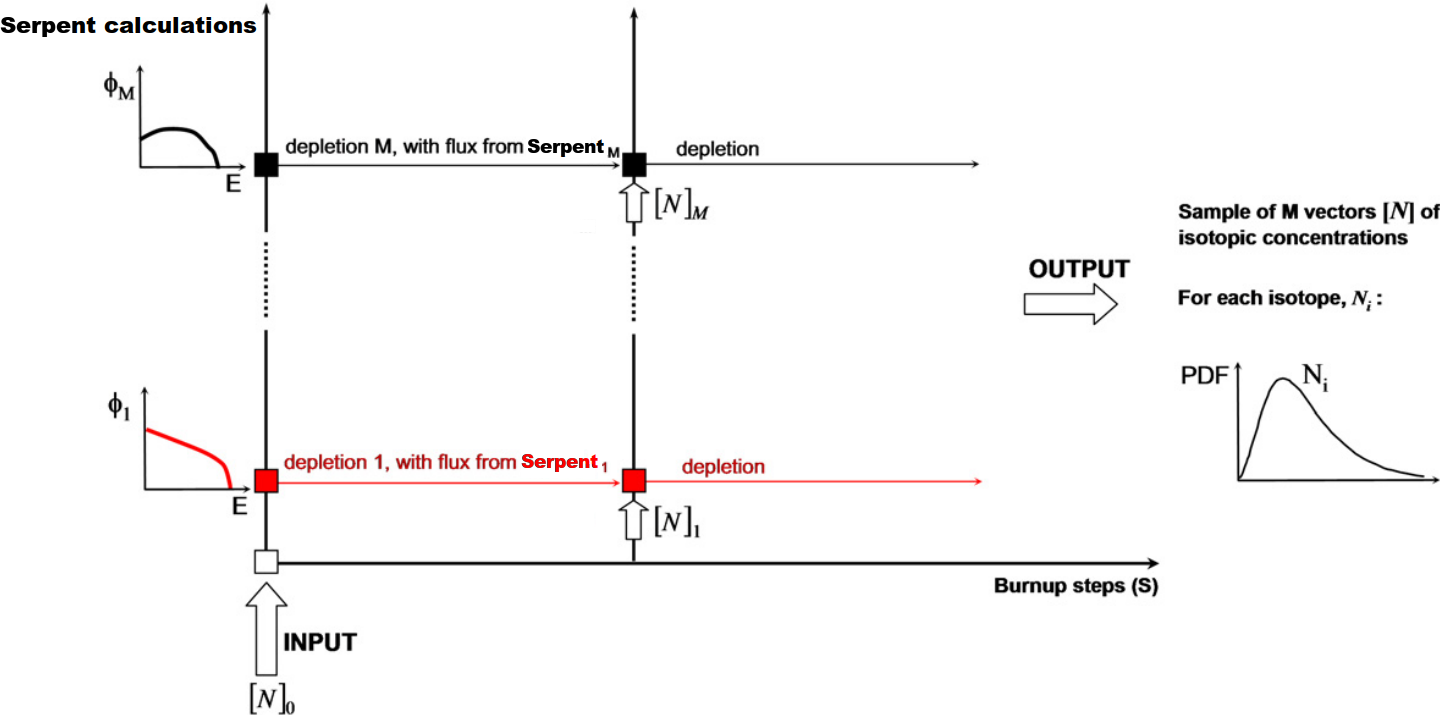
\includegraphics[width=\textwidth]{uq/brute_force_method.png}
	\caption{Methodology of using a normal distribution of random and 
		independent events to estimate uncertainties in final isotopic 
		concentrations (reproduced from Garcia-Herranz \emph{et al.} 
		\cite{garcia-herranz_propagation_2008}). Depletion calculation was 
		performed with the Serpent Monte Carlo code 1000 times by changing only 
		the initial random number.}
	\label{fig:uq-brute-force}
\end{figure}

After running depletion calculations
for all samples, the mean and standard 
deviation of the isotopic concentration can be calculated as
follows
\begin{align}
\overline{N_i} &= \frac{1}{M} \sum_{j=1}^{M} N^{(j)}_i \\
\sigma_{N_i} &= \sqrt{\frac{1}{M-1} \sum_{j=1}^{M} 
	(N^{(j)}_i-\overline{N_j})^2}
\intertext{where}
\overline{N_i} &= \mbox{mean concentration of isotope $i$ $[\frac{1}{cm^3}]$} 
\nonumber \\
M &= \mbox{number of depletion runs with a unique seed $[-]$} 
\nonumber \\
N^{(j)}_i &= \mbox{concentration of isotope $i$ in the sample $j$ 
	$[\frac{1}{cm^3}]$.} 
\nonumber
\end{align}

The isotopic concentration $[N]_j$ can then be propagated throughout the 
criticality calculations to estimate the uncertainty of the multiplication 
factor $k_{eff}$. Serpent Monte Carlo code automatically calculates the mean 
and standard deviation of the $k_{eff}$ in each run $j$, which is 
necessary to find the number of runs (samples) required for the convergence of 
$k_{eff}$.

The \gls{TAP} full-core model in Serpent described earlier (see  
Section~\ref{sec:tap_model}) is used for the uncertainty quantification study 
herein. The model benefits from 1/8 symmetry, which allowed me to 
significantly reduce the computational burden without losing accuracy
(Figure~\ref{fig:tap-serpent-plan}). The number of neutron histories was 
selected to compromise between accuracy and computational costs. Running 
15,000 neutrons with 500 active cycles and 200 inactive cycles 
(used for source convergence) gave a reasonable balance between statistical 
certainty and computation time. Thirty depletion time steps were 
selected for a 30-year depletion simulation (i.e., the isotopic composition is 
stored, and neutron flux is recalculated at the end of each year). 
Additionally, I selected the Chebyshev Rational Approximation Method (CRAM) 
with a predictor-corrector substep \cite{pusa_computing_2010} to reduce 
isotopic 
composition uncertainty. The ENDF/B-VII.1 nuclear data library at 900 K is 
used for all simulations in the current chapter 
\cite{chadwick_endf/b-vii.1_2011}.

\subsection{Results and analysis}
A total of 1000 samples is propagated via the Serpent depletion calculation,  
and the histograms of eigenvalue samples at the \gls{BOL} and \gls{EOL} (30 
\gls{EFPY}) are shown in Figure~\ref{fig:uq-serp-keff-hist}. The 
results show that the mean effective multiplication factor ($k_{eff}$) 
and its standard deviation both decrease gradually during 30 years of 
\gls{TAP} reactor operation due to the stochastic nature of \gls{MC}. 
An uncertainty in $k_{eff}$ of approximately $35$ $pcm$ is observed at the 
\gls{BOL}, while it slipped to about $29$ $pcm$ at the \gls{EOL}. A 1000 
independent Serpent runs were performed on Idaho National Laboratory's Falcon 
supercomputer to obtain a set of M=1000 vectors of isotopic concentrations in 
a depletion simulation with S=30 depletion time intervals each. The 
computational time for such an analysis was approximately 1,200 node-hours 
(4.9 core-years).
\begin{figure}[htp!] % replace 't' with 'b' to 
	\centering
	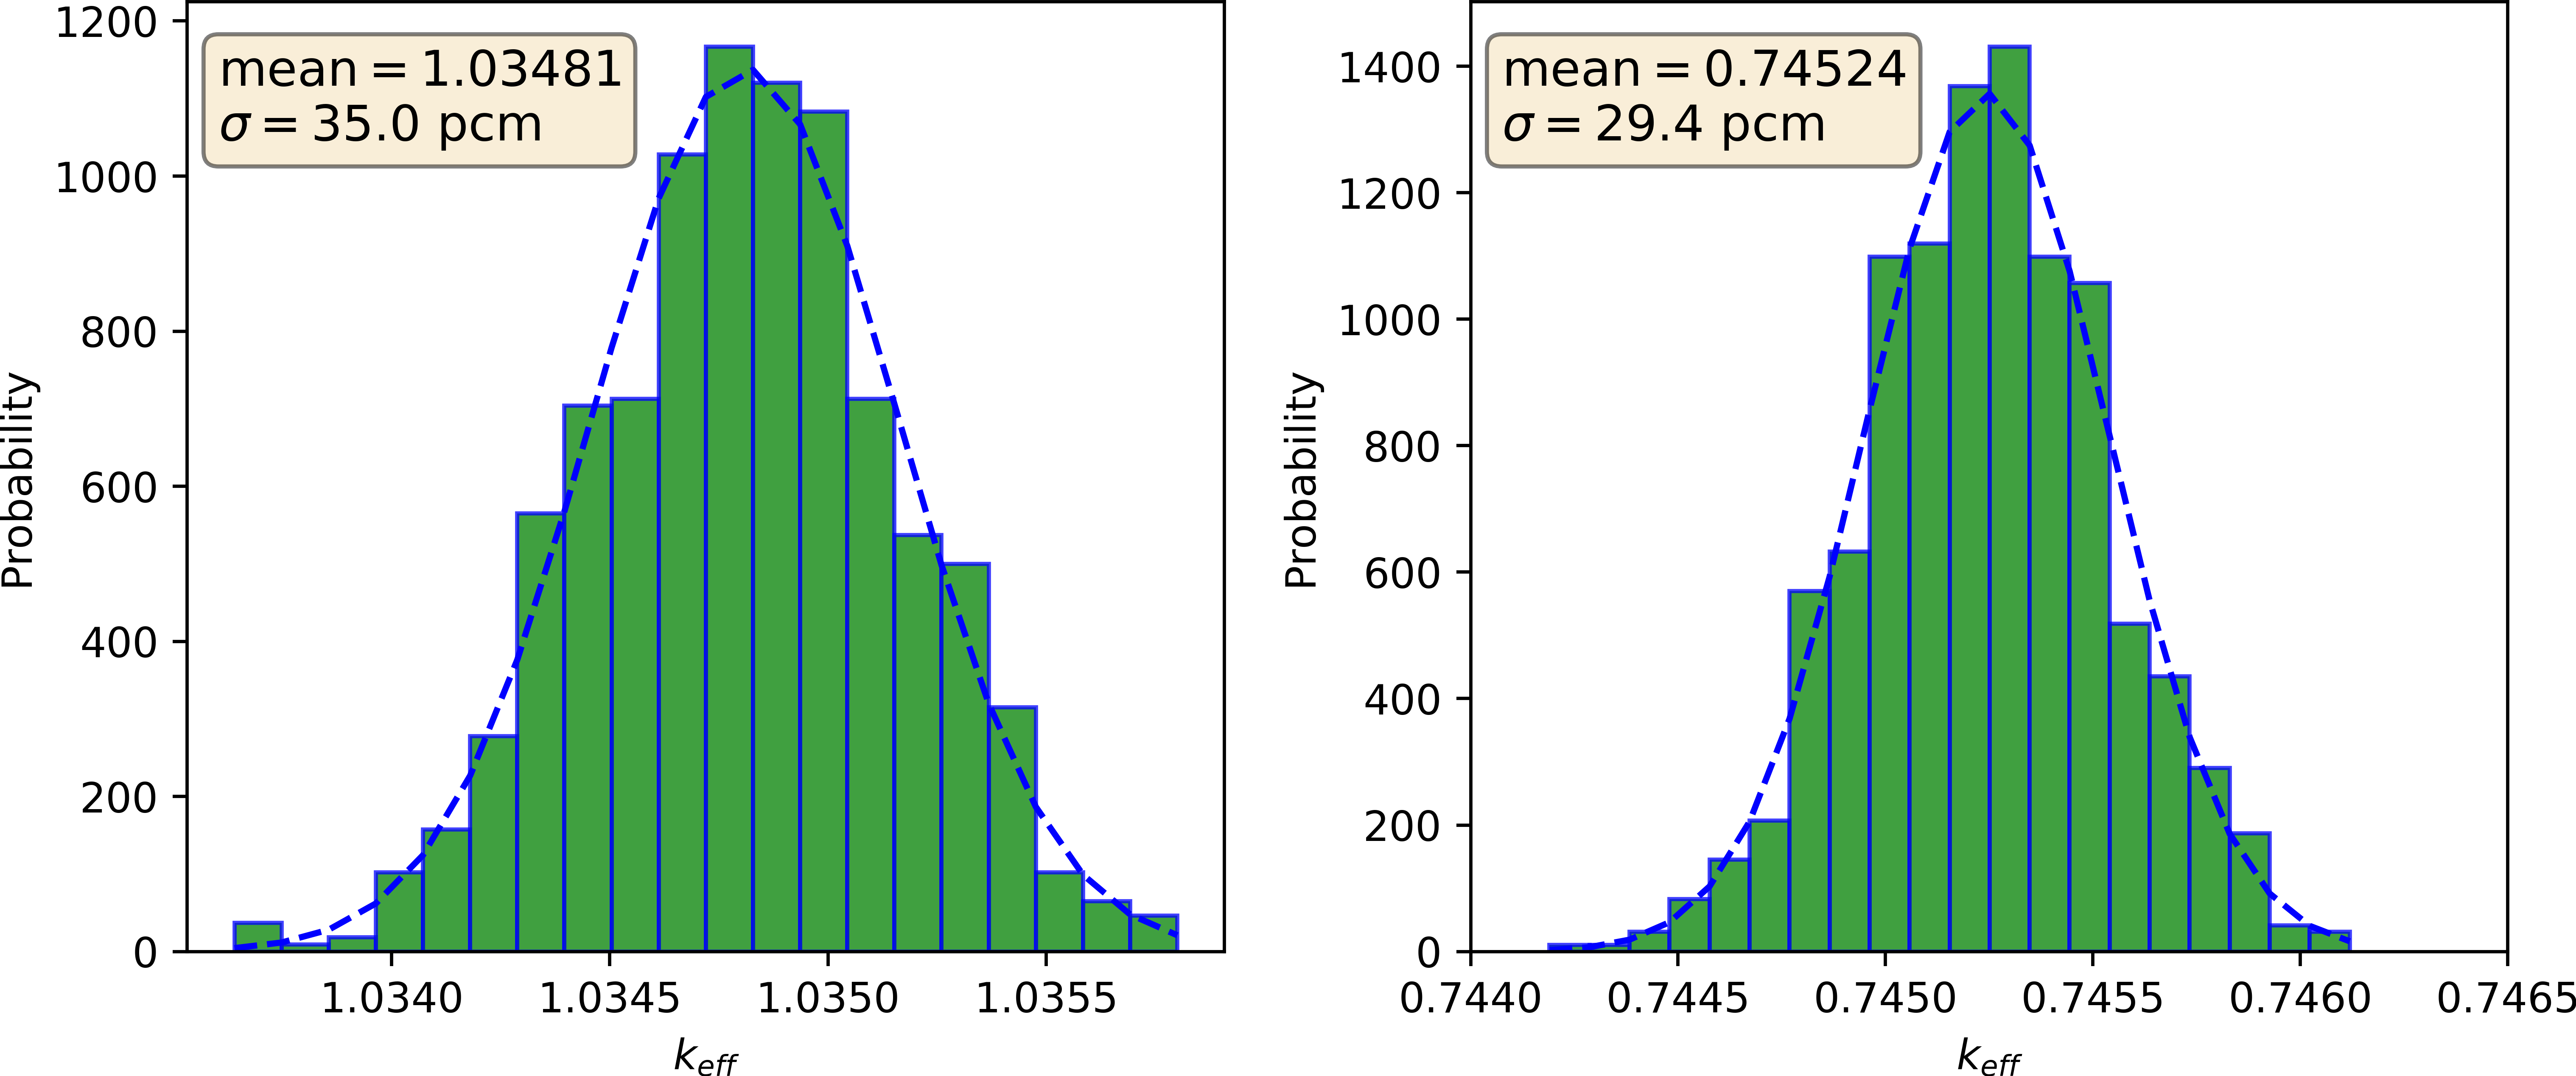
\includegraphics[width=\textwidth]{uq/endf_serpent_keff_hist_for_tap.png}
	\vspace{-4mm}
	\caption{Histograms of $k_{eff}$ samples obtained with 1000 independent 
		Serpent depletion calculations at the \gls{BOL} (left) and \gls{EOL} 
		(right).}
	\label{fig:uq-serp-keff-hist}
\end{figure}

Figure~\ref{fig:uq-serpent-keff-evolution} shows the observed and reported by 
Serpent uncertainties in $k_{eff}$ for the \gls{TAP} core during 30 years of 
operation. Notably, Serpent-calculated uncertainty in the multiplication 
factor is slightly lower than observed uncertainty. This discrepancy is due to 
statistical noise in the pseudo-randomly generated initial seed and agreed 
with results in the literature 
\cite{wyant_numerical_2012}. Across all 30 depletion steps, the mean observed 
and reported uncertainty in the $k_{eff}$ is $30$ and $25$ $pcm$, 
respectively. A better match in these values could be obtained with more 
samples $M$ (e.g., $M=10,\!000$), which would require substantially more 
computational power.
\begin{figure}[hbp!] % replace 't' with 'b' to 
	\centering
	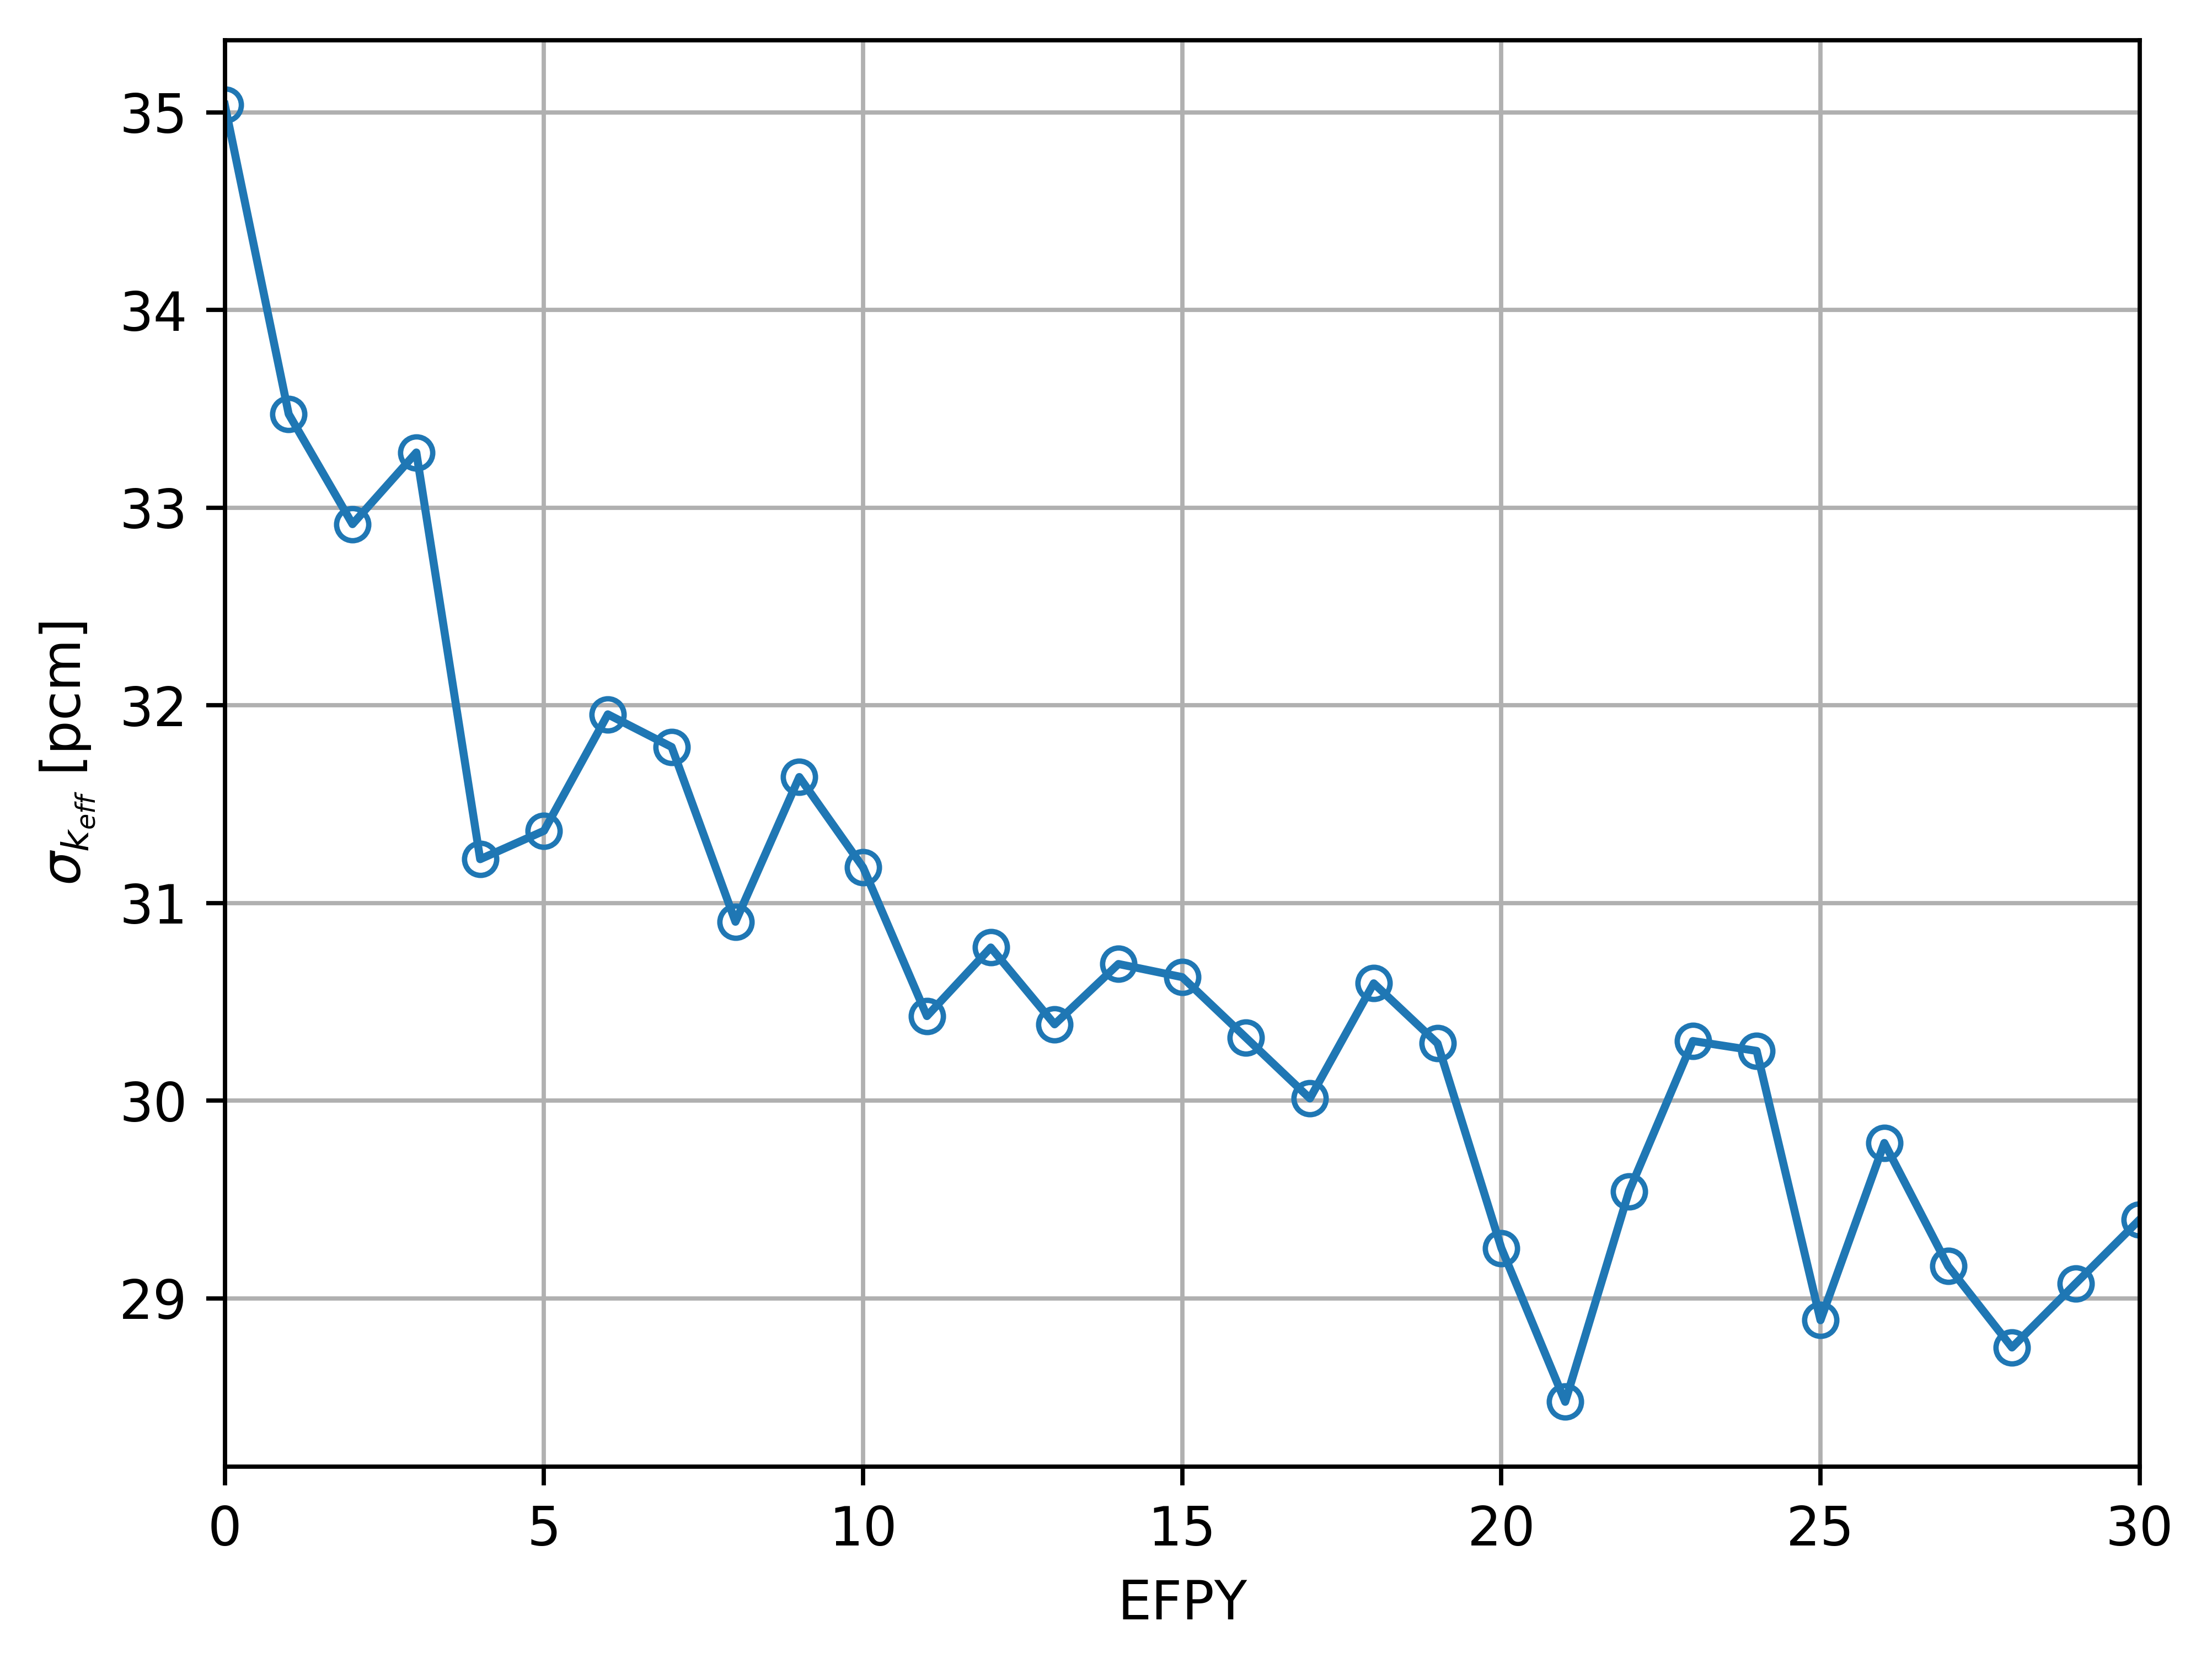
\includegraphics[width=0.83\textwidth]{uq/endf_serpent_keff_dynamics_for_tap.png}
	\caption{Observed and reported by Serpent uncertainty of the effective 
		multiplication factor ($\sigma_{k_{eff}}$) for the full-core \gls{TAP} 
		core model during 30 years of operation.}
	\label{fig:uq-serpent-keff-evolution}
\end{figure}

The current depletion algorithm in Serpent uses the neutron flux solution 
obtained from the \gls{MC} neutron histories to solve the Bateman equations to 
find the isotopic inventory evolution. As was discussed earlier, Serpent 
is unable to estimate the uncertainty of the isotopic number density like it 
does for the $k_{eff}$ (reported $\sigma_{k_{eff}}$ in 
Figure~\ref{fig:uq-serpent-keff-evolution}). Thus, to gain insight into the 
uncertainties in the isotopic inventory, the standard deviation in observed 
isotopic inventories from the 1000 depletion runs was investigated. The 
observed uncertainties for the major actinides and poisonous \glspl{FP} 
resulting from depletion calculations are shown on  
Figures~\ref{fig:uq-serpent-u}, \ref{fig:uq-serpent-pu}, and 
\ref{fig:uq-serpent-xe-i}.

\begin{figure}[htp!] % replace 't' with 'b' to 
	\centering
	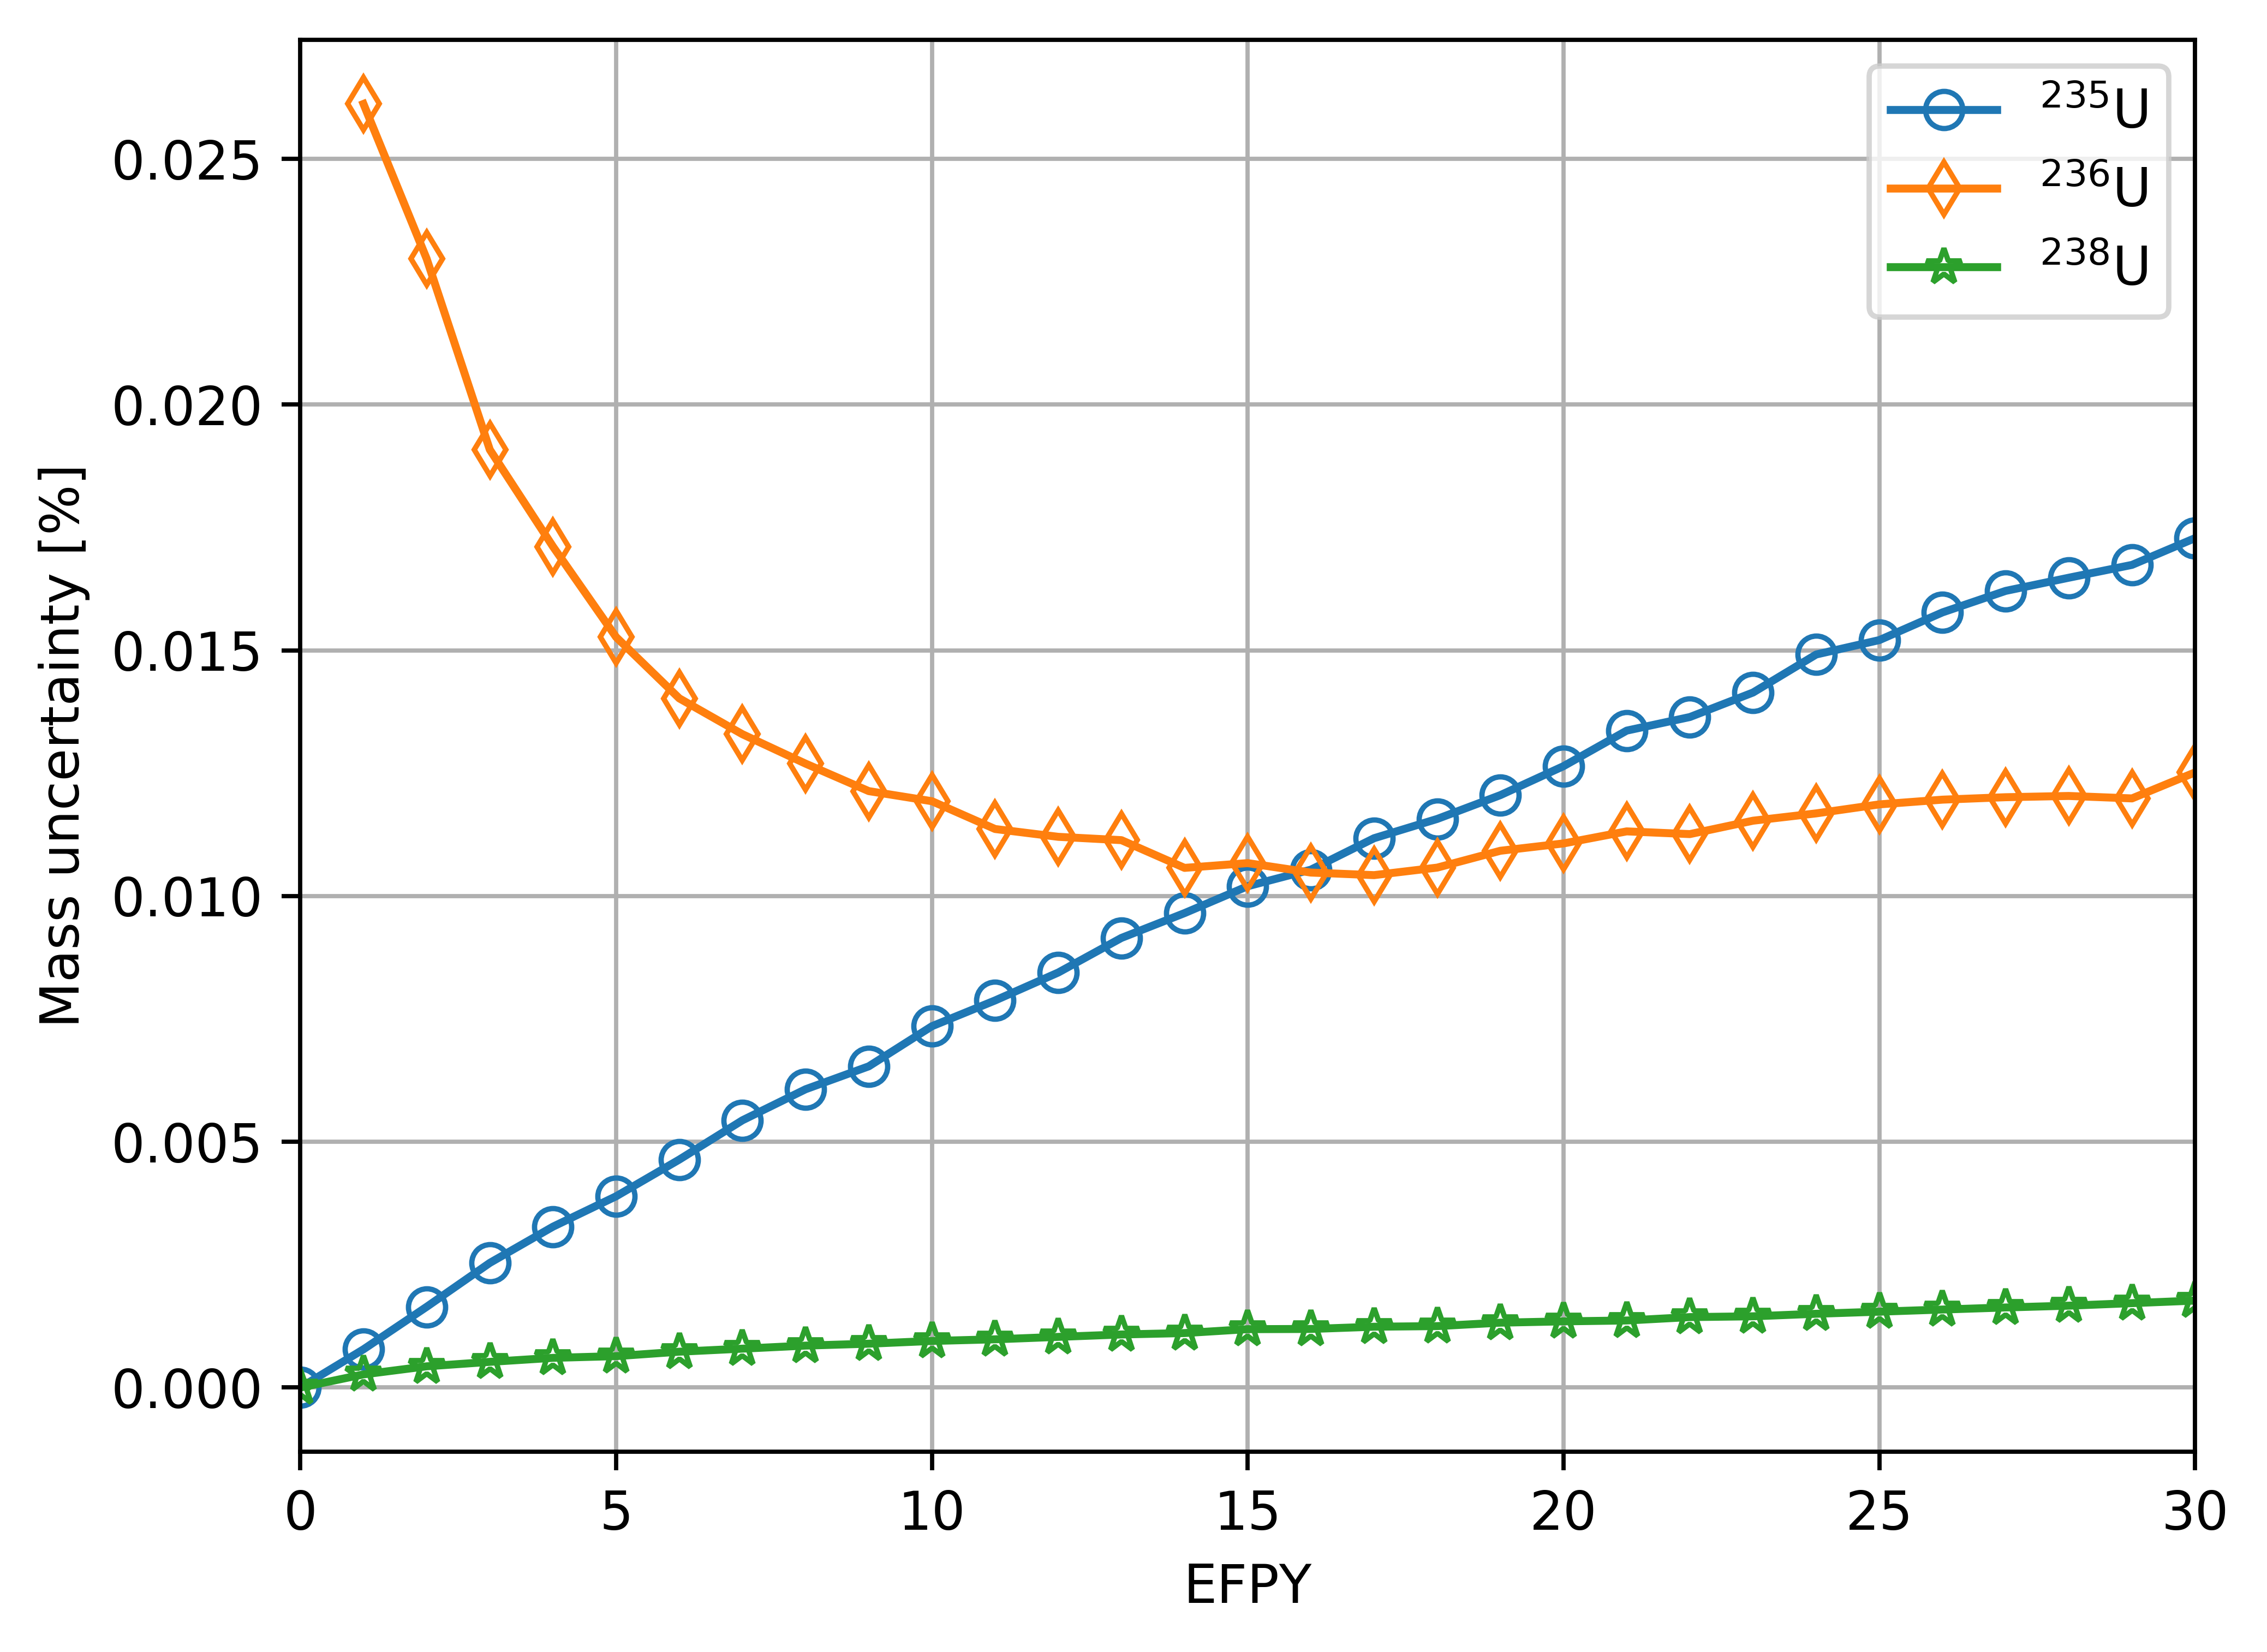
\includegraphics[width=0.8\textwidth]{uq/serpent_mass_std_u.png}
	\vspace{-4mm}
	\caption{Stochastic uncertainty evolution in the uranium isotopic 
		inventory during 30 years of depletion.}
	\label{fig:uq-serpent-u}
\end{figure}

The relative uncertainty of $^{235}$U mass increases with time due to its 
depletion, as the uranium enrichment steadily decreases from 5\% to 0.7\%.
The uncertainty of $^{236}$U mass is 
0.026\% after 30 days of operation when only a few grams of this isotope were 
produced in the core. The uncertainty of $^{236}$U is between 0.011\% and 
0.013\% once the $^{236}$U approaches its equilibrium concentration. The 
relative uncertainties of fissile $^{239}$Pu and $^{241}$Pu are 0.01-0.07\% 
and 0.04-0.18\%, respectively. Mass uncertainties for the 
strongest neutron poison, $^{135}$Xe, and its primary direct precursor, 
$^{135}$I, are 0.0175-0.0275\% and 0.01-0.0175\%, respectively. Overall, 
stochastic error in depletion calculations is larger for isotopes with small 
concentrations in the core due to round-off error. 
Table~\ref{tab:uq-serpent-mean-std-rsd} shows that the stochastic error in the 
isotopic inventories even for an unusually high burnup of 100 MW$_{th}$d/kgU 
(30 EFPY) is negligible ($<0.1$\%).

\begin{figure}[htp!] % replace 't' with 'b' to 
	\centering
	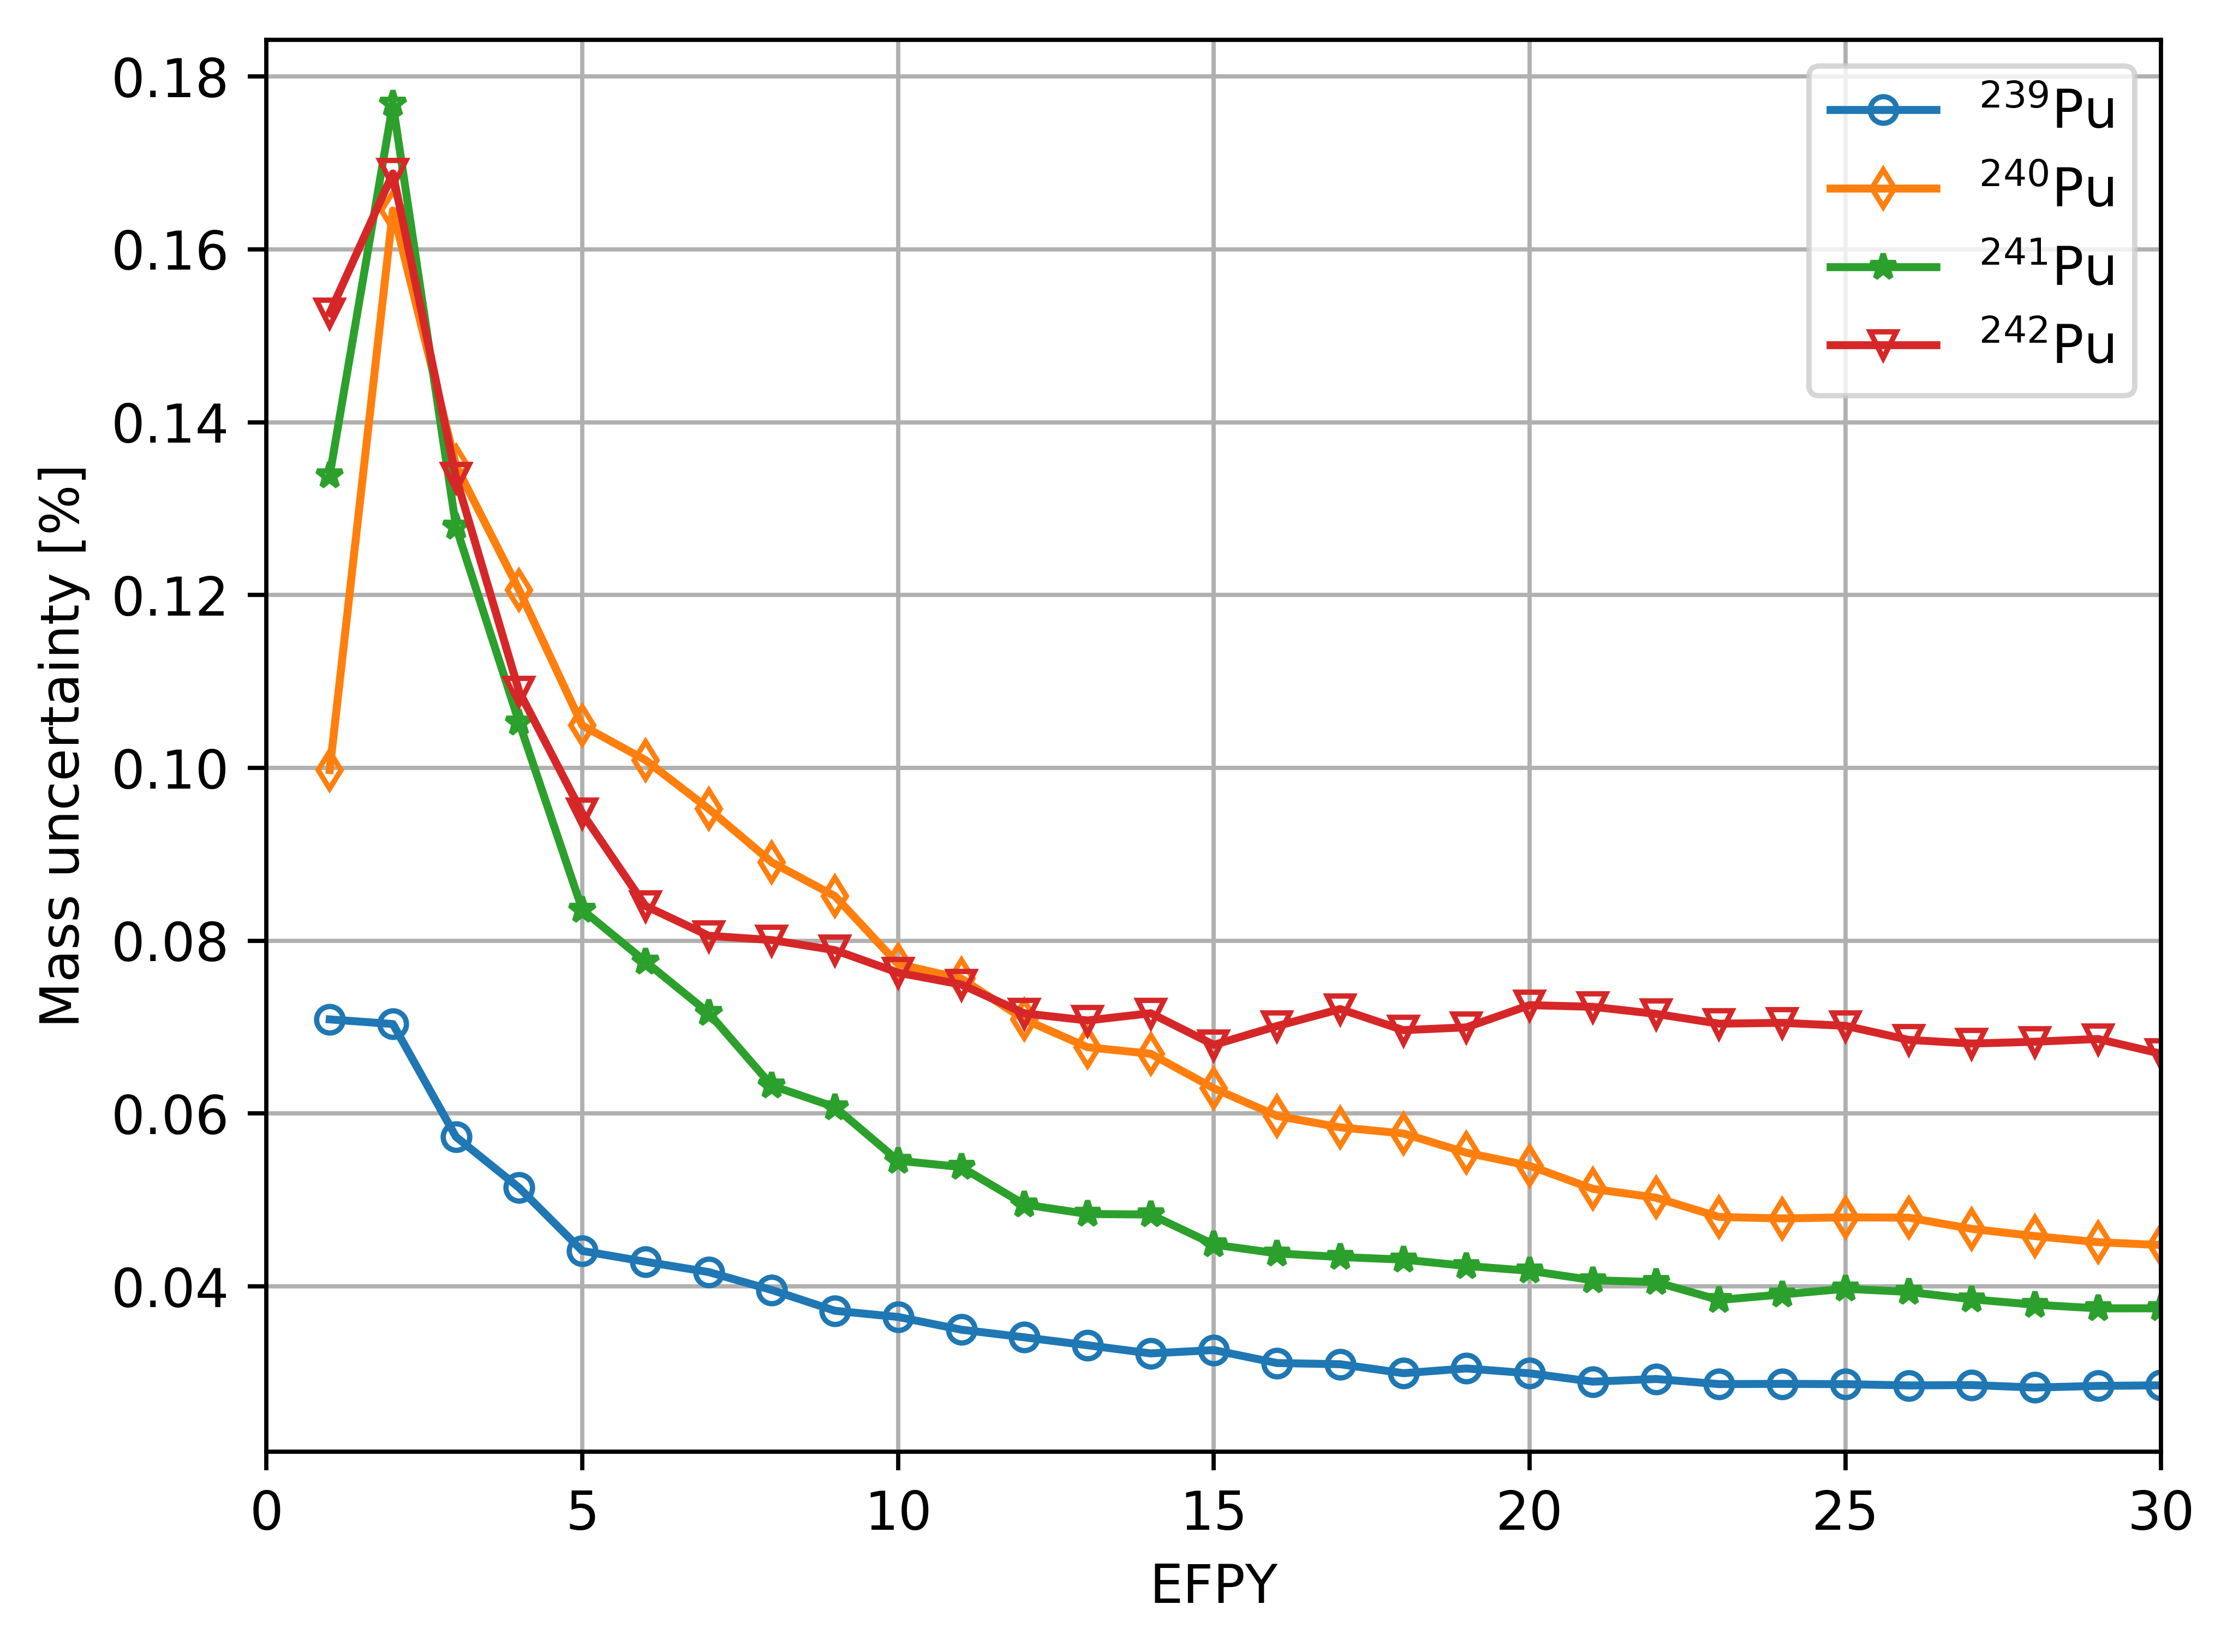
\includegraphics[width=0.73\textwidth]{uq/serpent_mass_std_pu.png}
	\vspace{-3mm}
	\caption{Stochastic uncertainty evolution in the plutonium isotopic 
		inventory during 30 years of depletion.}
	\label{fig:uq-serpent-pu}
\end{figure}
\vspace{-9mm}
\begin{figure}[hbp!] % replace 't' with 'b' to 
	\centering
	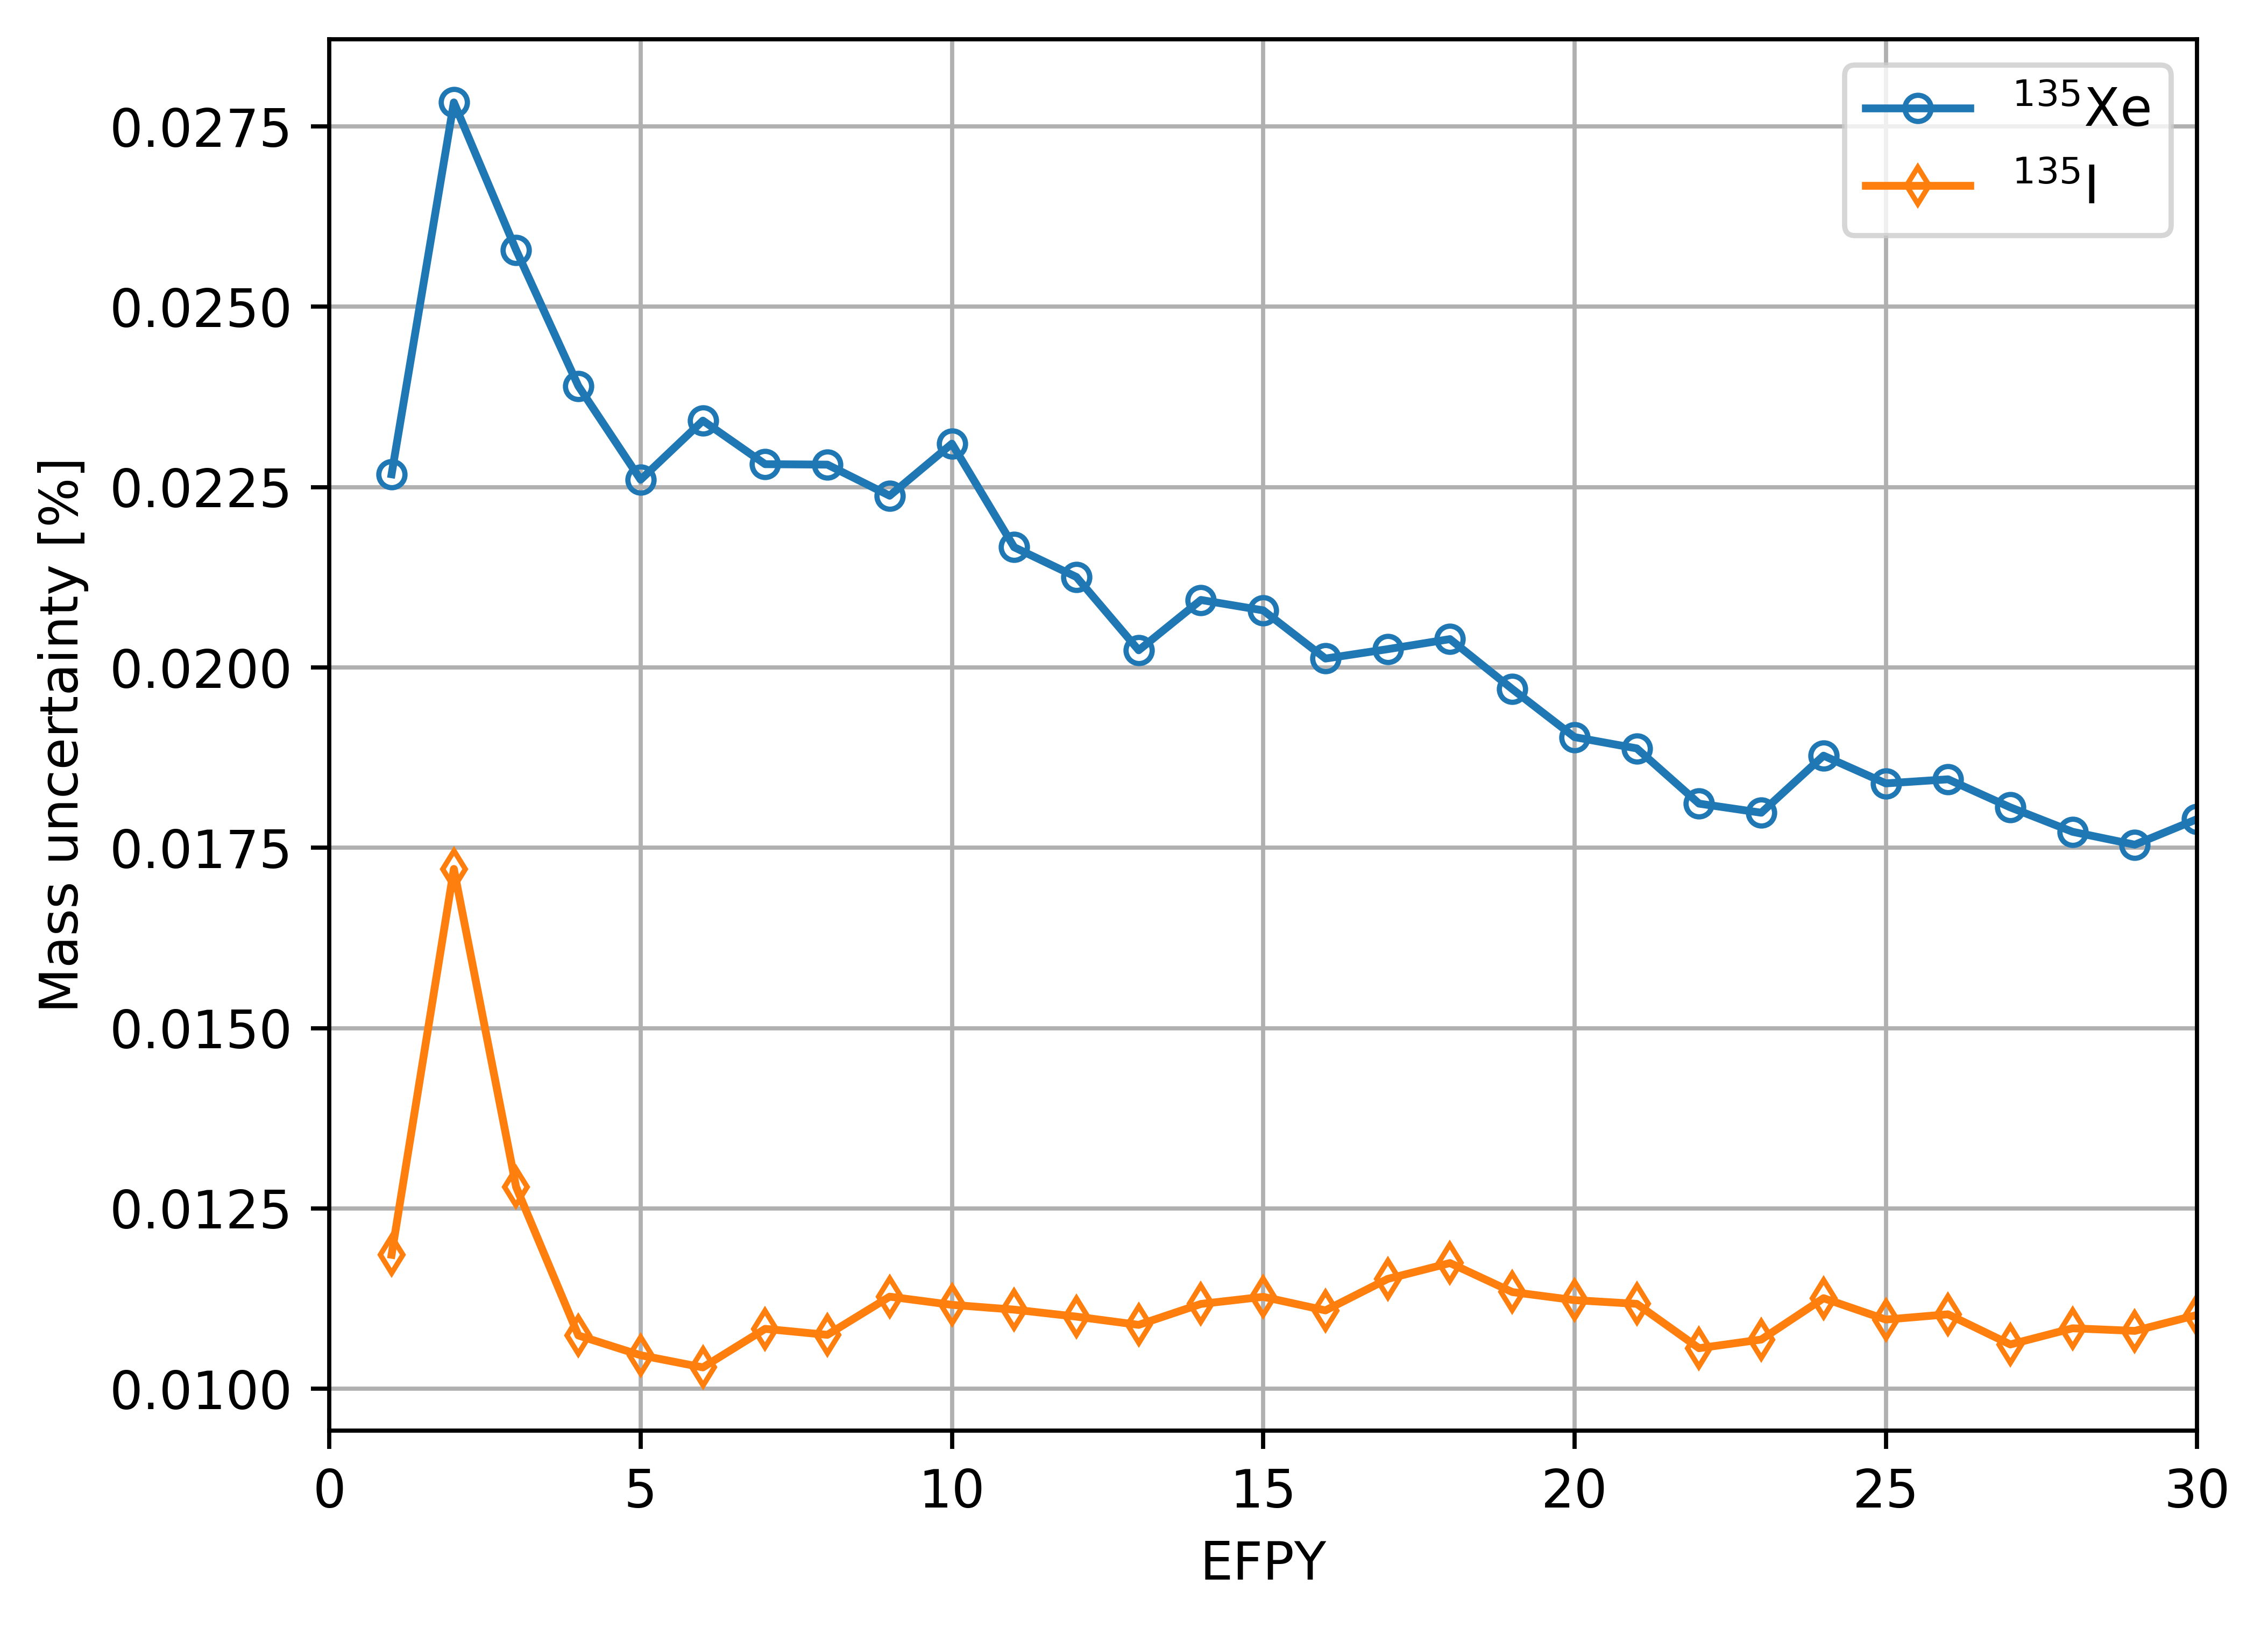
\includegraphics[width=0.73\textwidth]{uq/serpent_mass_std_xe_i.png}
	\vspace{-3mm}
	\caption{Stochastic uncertainty evolution in $^{135}$Xe and $^{135}$I 
		isotopic inventory during 30 years of depletion.}
	\label{fig:uq-serpent-xe-i}
\end{figure}


%%%%%%%%%%%%%%%%%%%%%%%%%%%%%%%%%%%%%%%%
\begin{table}[htp!]
	\centering
	\caption{Mean value, Standard Deviation (STD), and Relative Standard 
		Deviation (RSD) of mass for the major isotopes after 30-year depletion 
		analysis for the \gls{TAP} reactor. Only the stochastic error in the 
		Monte 
		Carlo calculations is considered.}
	\begin{tabularx}{0.7\textwidth}{L R R R R}
		\hline
		\textbf{Isotope}  & \textbf{Mean ($\mu$) [kg]} & \textbf{STD 
			($\sigma$) [kg]} & \textbf{RSD ($\sigma/\mu$) [\%]}\\ \hline
		$^{234}$U  & 25.8  & 0.0075 & 0.0290\% \\
		$^{235}$U  & 789.9 & 0.1365 & 0.0173\% \\
		$^{236}$U  & 1149.5& 0.1439 & 0.0125\% \\
		$^{238}$U  & 112,084.8 & 1.9835 & 0.0018\% \\
		$^{238}$Pu & 405.5 & 0.0884 & 0.0218\% \\
		$^{239}$Pu & 5554.3& 1.5860 & 0.0286\% \\
		$^{240}$Pu & 1230.2& 0.5510 & 0.0448\% \\
		$^{241}$Pu & 763.1 & 0.2859 & 0.0375\% \\
		$^{242}$Pu & 139.0 & 0.0930  & 0.0669\% \\
		$^{241}$Am & 218.3 & 0.0566  & 0.0259\% \\
		$^{135}$Xe & 0.03  & $<0.0001$& 0.0179\% \\
		$^{135}$I  & 0.02  & $<0.0001$& 0.0110\% \\ \hline
	\end{tabularx}
	\label{tab:uq-serpent-mean-std-rsd}
	\vspace{-0.9em}
\end{table}
%%%%%%%%%%%%%%%%%%%%%%%%%%%%%%%%%%%%%%%%%%%%%%%%%%%%%%%%%%%%%%%%%%%%%%%%%%%%%%%

All results presented in Figures~\ref{fig:uq-serpent-u},  
\ref{fig:uq-serpent-pu}, \ref{fig:uq-serpent-xe-i}, and  
Table~\ref{tab:uq-serpent-mean-std-rsd} are based on 1000 samples (e.g., 1000 
independent Serpent depletion simulations with unique random seeds). 
Figure~\ref{fig:uq-serpent-convergence} shows the 
convergence of $k_{eff}$ and $^{235}$U mass uncertainty with the number of 
samples. Notably, 300 samples were enough for $\sigma_{k_{eff}}$ convergence. 
The $^{235}$U mass uncertainty at the \gls{EOL} decreases steadily 
with the number of samples, but even 400 samples are sufficient to obtain 
reasonable uncertainty ($<0.02$\%). 
Finally, it is possible to reduce the stochastic uncertainty in the isotopic 
inventory to almost zero by substantially increasing the neutron population 
(number of neutron histories and active cycles). However, this is extremely 
inefficient because Monte Carlo converges sublinearly ($O(\sqrt{N})$).
\begin{figure}[htp!] % replace 't' with 'b' to 
	\centering
	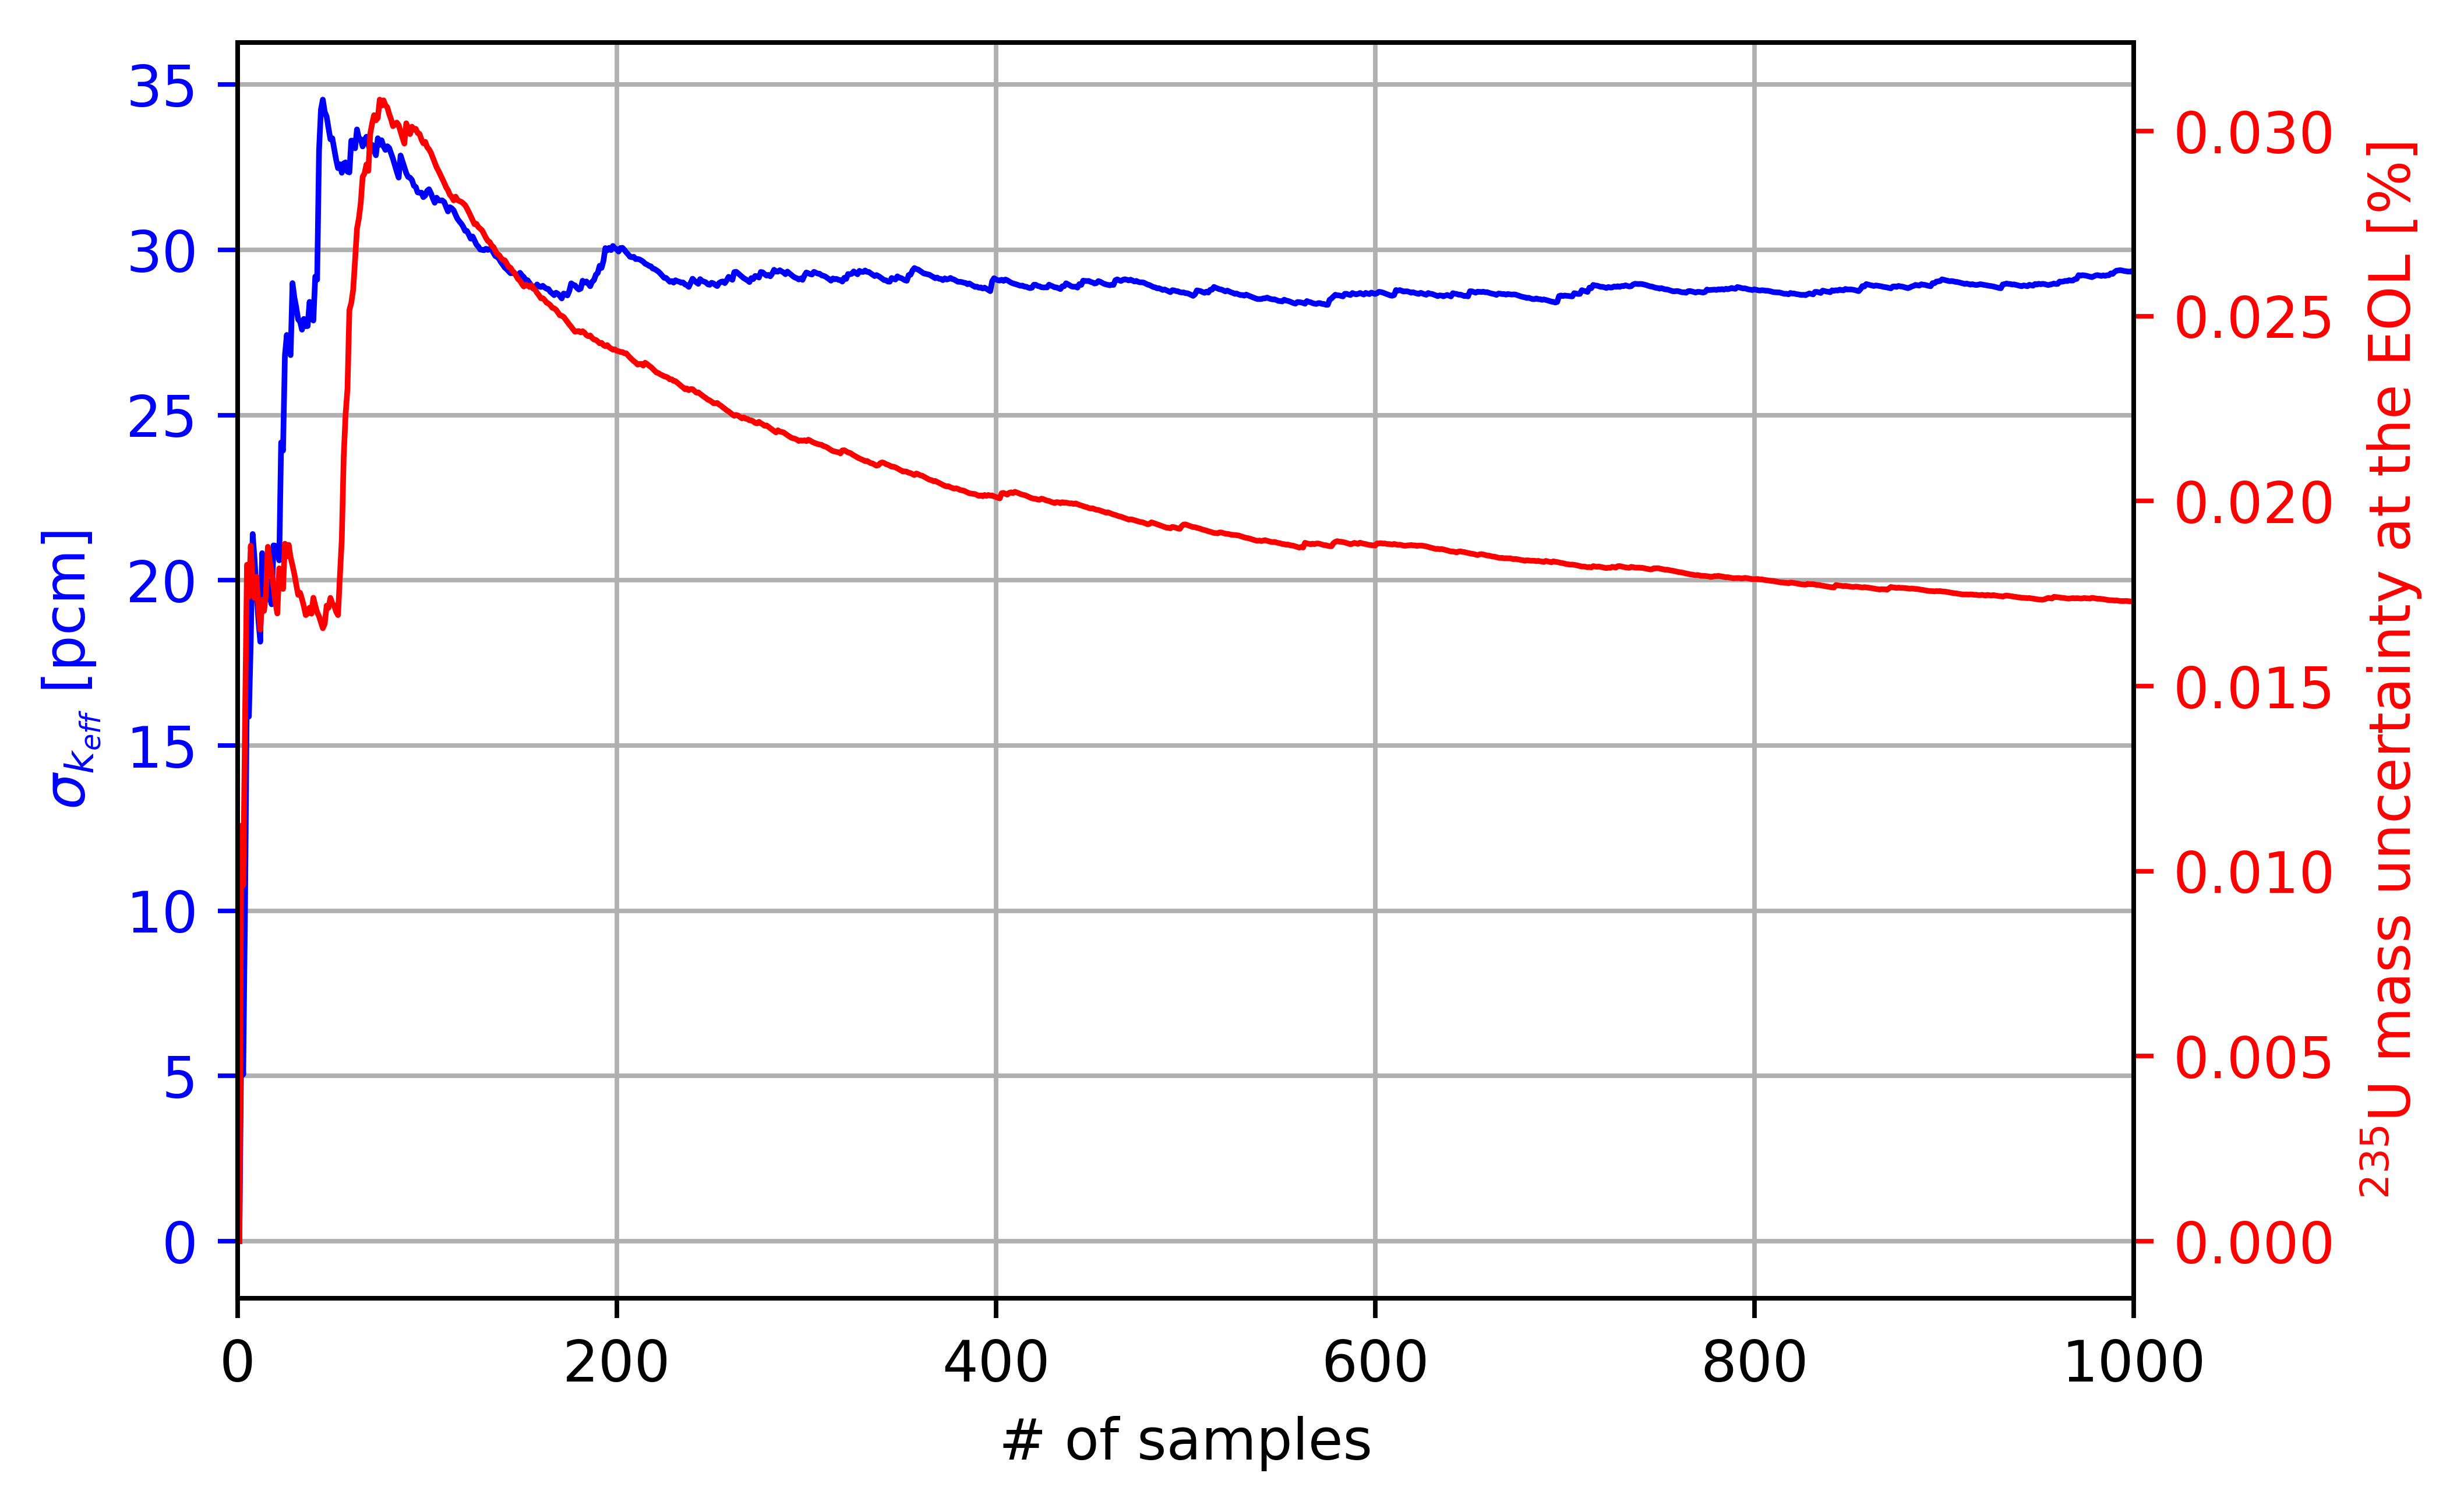
\includegraphics[width=\textwidth]{uq/serpent_convergance_for_tap.png}
	\caption{Convergence of $k_{eff}$ and $^{235}$U mass uncertainties due to 
		the statistical error in Monte Carlo as a function of number of 
		samples.}
	\label{fig:uq-serpent-convergence}
\end{figure}
\FloatBarrier


\section{Nuclear data-related uncertainty in the isotopic inventory}
This section focuses on evaluating uncertainty in a depletion calculation 
caused by uncertainties in nuclear data, namely, cross sections, fission 
yields, and decay constants. I used a deterministic $S_N$ transport solver, 
SCALE/TRITON \cite{rearden_scale_2018}, to avoid statistical errors and 
isolate nuclear data-related uncertainty.

\subsection{Methodology of uncertainty propagation by a random sampling}
Nuclear data uncertainties are propagated through fuel depletion calculations 
using a random sampling method\footnote{Sometimes researchers also 
	called it ``Monte Carlo sampling," \cite{radaideh_using_2019} ``brute 
	force method,"\cite{garcia-herranz_propagation_2008} or ``Fast Total Monte 
	Carlo" \cite{rochman_nuclear_2014}. However, in this chapter, this method 
	is 
	called ``random  sampling."}. The multi-step sequence of deterministic 
neutronics and isotopic transmutation could be regarded as a single 
process with input parameters (cross sections, fission yields, decay 
constants) and an output (isotopic inventory). This sequence runs a 
large number of times, each time using a different nuclear data file (sample). 
This collection of random nuclear data files is produced by the SCALE Sampler 
module from a multivariate normal distribution using covariance matrices in 
the 56-group covariance library \cite{rearden_scale_2018, 
	radaideh_novel_2019}. This approach is summarized in the flowchart 
(Figure~\ref{fig:uq-sampler}).

After generating the collection of random nuclear data files, SCALE performs 
depletion calculations for each sample. This work uses NEWT, a
2D-deterministic transport code, coupled with ORIGEN. ORIGEN solves a set of 
the Bateman equations using NEWT-calculated neutron fluxes. The unit cell 
model is used to achieve reasonable computing costs while providing an 
accurate neutron spectrum for depletion calculations 
(Figure~\ref{fig:uq-tap-pincell}) \cite{betzler_molten_2017, 
	rykhlevskii_fuel_2019, betzler_modeling_2020}. For this unit cell model, an 
8$\times$8 mesh with reflective boundary conditions is used. The 56-group 
ENDF/B-VII.1 nuclear data library along with the 56-group covariance library 
are used in these depletion calculations. 
%The full-core 3-D depletion 
%calculation can be performed if NEWT is replaced with KENO-VI, which 
%is a three-dimensional Monte Carlo neutron transport code, that might be 
%coupled with ORIGEN for performing depletion calculations. However, two 
%reasons make it impractical because: 
%(1) it requires enormous computing cost, (2) it introduces stochastic error 
%due to the statistical nature of the \gls{MC} method, and 
%(3) it cannot be applied to continuous energy Monte Carlo calculations 
%\cite{rearden_scale_2018}.
\begin{figure}[htp!] % replace 't' with 'b' to 
	\centering
	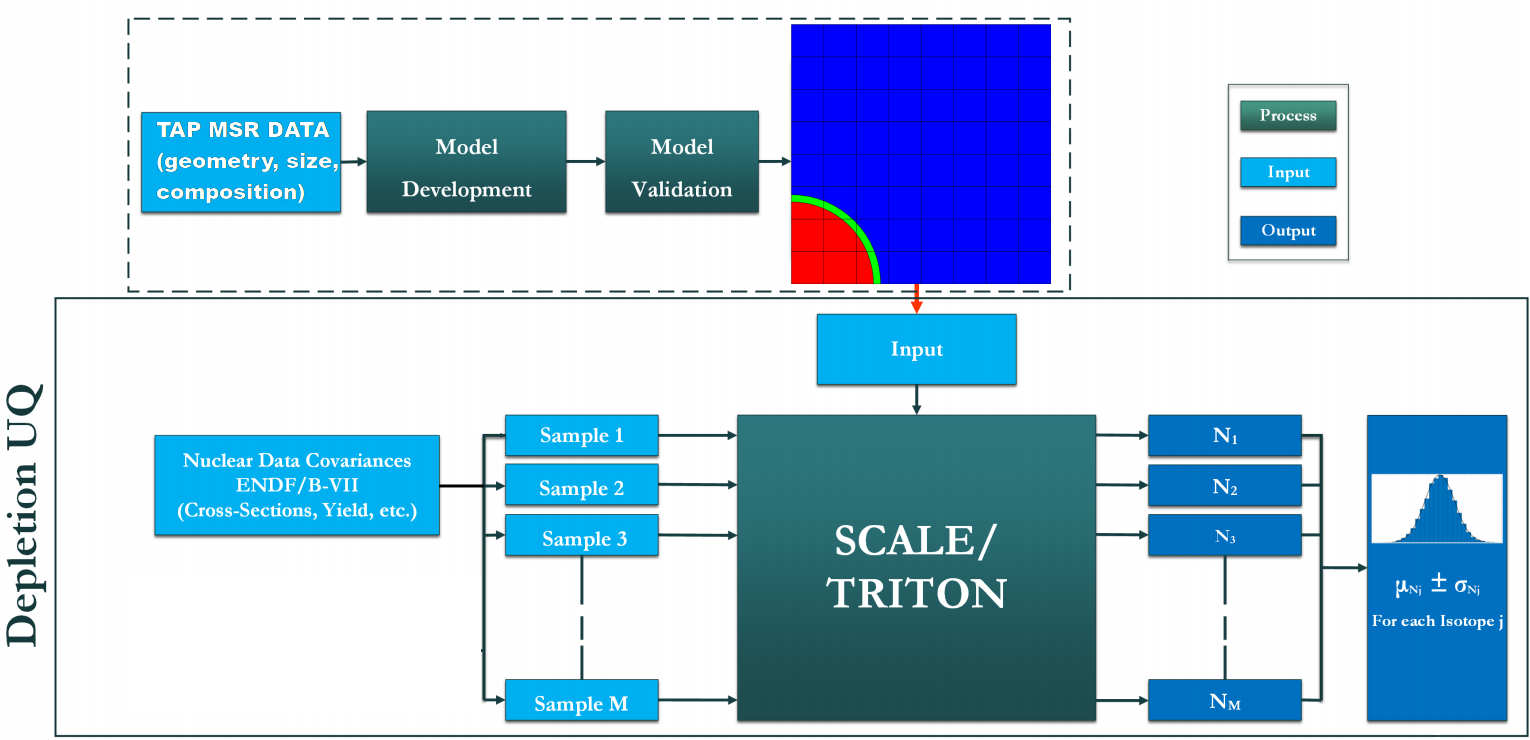
\includegraphics[width=\textwidth]{uq/majdi_scale_scheme.png}
	\caption{Flowchart of depletion uncertainty quantification 
		using SCALE Sampler (figure courtesy of Majdi I. Radaideh 
		\cite{radaideh_novel_2019}).}
	\label{fig:uq-sampler}
\end{figure}
\vspace{-7mm}
\begin{figure}[hbp!] % replace 't' with 'b' to 
	\centering
	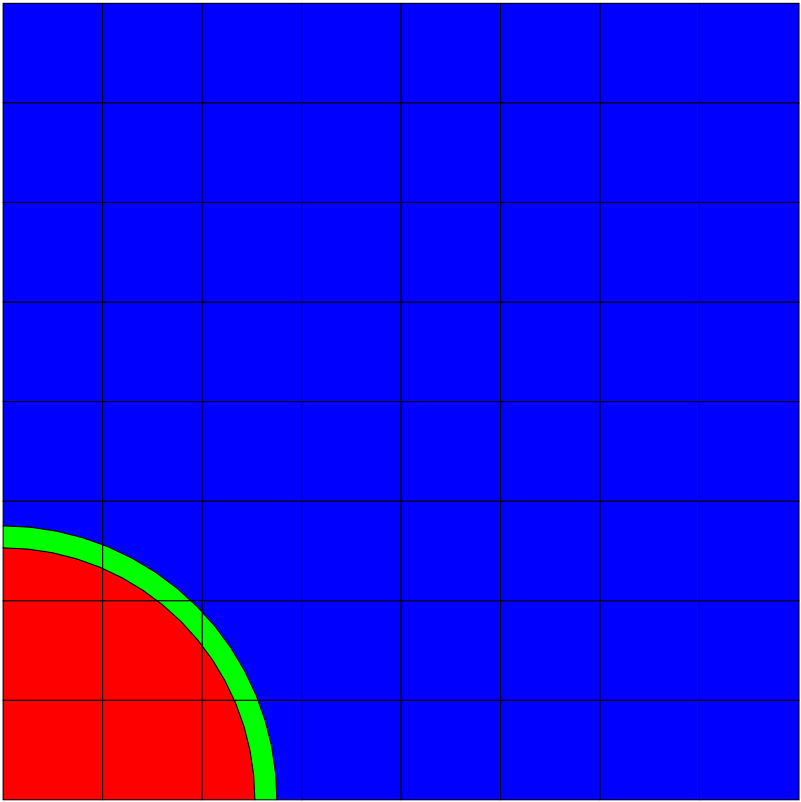
\includegraphics[width=0.41\textwidth]{uq/tap_pin_for_scale.png}
	\caption{Unit cell model representation for the \gls{TAP} \gls{MSR} in 
		SCALE.}
	\label{fig:uq-tap-pincell}
\end{figure}

The fuel salt composition, total depletion time, depletion time steps, and 
power density match the ones given in Section~\ref{sec:uq-stochastic} for 
consistency of comparison. Overall, I repeated 800 SCALE depletion 
calculations using perturbed cross sections, fission yields, and decay 
constants, assuming that the probability density functions are multivariate 
normal distributions with covariances provided with the SCALE nuclear data 
library.


\subsection{Results and analysis}
Figure~\ref{fig:uq-scale-kinf-hist} shows histograms of the 
infinite multiplication factor ($k_{\infty}$) at the \gls{BOL} and \gls{EOL} 
(30 \gls{EFPY}) for 800 total random samples. Similar to stochastic 
uncertainty, the results show that the $k_{\infty}$ standard deviation due to 
the nuclear data uncertainty decreases during 30 years of the \gls{TAP} 
reactor operation. An uncertainty of about 804 $pcm$ in $k_{\infty}$ is 
observed at startup, while it is reduced to 469 $pcm$ at the \gls{EOL}. 
Notably, nuclear data-related uncertainty in the multiplication factor is 
about 20 times larger than uncertainty due to the stochastic error (see 
Section~\ref{sec:uq-stochastic}), which agrees well with results in the 
literature \cite{takeda_estimation_1999, garcia-herranz_propagation_2008}. 
Thanks to the unit cell model and a fast deterministic $S_N$ NEWT transport 
code, the computational time for producing 800 random samples was only 576 
core-days. Generation of the 800 samples with better accuracy (full-core, 
three-dimensional model solved with KENO-VI) would require substantially more 
computational power (about 10,000 times more).
\begin{figure}[htp!] % replace 't' with 'b' to 
	\centering
	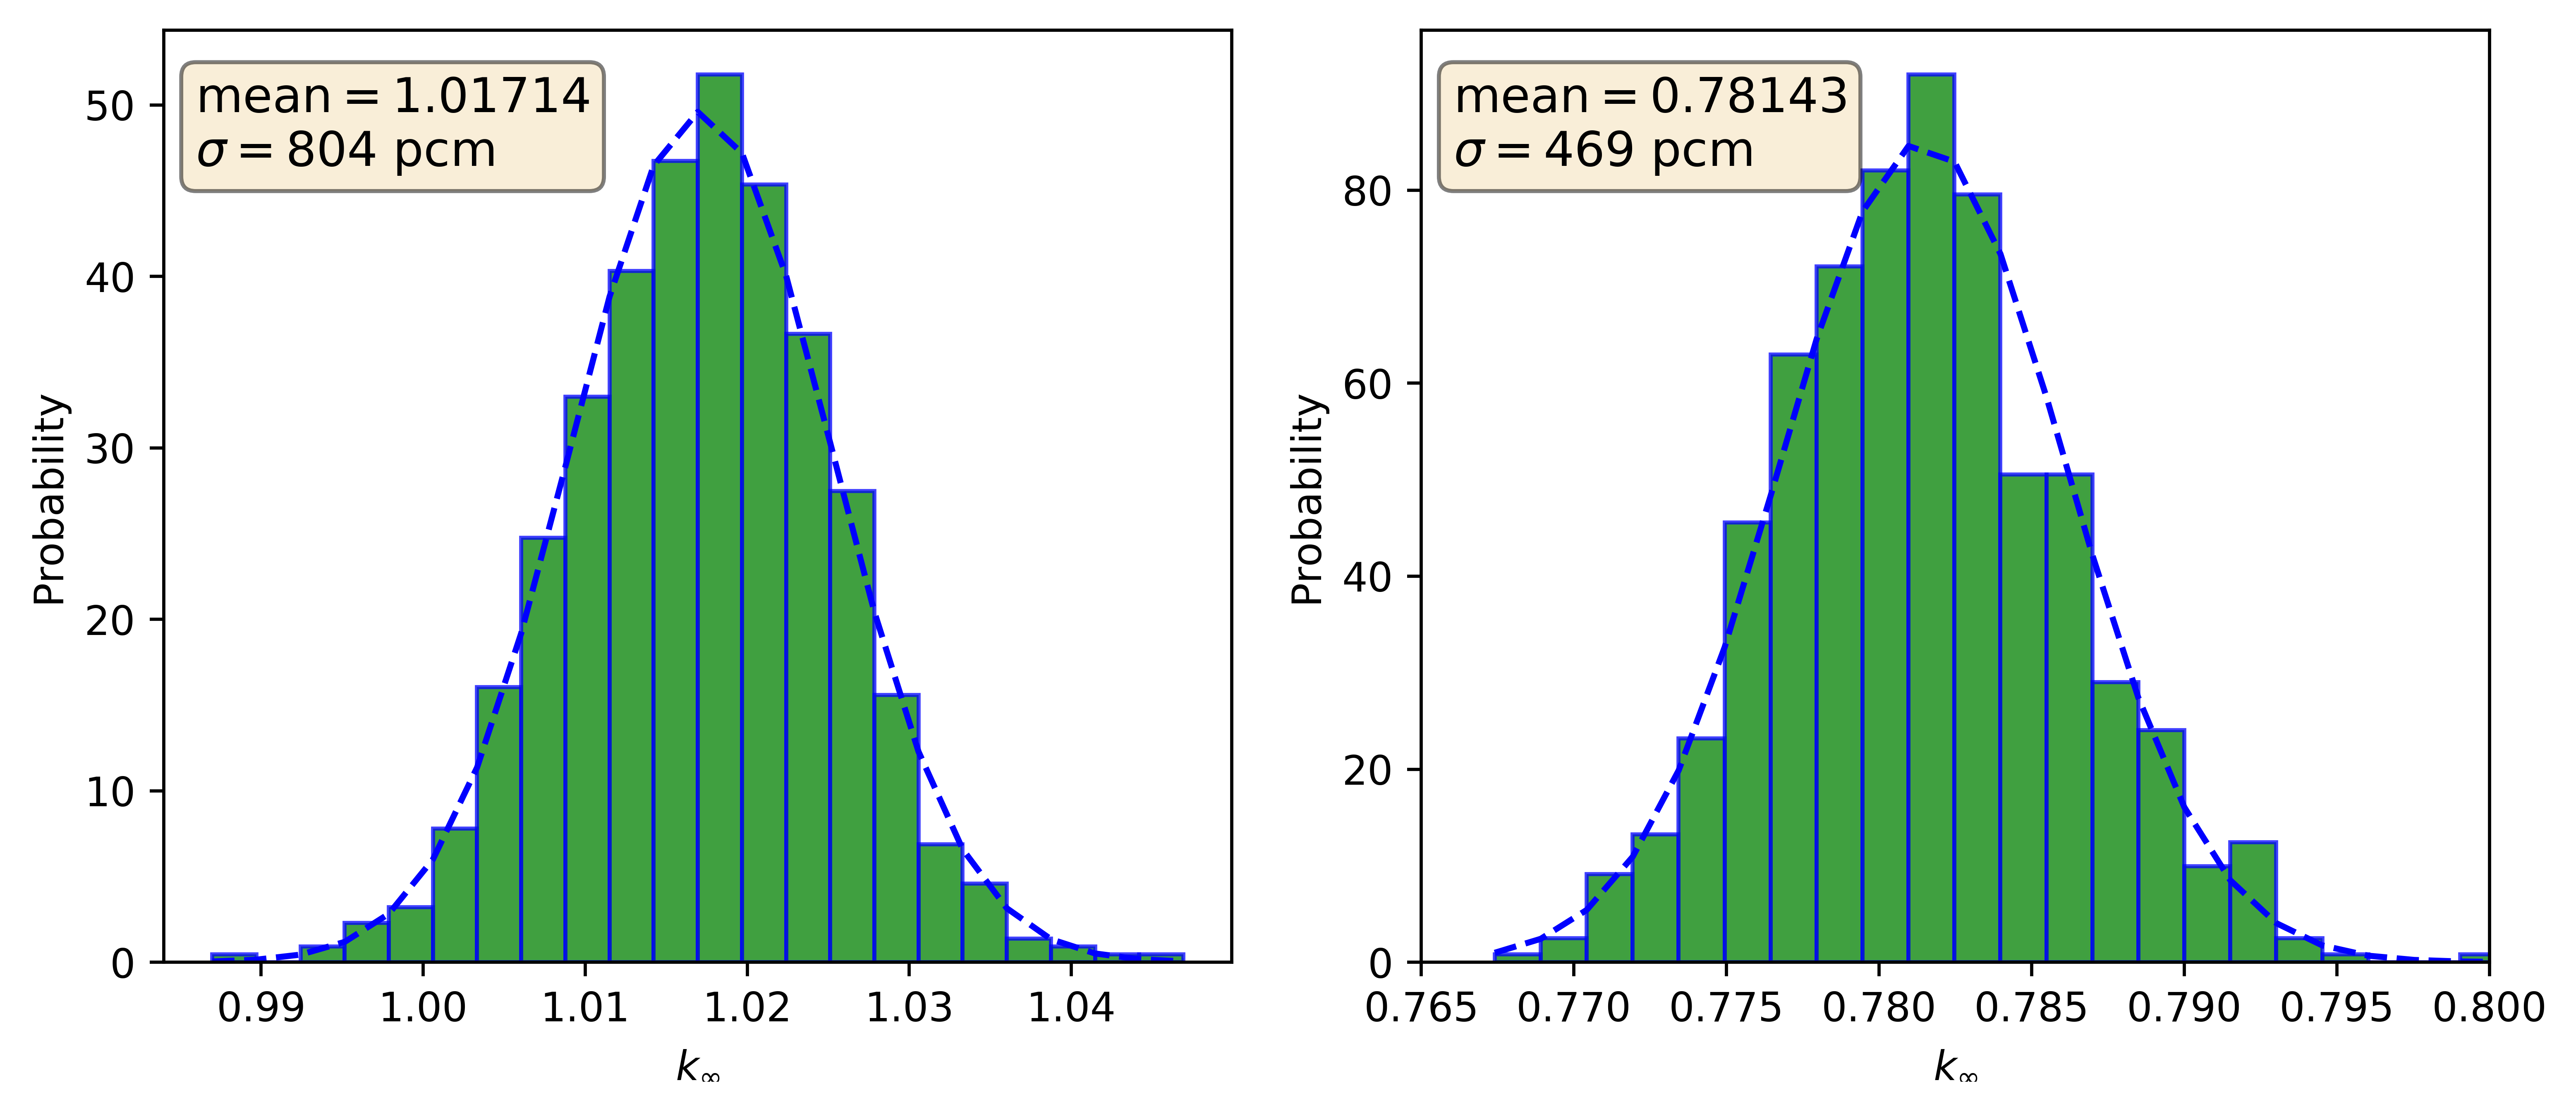
\includegraphics[width=\textwidth]{uq/endf_scale_keff_hist_for_tap.png}
	\vspace{-8mm}
	\caption{Histograms of $k_{\infty}$ at the \gls{BOL} (left) and 
		\gls{EOL} (right) obtained with SCALE Sampler by stochastically 
		sampling the nuclear data (cross sections, fission yields, decay 
		constants).}
	\label{fig:uq-scale-kinf-hist}
\end{figure}
\begin{figure}[hbp!] % replace 't' with 'b' to 
	\centering
	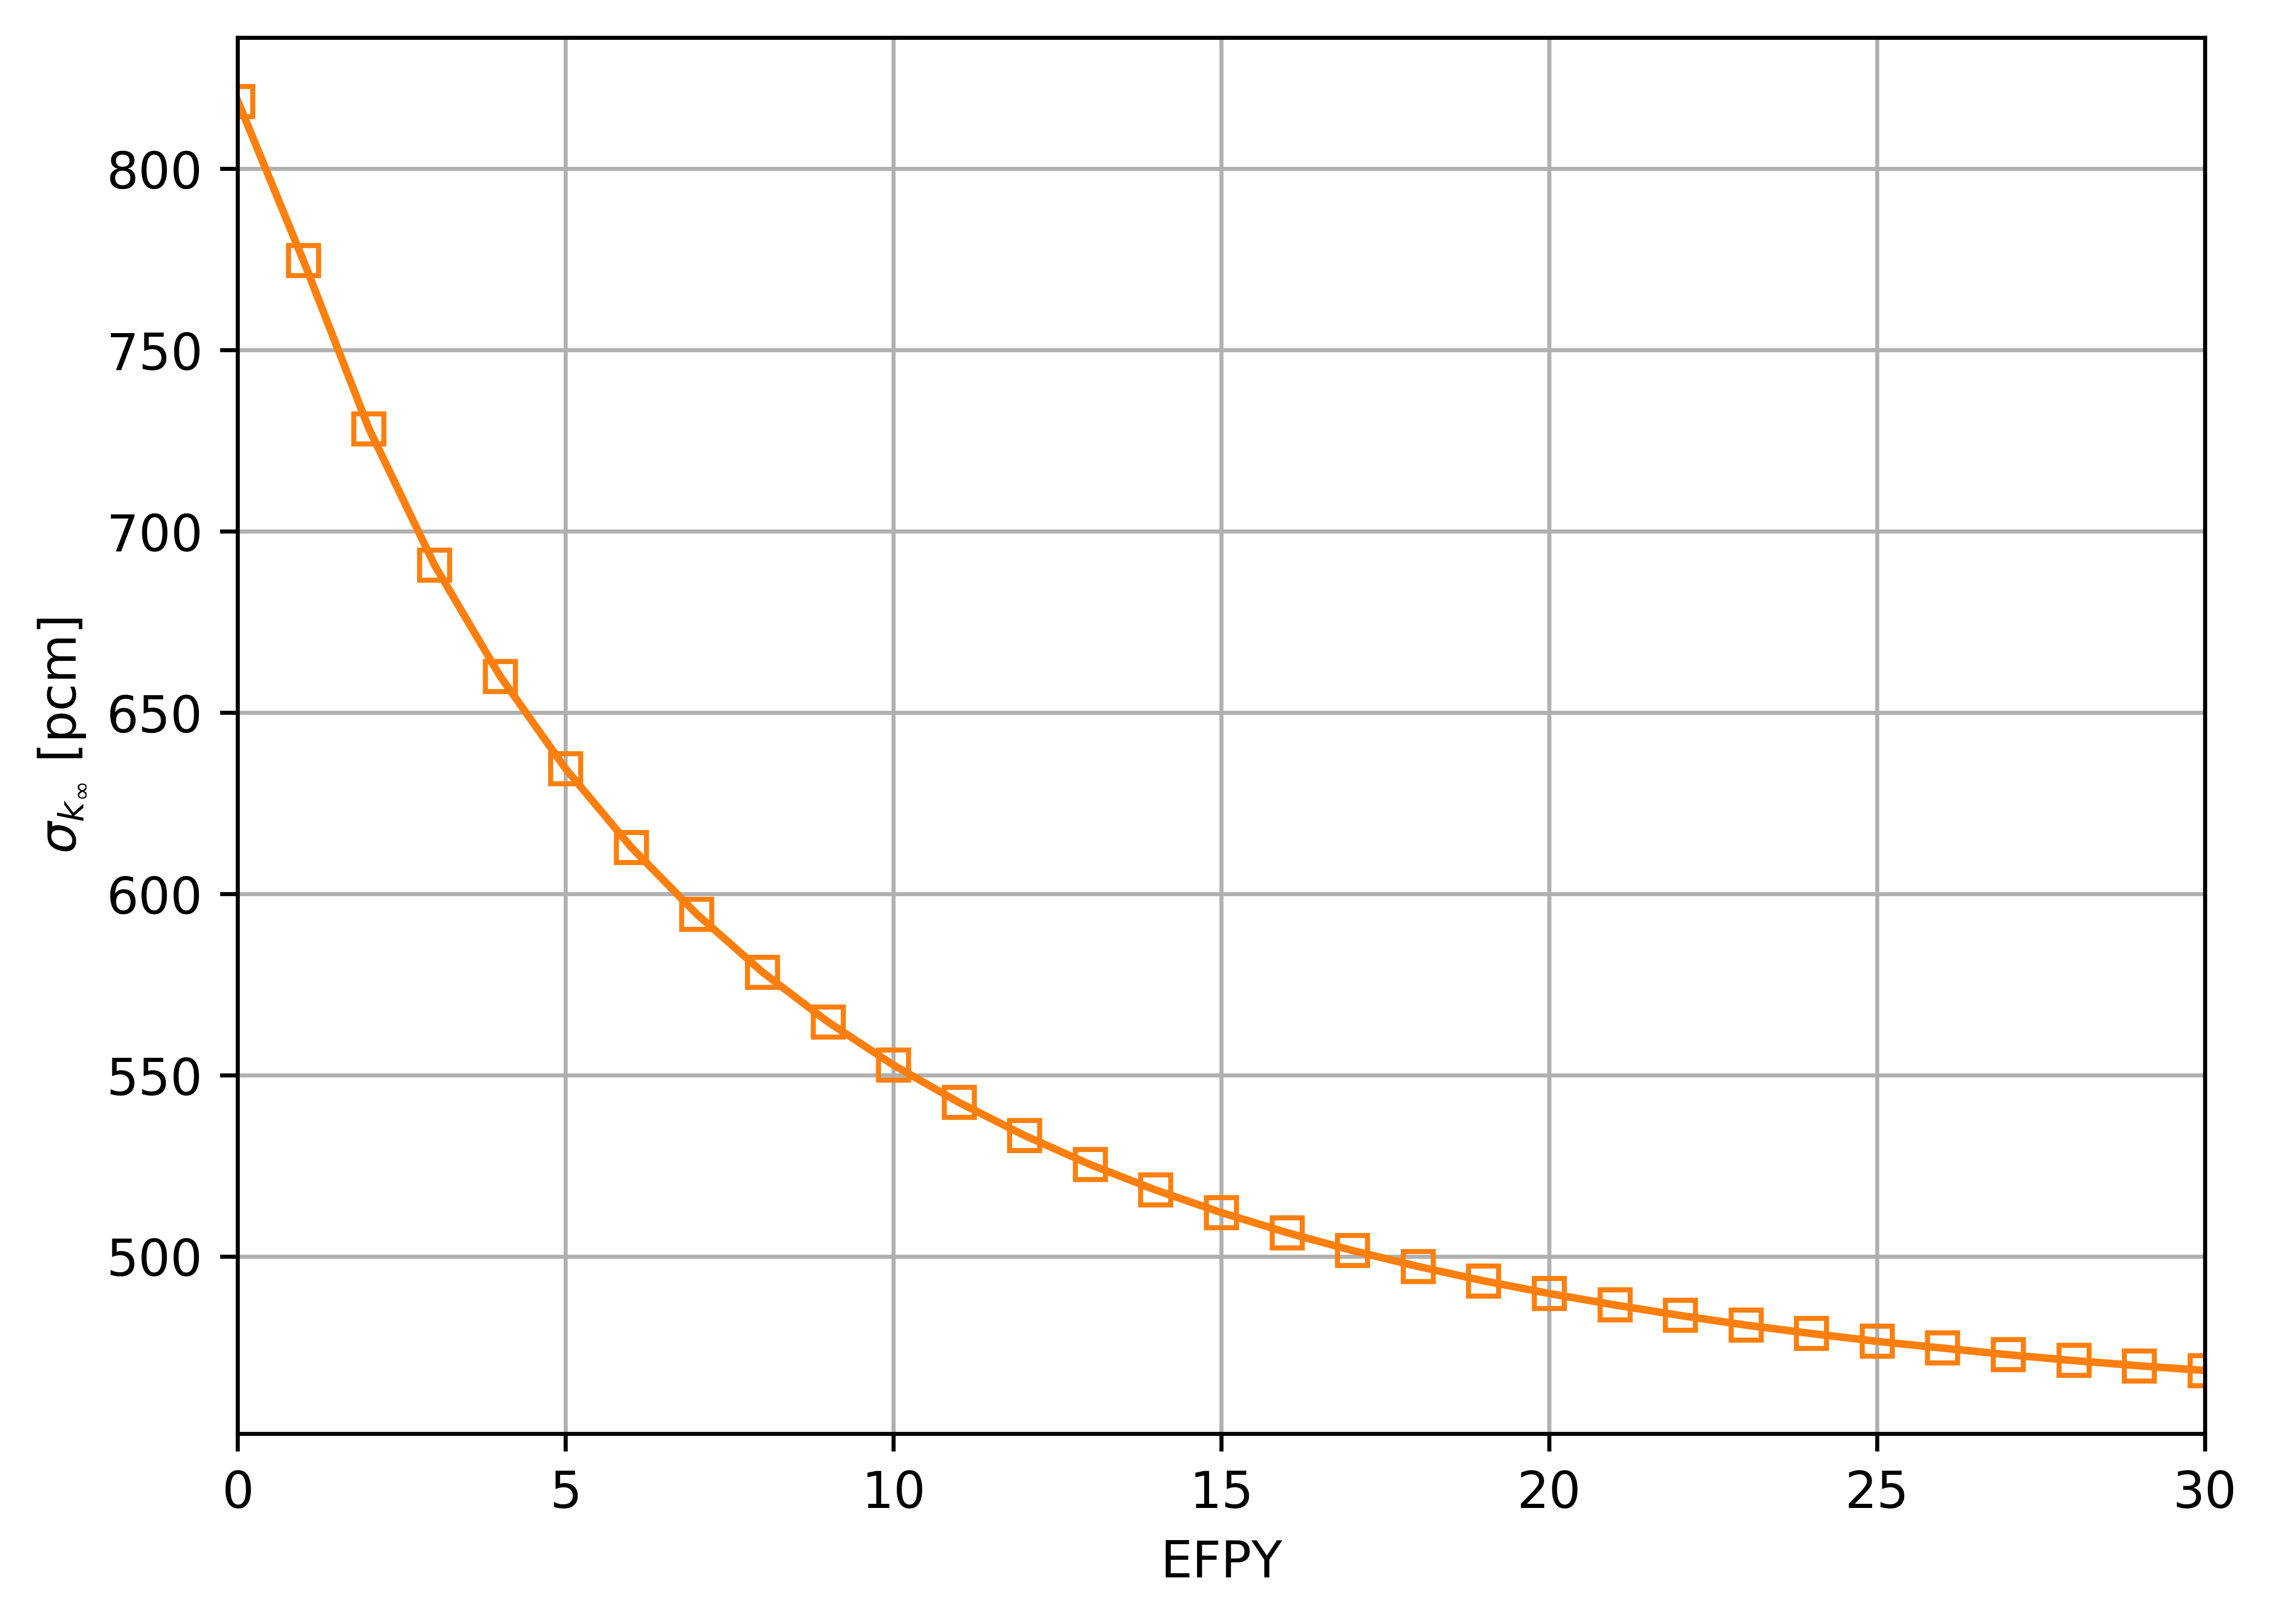
\includegraphics[width=\textwidth]{uq/scale_kinf_dynamics_for_tap.png}
	\caption{Calculated uncertainty in the infinite multiplication factor due 
		to the nuclear data uncertainty as a function of depletion time.}
	\label{fig:uq-scale-kinf}
\end{figure}

Figure~\ref{fig:uq-scale-kinf} demonstrates nuclear data-related uncertainty 
in the $k_{\infty}$ evolution during 30 years of operation. The $k_{\infty}$  
uncertainty decreased slowly because the $k_{\infty}$ mean value reduces over 
time from 1.01714 to 0.78143 due to fuel burnup. Considering more specific 
nuclear data contributions, at the \gls{BOL} the $k_{\infty}$ uncertainty is 
most likely to come from the fissile $^{235}$U fission ($n,f$) and neutron 
capture $(n,\gamma$) reaction cross sections; the $^{238}$U $(n,\gamma$) 
reaction cross section; and the elastic scattering cross section of hydrogen 
in zirconium hydride. However, moving toward the \gls{EOL}, the contributions 
to uncertainty from $^{235}$U data are expected to diminish due to the burnup 
and be substituted by the cross section uncertainties of the fissile plutonium 
(e.g., $^{239}$Pu, $^{241}$Pu). Notably, the $^{235}$U fission cross section 
uncertainty in intermediate and fast spectrum ranges (the \gls{TAP} is an
intermediate spectrum reactor, see Figure~\ref{fig:ben-spectrum-bol}) reaches 
up to 4\%, while it is less than 2.6\% for $^{239}$Pu and $^{241}$Pu. 
$^{239}$Pu and $^{241}$Pu capture and fission cross sections formed the 
dominant source of uncertainty after $^{235}$U was mostly depleted. 
%This $k_{\infty}$ 
%uncertainty evolution is in good agreement with results in the literature  
%\cite{rochman_nuclear_2014, radaideh_advanced_2019}. 

Moreover, the $k_{\infty}$ relative uncertainty from nuclear data slipped 
from 0.78\% at the \gls{BOL} to 0.46\% at the \gls{EOL}. This error is 
slightly larger than results in the literature for conventional \glspl{LWR} 
(e.g., 0.44\% \cite{williams_statistical_2013} or 0.55\% 
\cite{campolina_uncertainty_2018} for a \gls{PWR}). This discrepancy between 
$k_{\infty}$ uncertainty for the \gls{TAP} \gls{MSR} and \gls{PWR} likely 
originates with the $^{19}$F and $^{7}$Li nuclear data, which have significant 
covariances across reactions.

Figure~\ref{fig:uq-scale-u-pu} shows the standard deviations in uranium and 
plutonium isotopic inventory as a function of time. The uncertainty in 
$^{238}$U is minimal ($<0.1$\%) and almost constant with burnup because 
$^{238}$U mass does not change significantly from its initial inventory. The 
$^{236}$U uncertainty also is nearly constant during 30 years of operation and 
has a value of $\approx3.8$\%. However, $^{235}$U mass uncertainty increases 
steadily with burnup, due to its inventory decrease during 30 years of 
operation. The absolute mass uncertainty for $^{235}$U demonstrated growth 
from 5 kg at 1 year after startup to approximately 30 kg at the \gls{EOL}.

The uncertainty of major plutonium isotopes (e.g., $^{239}$Pu, $^{240}$Pu, 
$^{241}$Pu) is below 2\% over 30 years of burnup 
(Figure~\ref{fig:uq-scale-u-pu}, lower plot). The fissile $^{239}$Pu and 
poisonous $^{240}$Pu relative standard deviations are increased slightly from 
1.25\% to 1.6\% and from 1.65\% to 1.95\%, respectively. The relative standard 
deviation in fissile $^{241}$Pu mass is significant at the beginning of the 
operation, when its inventory is small (4 kg), and then decreases and 
approaches an equilibrium value of $\approx1.45$\% at the \gls{EOL}. The 
most significant relative standard deviation is observed for $^{242}$Pu mass 
($8.13$\%) because its concentration in fuel is minimal throughout 30 years 
of operation (Table~\ref{tab:uq-scale-mean-std-rsd}).
\begin{figure}[hbp!] % replace 't' with 'b' to 
	\centering
	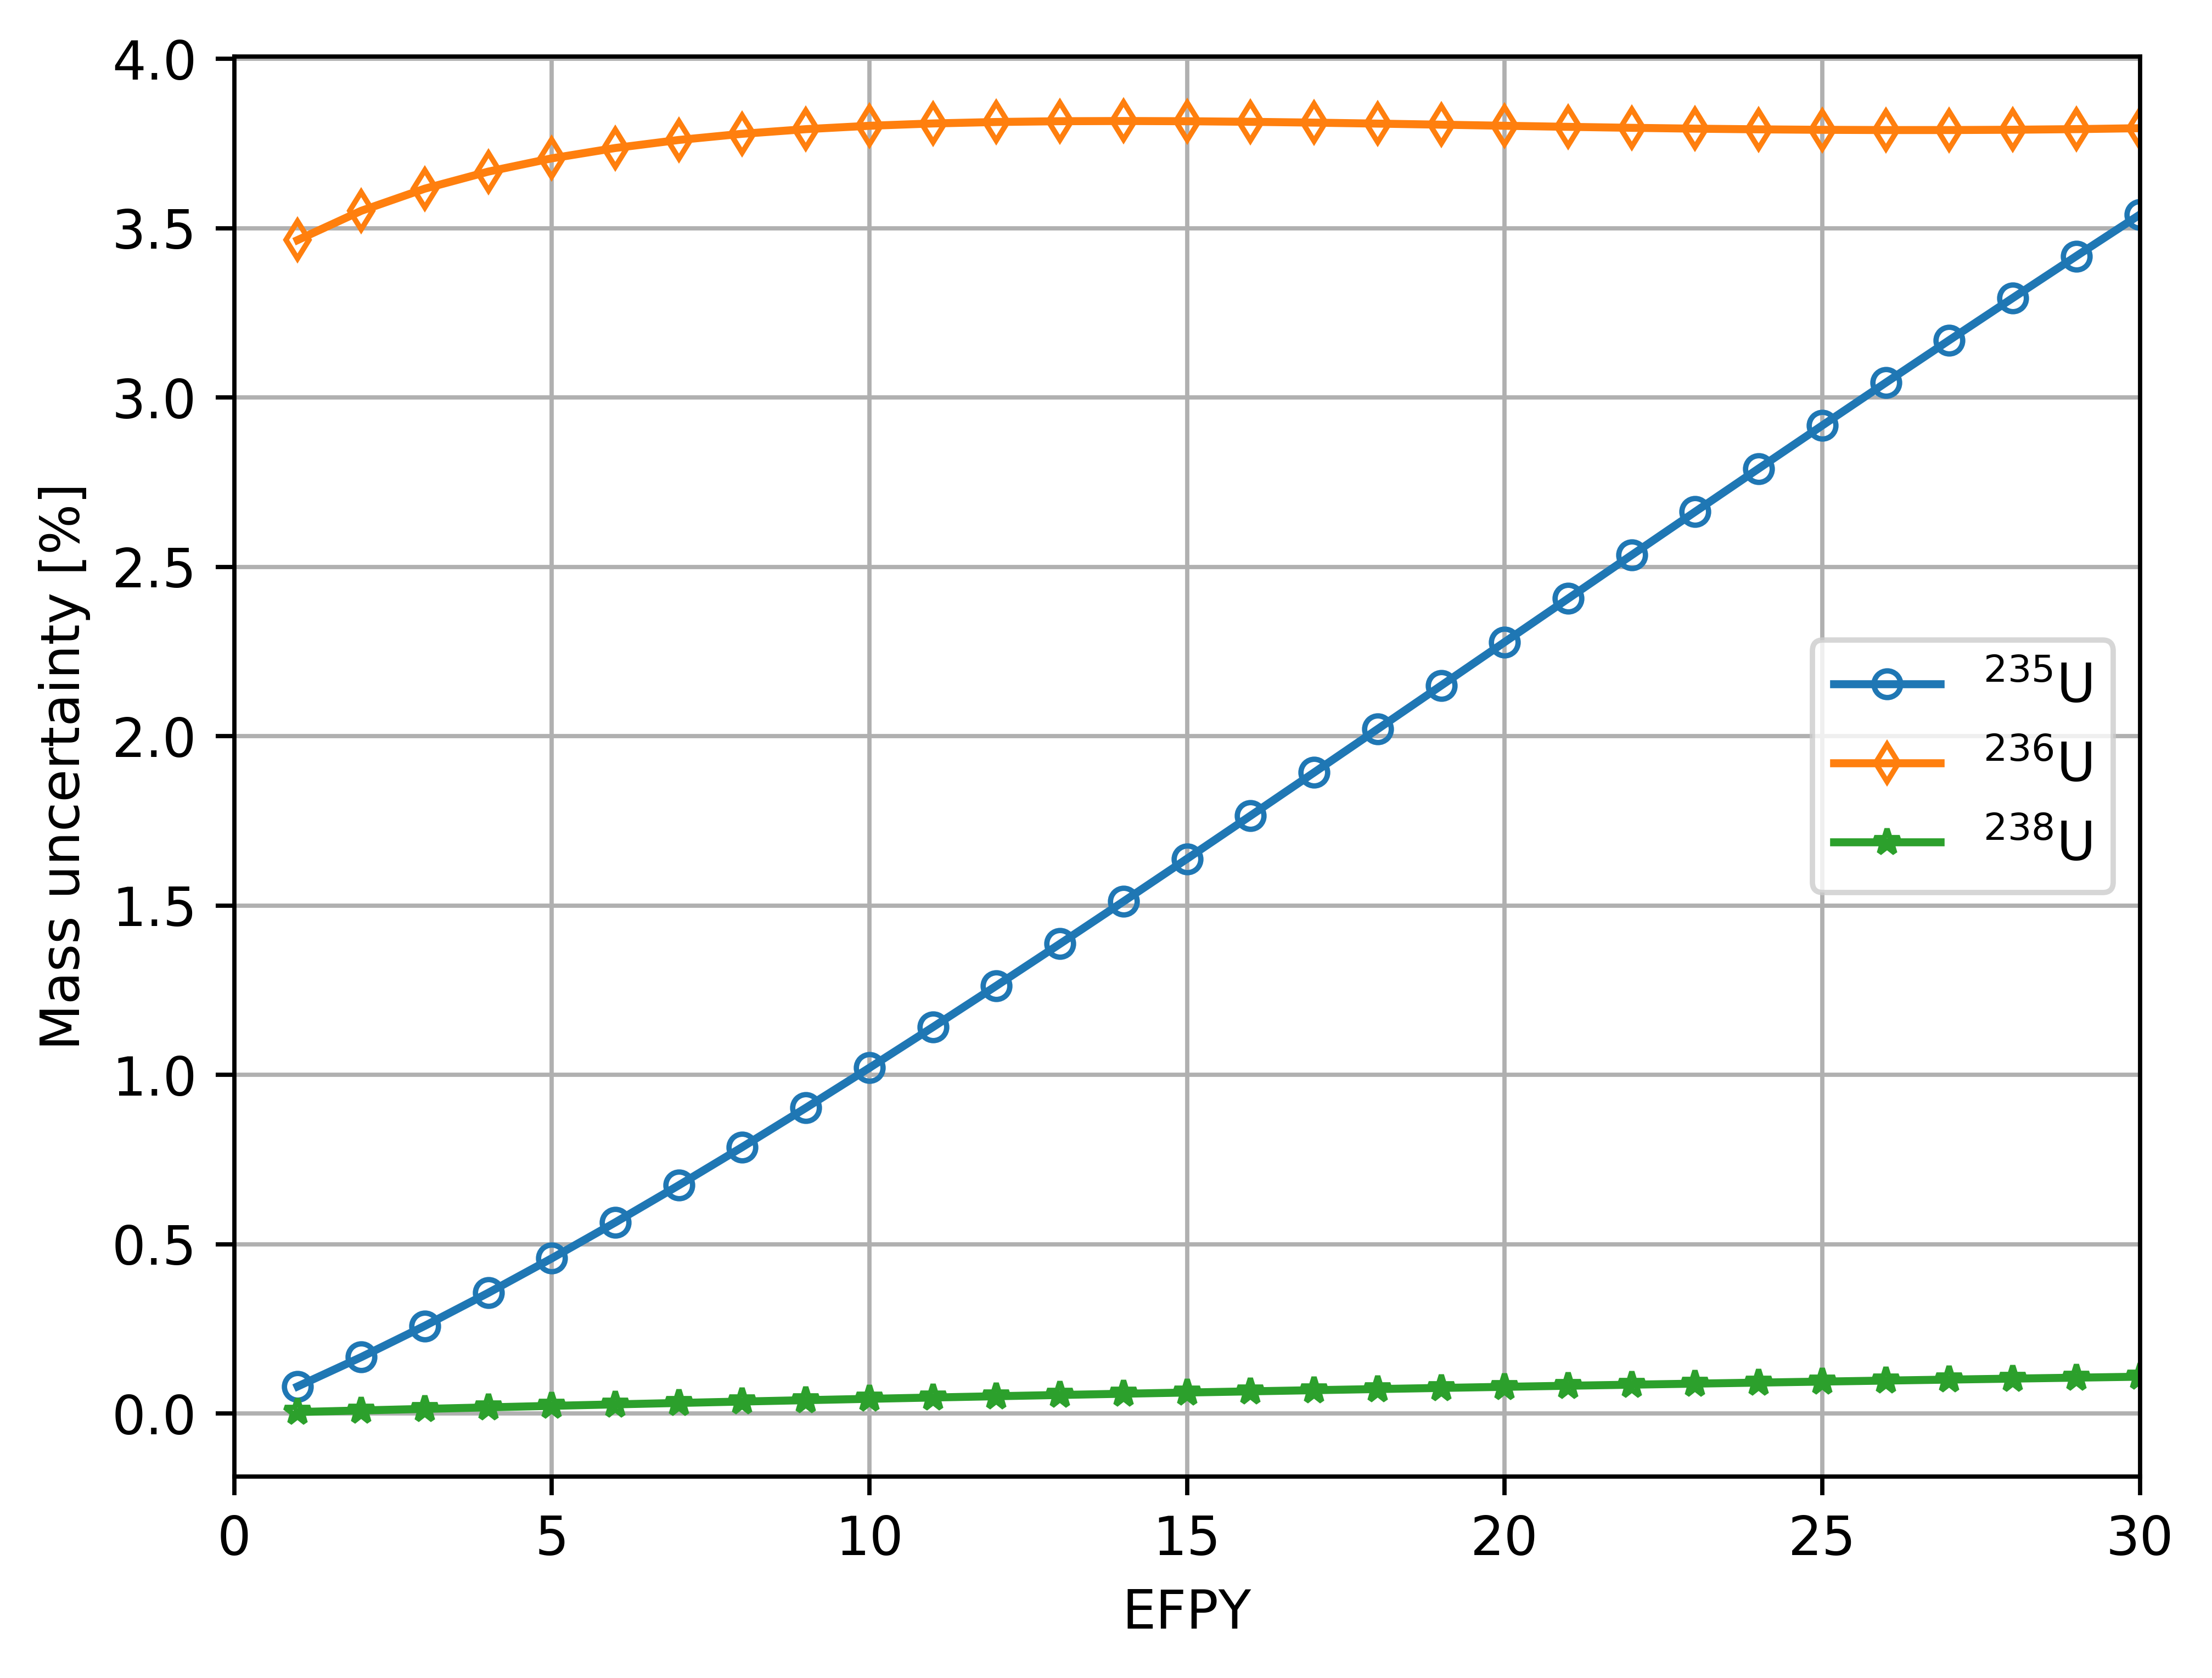
\includegraphics[width=0.85\textwidth]{uq/scale_mass_std_u.png}
	\vspace{-12mm}
	\hspace{0.0mm}
	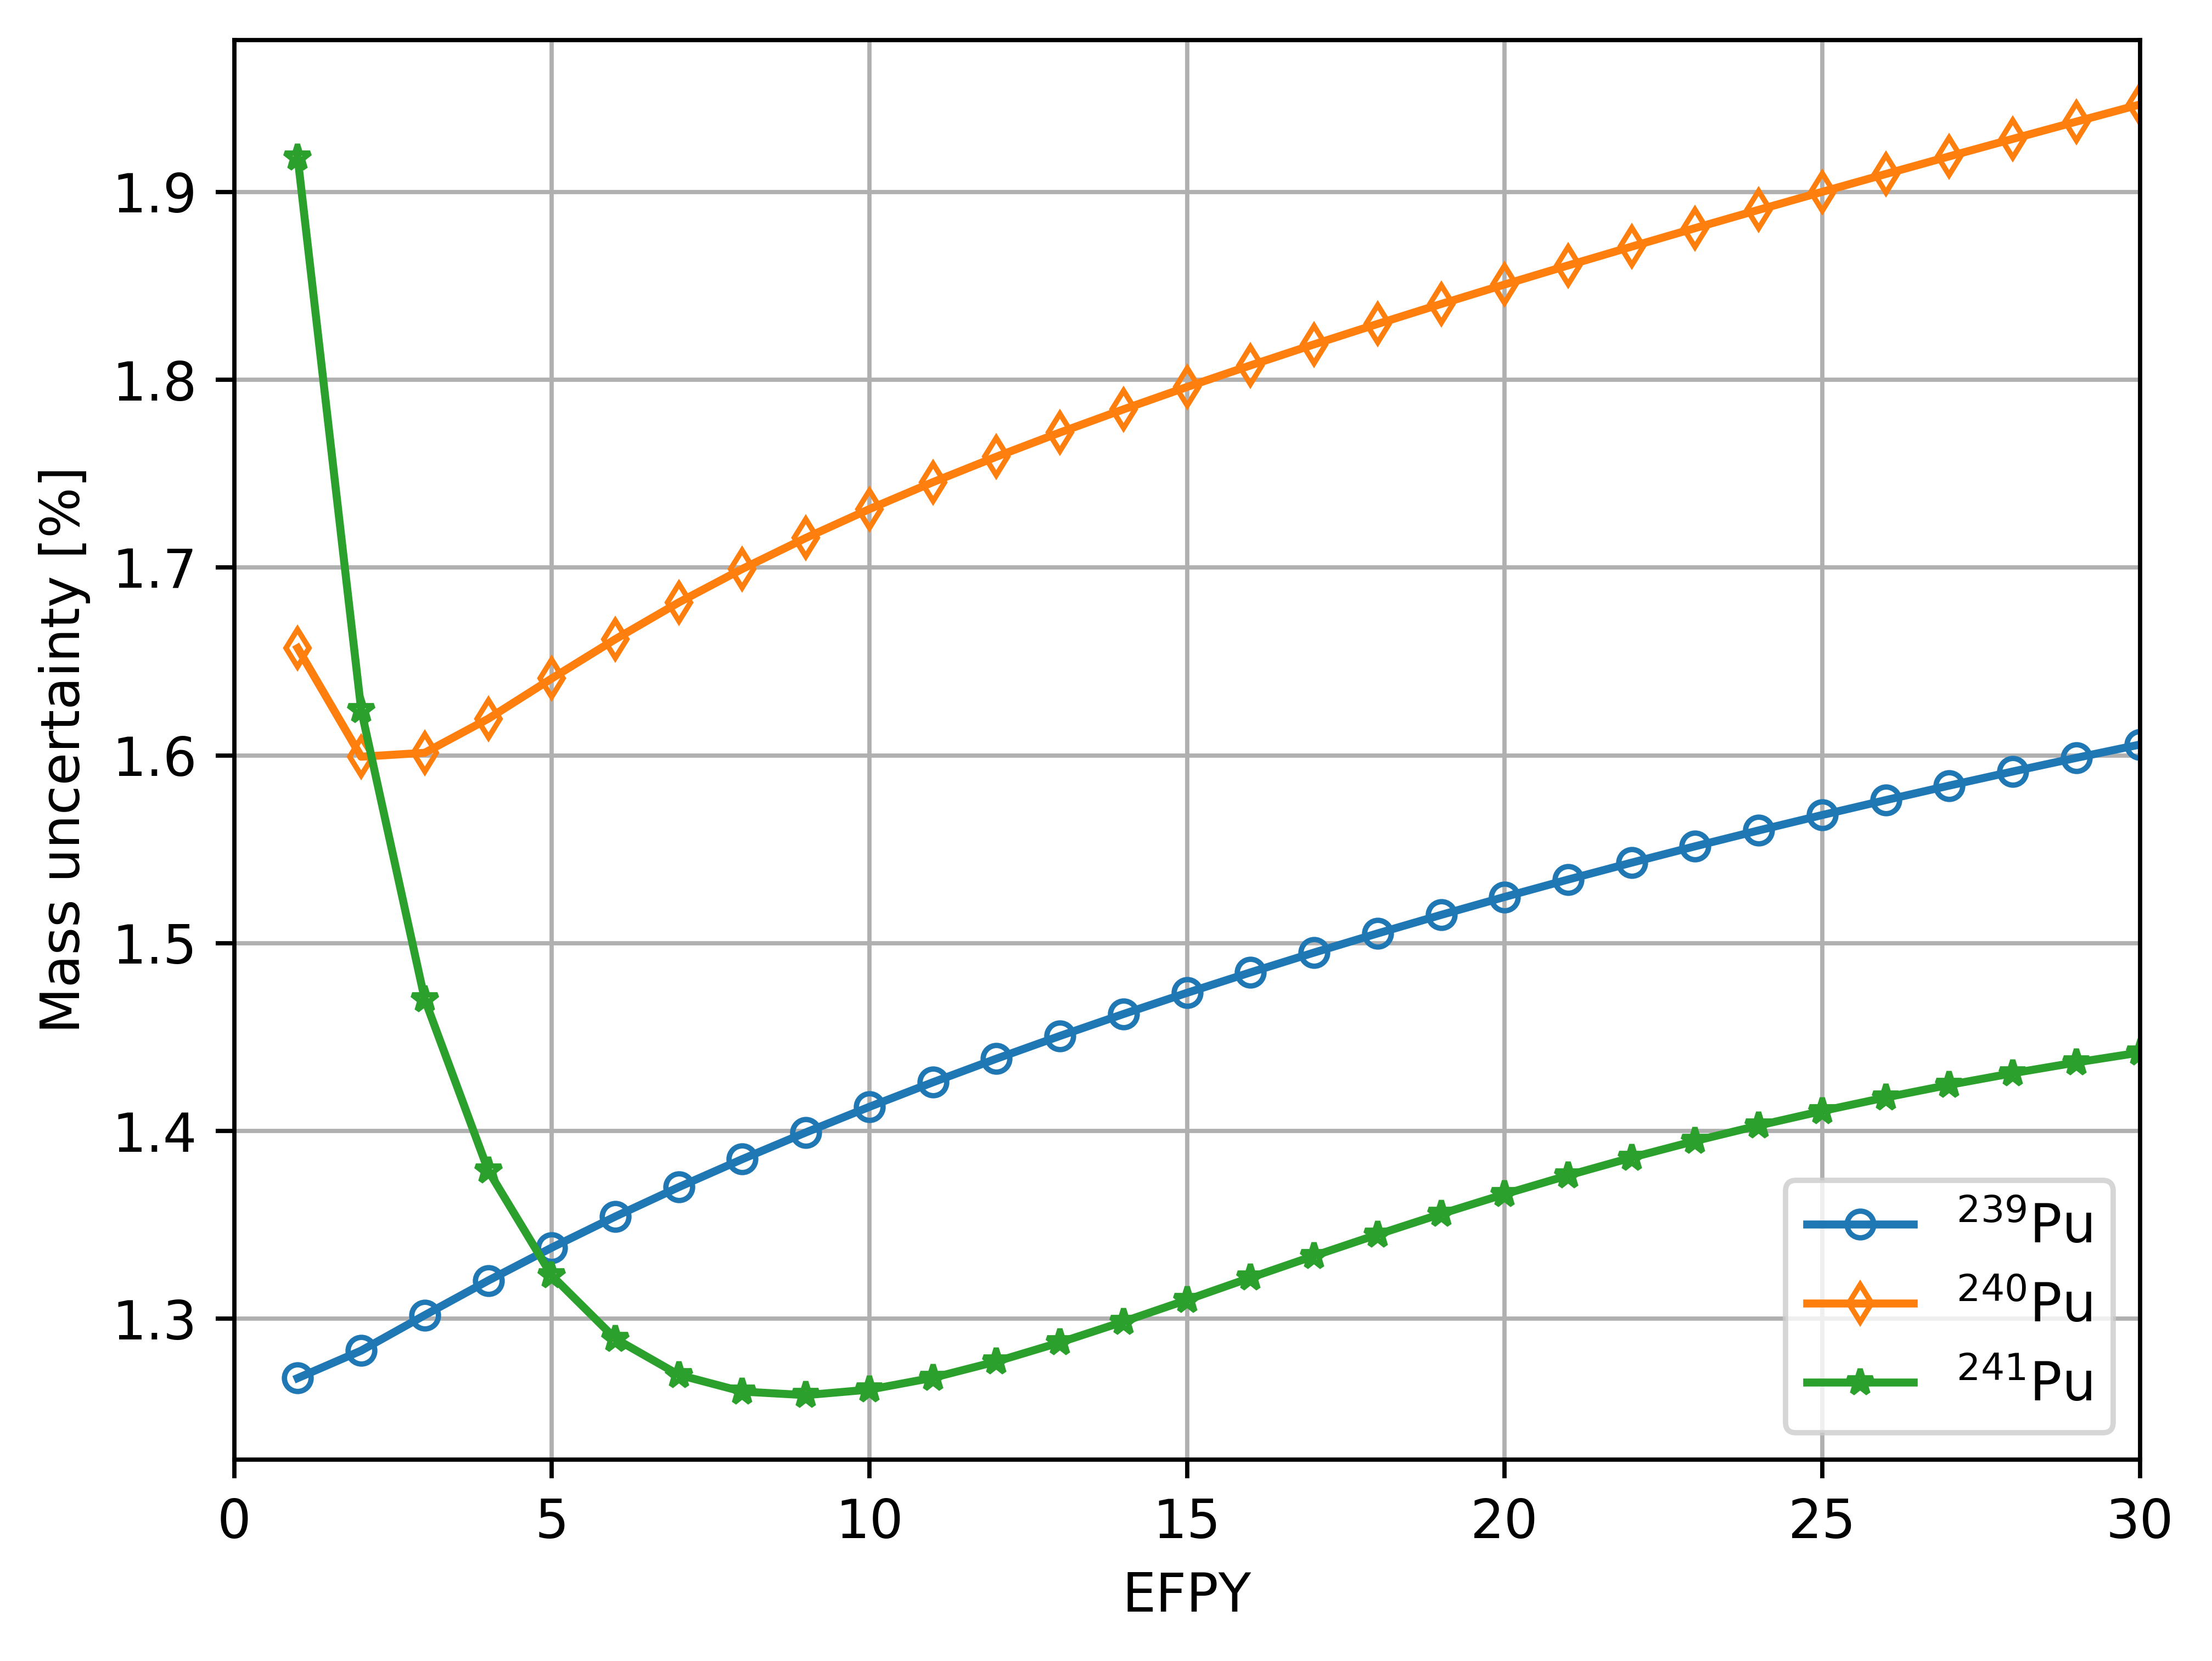
\includegraphics[width=0.85\textwidth]{uq/scale_mass_std_pu.png}
	\vspace{+8mm}
	\caption{Nuclear data-related uncertainty evolution in the uranium (upper) 
		and plutonium (lower) isotopic inventory during 30 years of depletion.}
	\label{fig:uq-scale-u-pu}
\end{figure}

Figure~\ref{fig:uq-scale-xe-i} shows the mass uncertainties for the selected 
\glspl{FP}: $^{135}$Xe and its primary direct precursor, $^{135}$I. The masses 
of $^{135}$Xe and $^{135}$I are in the ranges of 24-27 g and 18-19 g, 
respectively. As expected, relative standard deviations for these isotopes are 
relatively low due to minimal uncertainty of fission yield for $^{235}$U. The 
relative standard deviation of $^{135}$Xe mass changes in a range from 
0.47\% to 0.6\%, while the $^{135}$I standard deviation ranges from 0.35\% to 
0.56\%.
\begin{figure}[hbp!] % replace 't' with 'b' to 
	\centering
	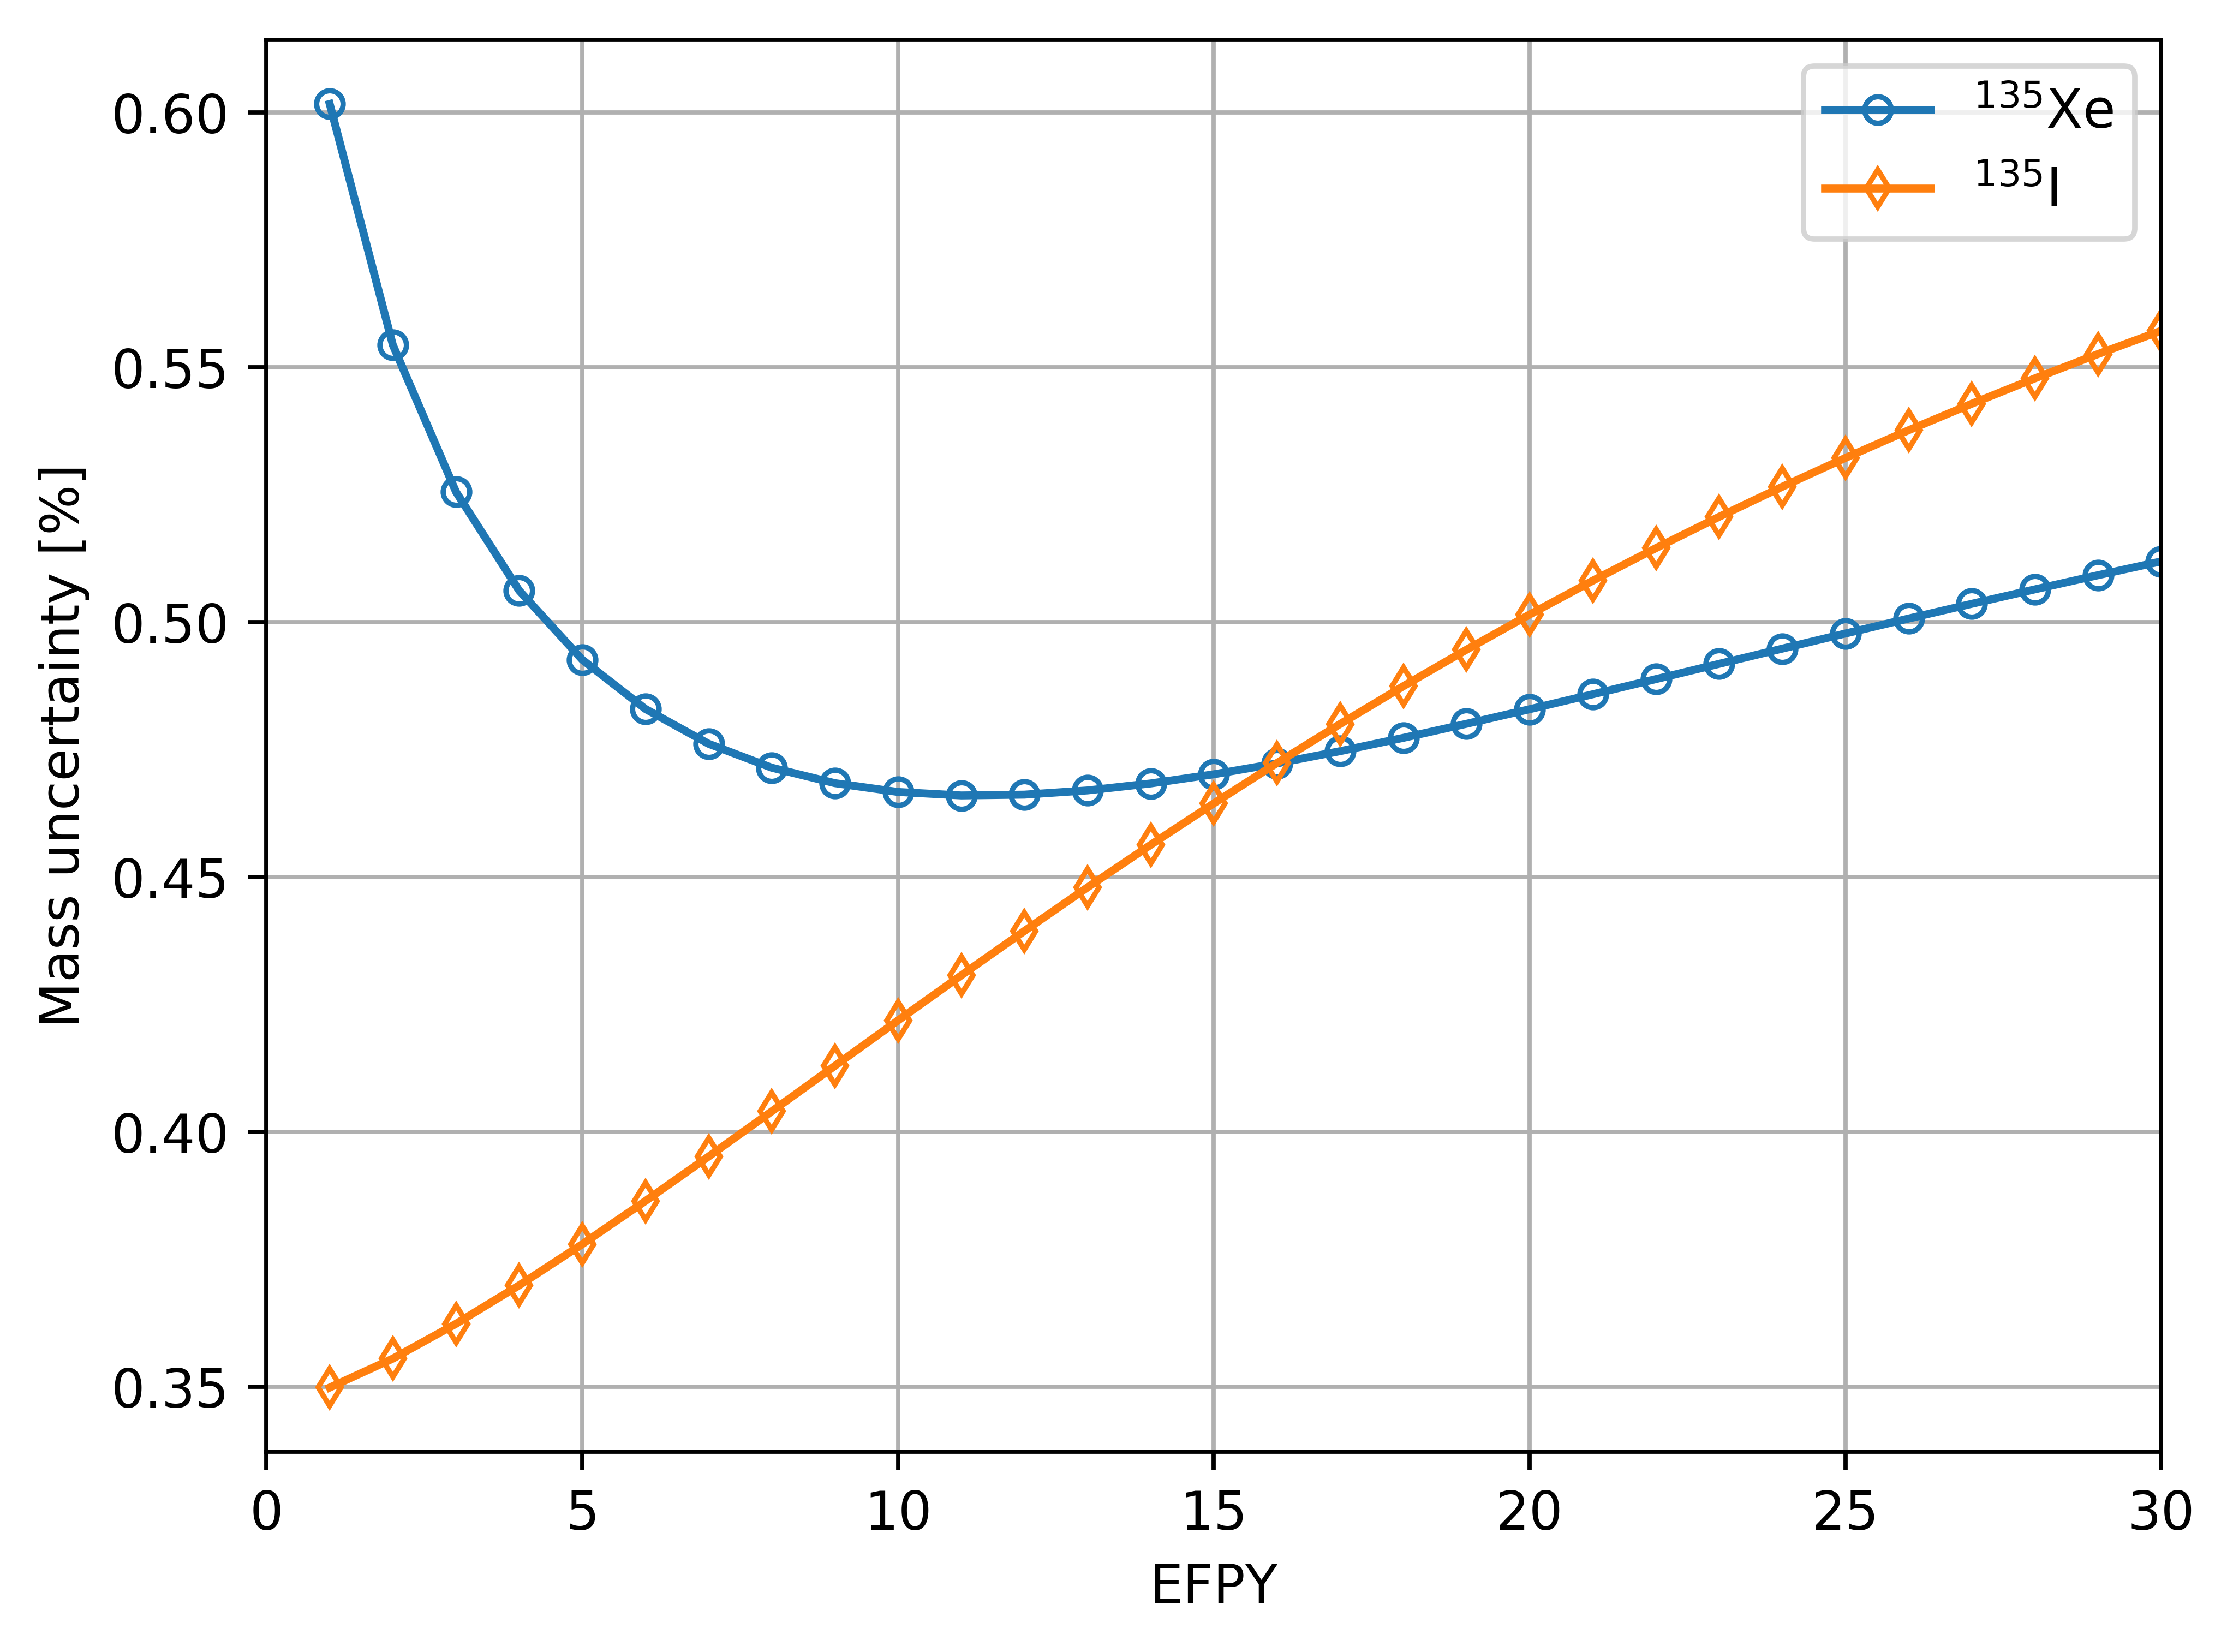
\includegraphics[width=0.85\textwidth]{uq/scale_mass_std_xe_i.png}
	\caption{Nuclear data-related uncertainty evolution in $^{135}$Xe and 
		$^{135}$I isotopic inventory during 30 years of depletion.}
	\label{fig:uq-scale-xe-i}
\end{figure}

Table~\ref{tab:uq-scale-mean-std-rsd} summarizes the nuclear data-related 
uncertainty in the isotopic inventory for the \gls{TAP} \gls{MSR} after 30 
years of operation. Overall, the mass uncertainties due to nuclear data 
uncertainties are two orders of magnitude larger than uncertainty due to 
the statistical error in \gls{MC}.  

All results presented in this section are based on 800 random samples obtained 
using the Sampler tool in SCALE. Figure~\ref{fig:uq-scale-convergence} 
shows the convergence of $k_{\infty}$ and $^{235}$U mass uncertainty with 
number of random samples. Notably, after 500 samples the $k_{\infty}$ and 
$^{235}$U mass uncertainties stabilize. Overall, 500 random samples is 
enough to accurately estimate uncertainty in the isotopic inventory due to 
uncertainty in nuclear data. 

%%%%%%%%%%%%%%%%%%%%%%%%%%%%%%%%%%%%%%%%
\begin{table}[hbp!]
	\centering
	\caption{Mean value, Standard Deviation (STD), and Relative Standard 
		Deviation (RSD) of mass for the major isotopes after 30-year depletion 
		analysis for the \gls{TAP} reactor. Only nuclear data-related 
		uncertainty is considered.}
	\begin{tabularx}{0.7\textwidth}{L R R R R}
		\hline
		\textbf{Isotope}  & \textbf{Mean [kg]} & \textbf{STD [kg]} & 
		\textbf{RSD [\%]}\\ \hline
		$^{234}$U  & 21.6  & 0.75  & 3.48\% \\
		$^{235}$U  & 839.4 & 29.72 & 3.54\% \\
		$^{236}$U  & 1154.9& 43.83 & 3.79\% \\
		$^{238}$U  & 112,206.1 & 122.32 & 0.11\% \\
		$^{238}$Pu & 335.56& 11.05 & 3.29\% \\
		$^{239}$Pu & 5558.1& 89.25 & 1.61\% \\
		$^{240}$Pu & 1594.6& 31.04 & 1.95\% \\
		$^{241}$Pu & 639.1 & 9.21  & 1.44\% \\
		$^{242}$Pu & 164.0 & 13.33 & 8.13\% \\
		$^{241}$Am & 204.9 & 6.15  & 3.00\% \\
		$^{135}$Xe & 0.03  &$<0.01$& 0.51\% \\
		$^{135}$I  & 0.02  &$<0.01$& 0.56\% \\ \hline
	\end{tabularx}
	\label{tab:uq-scale-mean-std-rsd}
	\vspace{-0.9em}
\end{table}
%%%%%%%%%%%%%%%%%%%%%%%%%%%%%%%%%%%%%%%%%%%%%%%%%%%%%%%%%%%%%%%%%%%%%%%%%%%%%%%


\begin{figure}[hbp!] % replace 't' with 'b' to 
	\centering
	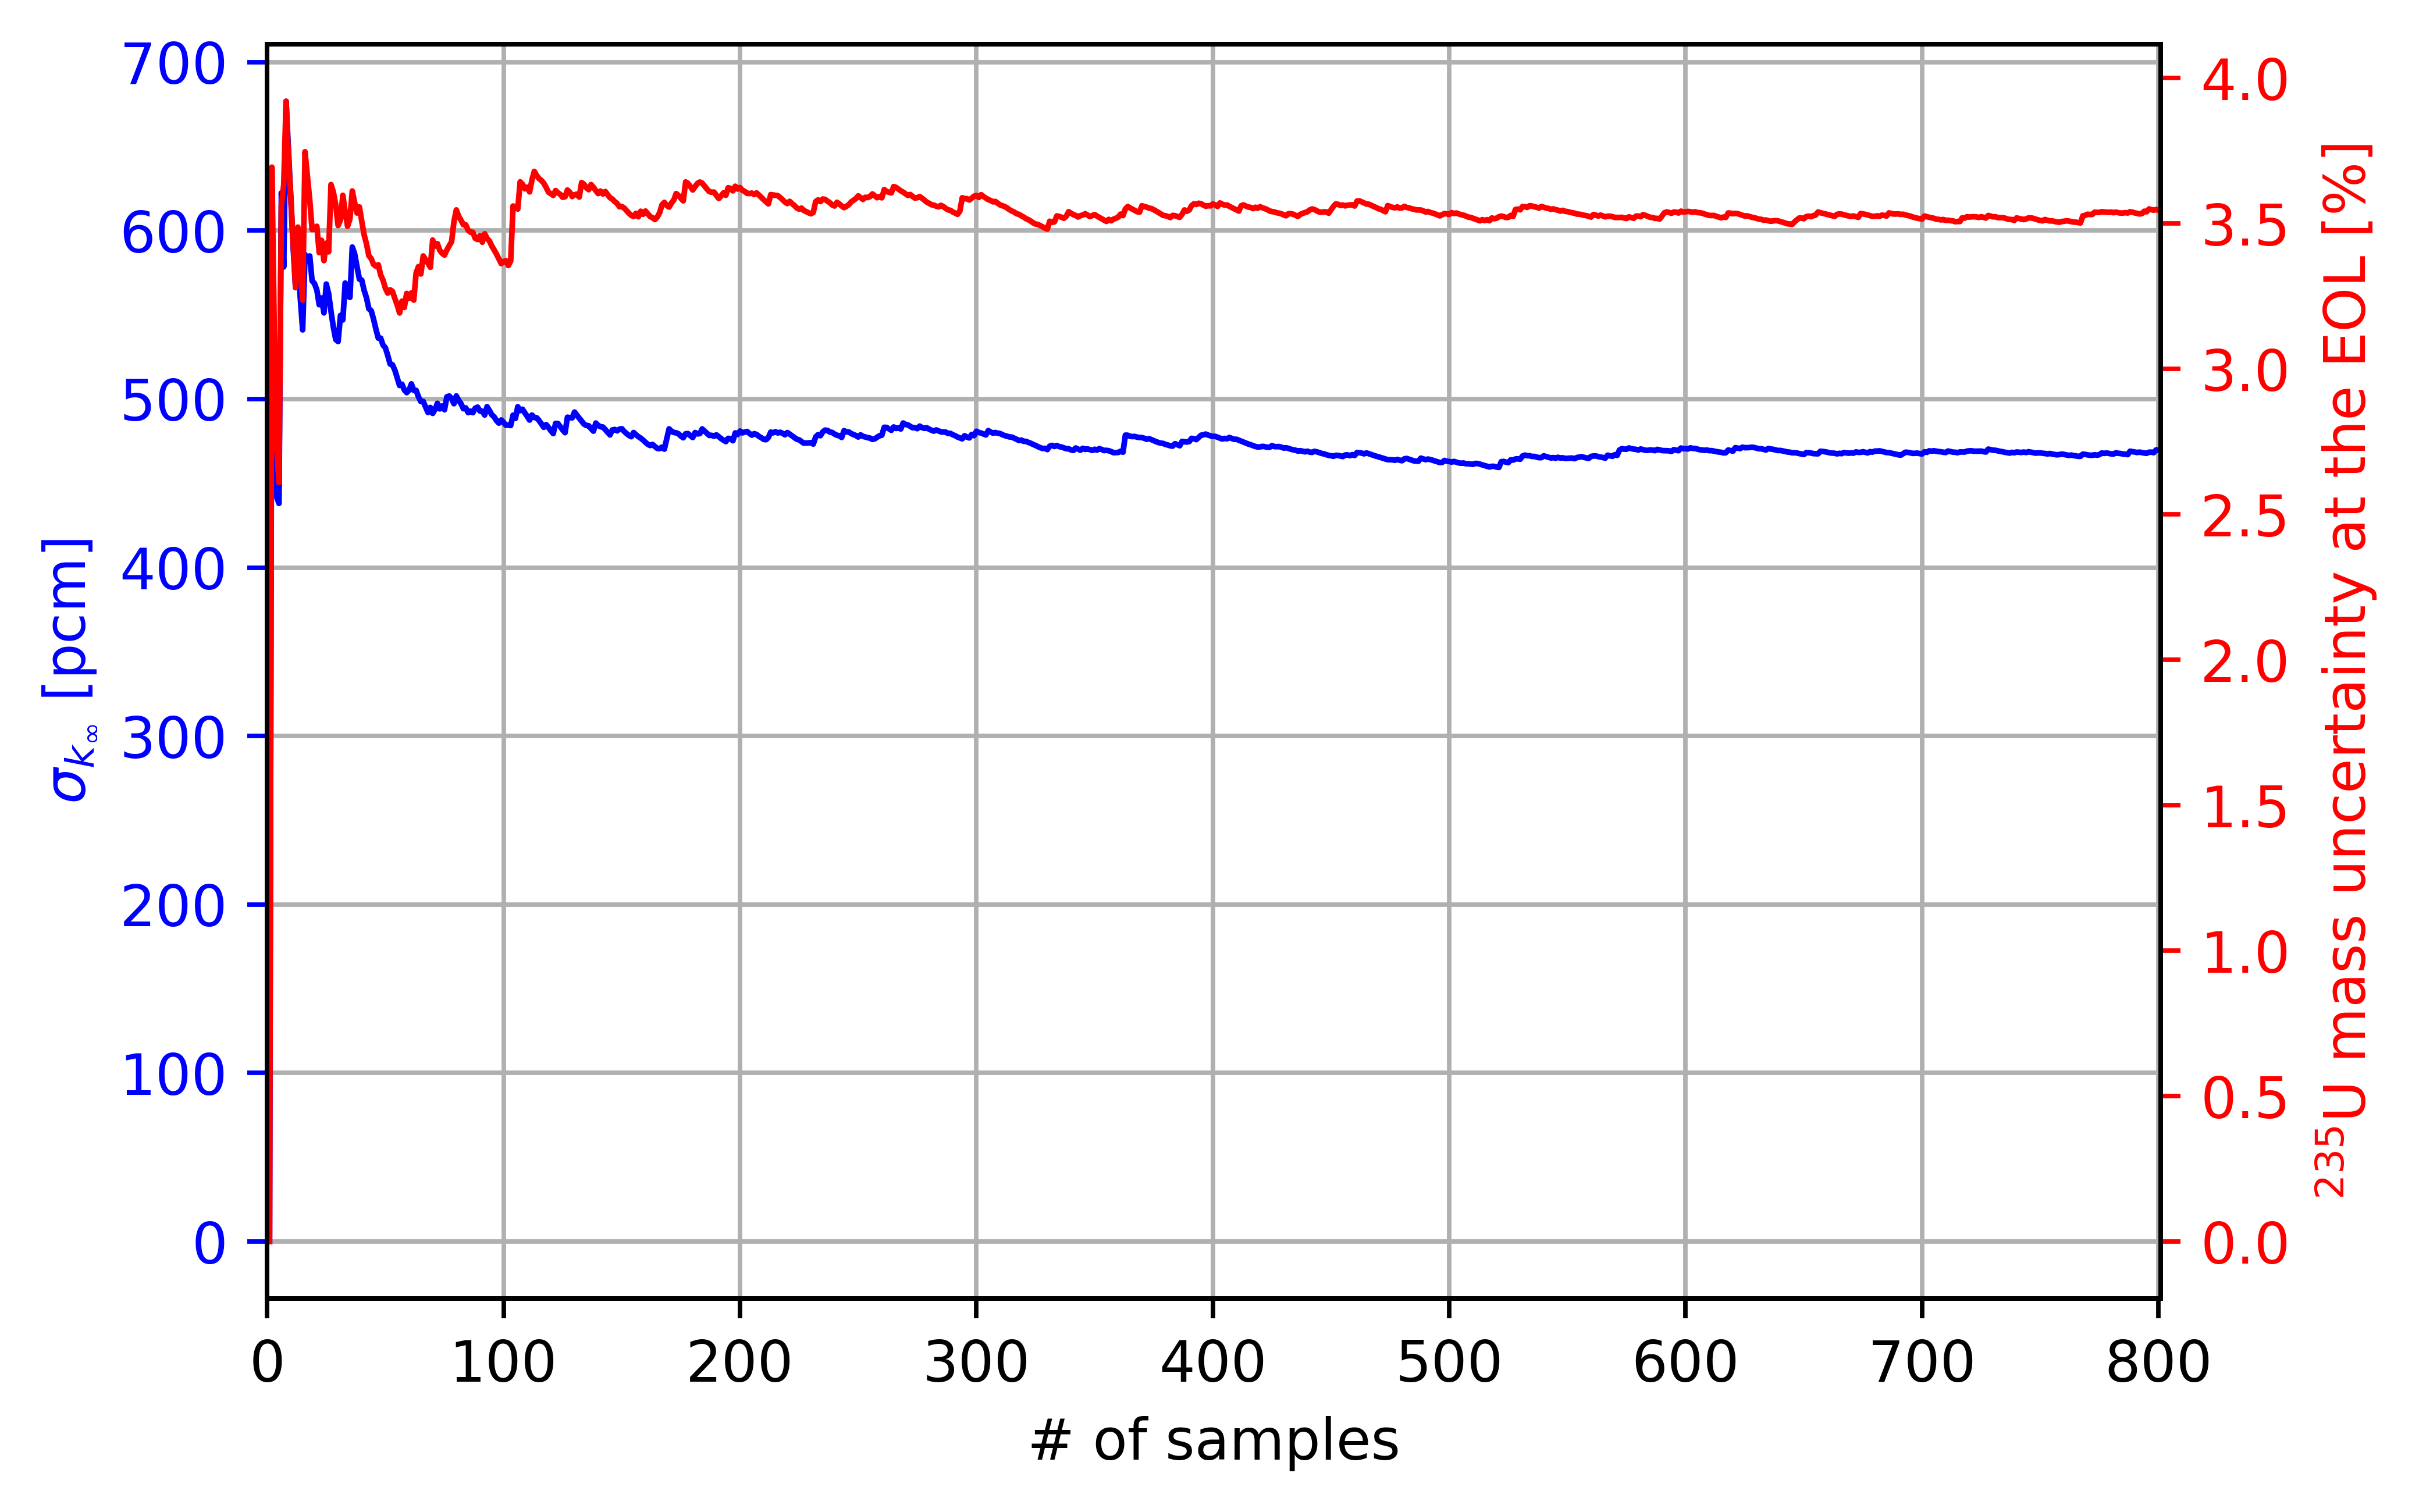
\includegraphics[width=\textwidth]{uq/scale_convergance_for_tap.png}
	\caption{Convergence of $k_{\infty}$ and $^{235}$U mass uncertainties due 
		to the nuclear data uncertainty as a function of the number of samples 
		for 
		simulation using SCALE with the Sampler module.}
	\label{fig:uq-scale-convergence}
\end{figure}

\section{Concluding remarks}
Uncertainty propagation analysis was performed for the depletion calculation 
for the \gls{TAP} \gls{MSR} 30-year burnup. I separately considered two 
primary sources of uncertainty in the depletion calculations: stochastic 
uncertainty in the neutron flux distribution and uncertainty in the nuclear 
data. Stochastic error in the isotopic composition was obtained using the 
Serpent Continuous Energy Monte Carlo code by running the same depletion 
sequence 1000 times, each time with a new initial random seed. The 
Sampler module in SCALE 6.2 with a 56-group covariance library was used to 
obtain nuclear data-related uncertainty in the isotopic composition of the 
fuel salt. 
Uncertainties in the input nuclear data (cross sections, fission yields, decay 
constants) are propagated throughout all steps of the transport/depletion 
sequence, including self-shielding, space-energy flux calculation, and isotope 
transmutation. 

The stochastic errors in isotopic masses are below 0.067\% 
for 7.5 million neutron histories (total neutron flux relative stochastic 
error $<0.01$\%). Therefore, it is unnecessary to consider the accumulation of 
the stochastic error for the fuel depletion in the \gls{TAP} reactor 
considered in this dissertation.
Finally, the stochastic error in the isotopic inventory could be reduced to 
almost zero by increasing the number of neutron histories, but it is 
impractical due to the sublinear convergence rate of the Monte Carlo method 
($O(\sqrt{N})$).

On the other hand, the computed errors in the isotopic inventory due to the 
nuclear data uncertainties are a few orders of magnitude larger and cannot 
be ignored. The nuclear data-related errors are in the range from 1\% to 2\% 
for the masses of $^{239}$Pu, $^{240}$Pu, and $^{241}$Pu, and about 3-8\% for  
$^{234}$U, $^{235}$U, $^{236}$U, $^{238}$Pu, $^{242}$Pu, and $^{241}$Am. 
Finally, the mass uncertainty for the selected \glspl{FP} ($^{135}$Xe and 
$^{135}$I), which are the subject of interest of the current work, is below 
0.6\%. Overall, the principal source of uncertainty in depletion calculations 
arises from to the nuclear data covariances.

Finally, this chapter demonstrated that the standard deviation in the 
multiplication factor due to the nuclear data uncertainty ranges from 804 to 
469 $pcm$, while the stochastic error is only about 30 $pcm$. Overall, to 
accurately capture the isotopic inventory evolution for the \gls{TAP} concept 
using SaltProc v1.0 with Serpent Monte Carlo code, it is unnecessary to 
waste a vast computational power to simulate $10^7-10^9$ neutron histories per 
each depletion step because the impact of the stochastic errors in 
neutron fluxes is negligible compared with the nuclear data-related errors.
\FloatBarrier
%\section{Methods}

The ability of liquid-fueled systems to continuously remove fission products and add 
fissile and/or fertile elements is the main challenge for depletion simulations. 
The python package introduced in this work, SaltProc, takes into account online 
separations and feeds using the SERPENT 2 continuous-energy Monte Carlo neutron 
transport and depletion code. In this work, all figures of the core model
were generated using the built-in SERPENT 2 plotter. 

\subsection{Molten Salt Breeder Reactor design and model description}
The \gls{MSBR} vessel has a diameter of 680 cm and a height of 610 cm. It 
contains a molten fluoride fuel-salt mixture that generates heat in the active 
core region and transports that heat to the primary heat exchanger by way of 
the primary salt pump. In the active core region, the fuel salt flows through 
channels in moderating and reflecting graphite blocks. Fuel salt at
565$^{\circ}$C enters the central manifold at the bottom via four 
40.64-cm-diameter nozzles and flows upward through channels in the lower plenum 
graphite. The fuel salt exits at the top at about 704$^{\circ}$C through four 
equally spaced nozzles which connect to the salt-suction pipes leading to 
primary circulation pumps. The fuel salt drain lines connect to the bottom of 
the reactor vessel inlet manifold.

Figure~\ref{fig:serpent_plan_view} shows the configuration of the 
\gls{MSBR} vessel, including the ``fission" (zone I) and ``breeding" 
(zone II) regions inside the vessel. The core has two radial zones bounded by a 
solid cylindrical graphite reflector and the vessel wall. The central zone, 
zone I, in which 13\% of the volume is fuel salt and 87\% graphite, is
composed of 1,320 graphite cells, 2 graphite control rods, and 2 
safety\footnote{ These rods needed for emergency shutdown only.} rods. The 
under-moderated zone, zone II, with 37\% fuel salt, and radial reflector, 
surrounds the zone I core region and serves to diminish neutron leakage. Zones 
I and II are surrounded radially and axially by fuel salt 
(figure~\ref{fig:serpent_zoneII}). This space for fuel is necessary for 
injection and flow of molten salt.

\begin{figure}[hbp!] % replace 't' with 'b' to \centering
  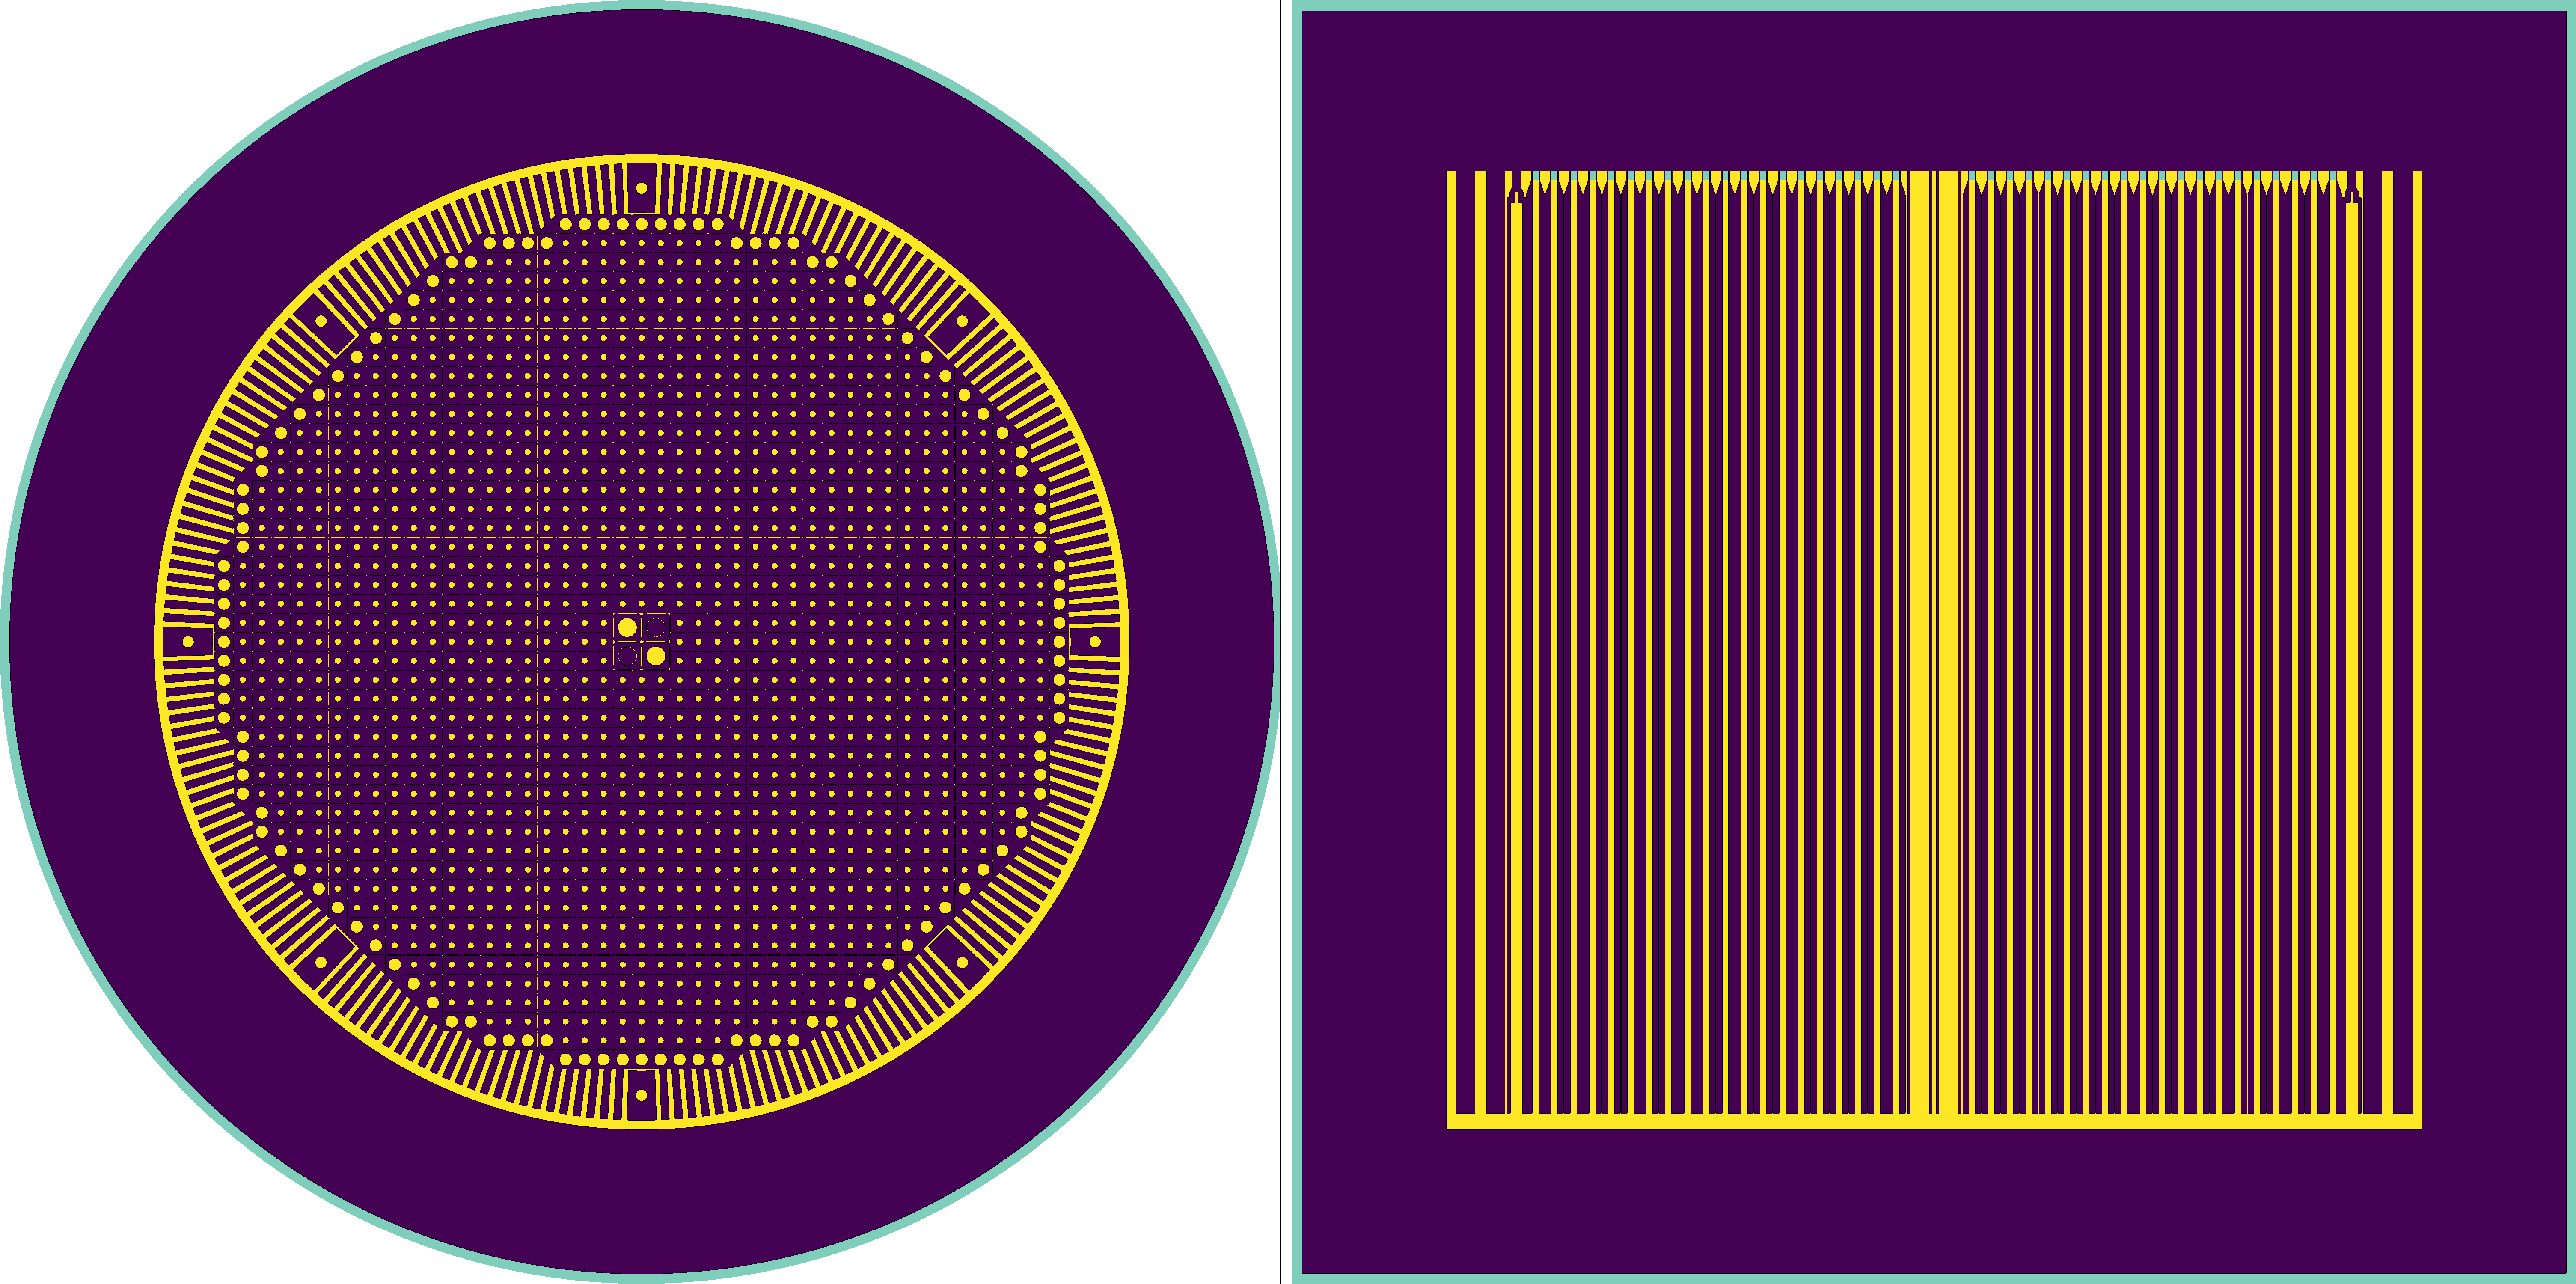
\includegraphics[width=\textwidth]{view_serpent.png}
  \caption{Plan and elevation views of SERPENT 2 \gls{MSBR} model developed in 
  this work.}
  \label{fig:serpent_plan_view}
\end{figure}

\begin{figure}[t!] % replace 't' with 'b' to \centering
  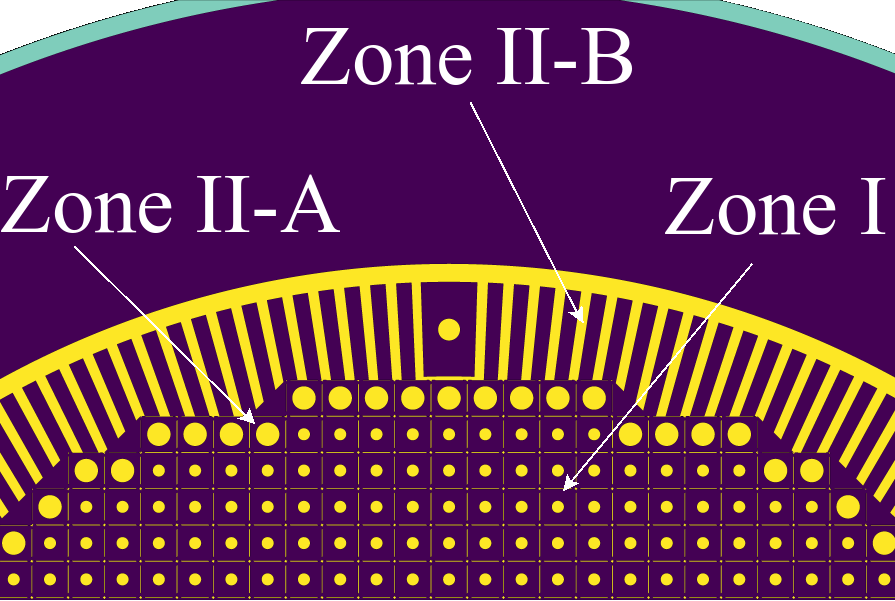
\includegraphics[width=\textwidth]{ser_zone_II.png}
  \caption{Detailed view of \gls{MSBR} two zone model. 
          Yellow represents fuel salt, purple represents graphite, and aqua represents the reactor vessel.}
  \label{fig:serpent_zoneII}
\end{figure}

Since reactor graphite experiences significant dimensional changes due to 
neutron irradiation, the reactor core was designed for periodic replacement. 
Based on the experimental irradiation data from the \gls{MSRE}, the core graphite 
lifetime is about 4 years and the reflector graphite lifetime is 30 years 
\cite{robertson_conceptual_1971}.

There are eight symmetric graphite slabs with a width of 15.24 cm in zone II, 
one of which is illustrated in Figure~\ref{fig:serpent_zoneII}. The holes in 
the centers are for the core lifting rods used during the core replacement 
operations. These holes also allow a portion of the fuel salt to flow to the 
top of the vessel for cooling the top head and axial reflector. 
Figure~\ref{fig:serpent_zoneII} also shows
the 5.08-cm-wide annular 
space between the removable core graphite in zone II-B and the permanently 
mounted reflector graphite. This annulus consists entirely of fuel salt, 
provides space for moving the core assembly, helps compensate for the elliptical 
dimensions of the reactor vessel, and serves to reduce the damaging flux at the 
surface of the graphite reflector blocks. 

$^{135}$Xe is a strong neutron poison, and some fraction of this gas 
is absorbed by graphite during \gls{MSBR} operation. ORNL calculations show 
that for unsealed commercial graphite with helium permeability 10$^{-5}$ 
cm$^2$/s the calculated poison fraction is less than 2\% 
\cite{robertson_conceptual_1971}.  This parameter can be improved by using 
experimental graphites or by applying sealing technology. The effect of the 
gradual poisoning of the core graphite with xenon is not treated here.

\subsubsection{Core zone I}
The central region of the core, called zone I, is made up of graphite elements, 
each $10.16$cm$\times$10.16cm$\times$396.24cm. Zone I has 4 channels for 
control rods: two for graphite rods which both regulate and shim during normal 
operation, and two for backup safety rods consisting of boron carbide clad to 
assure sufficient negative reactivity for emergency situations.

These graphite elements have a mostly rectangular shape with lengthwise ridges 
at each corner that leave space for salt flow elements. Various element sizes 
reduce the peak damage flux and power density in the center of the core to 
prevent local graphite damage.  Figure~\ref{fig:I_element_ref} shows the 
elevation and plan views of graphite elements of zone I 
\cite{robertson_conceptual_1971} and their SERPENT model 
\cite{rykhlevskii_full-core_2017}.

\begin{figure}[ht!] % replace 't' with 'b' to \centering
  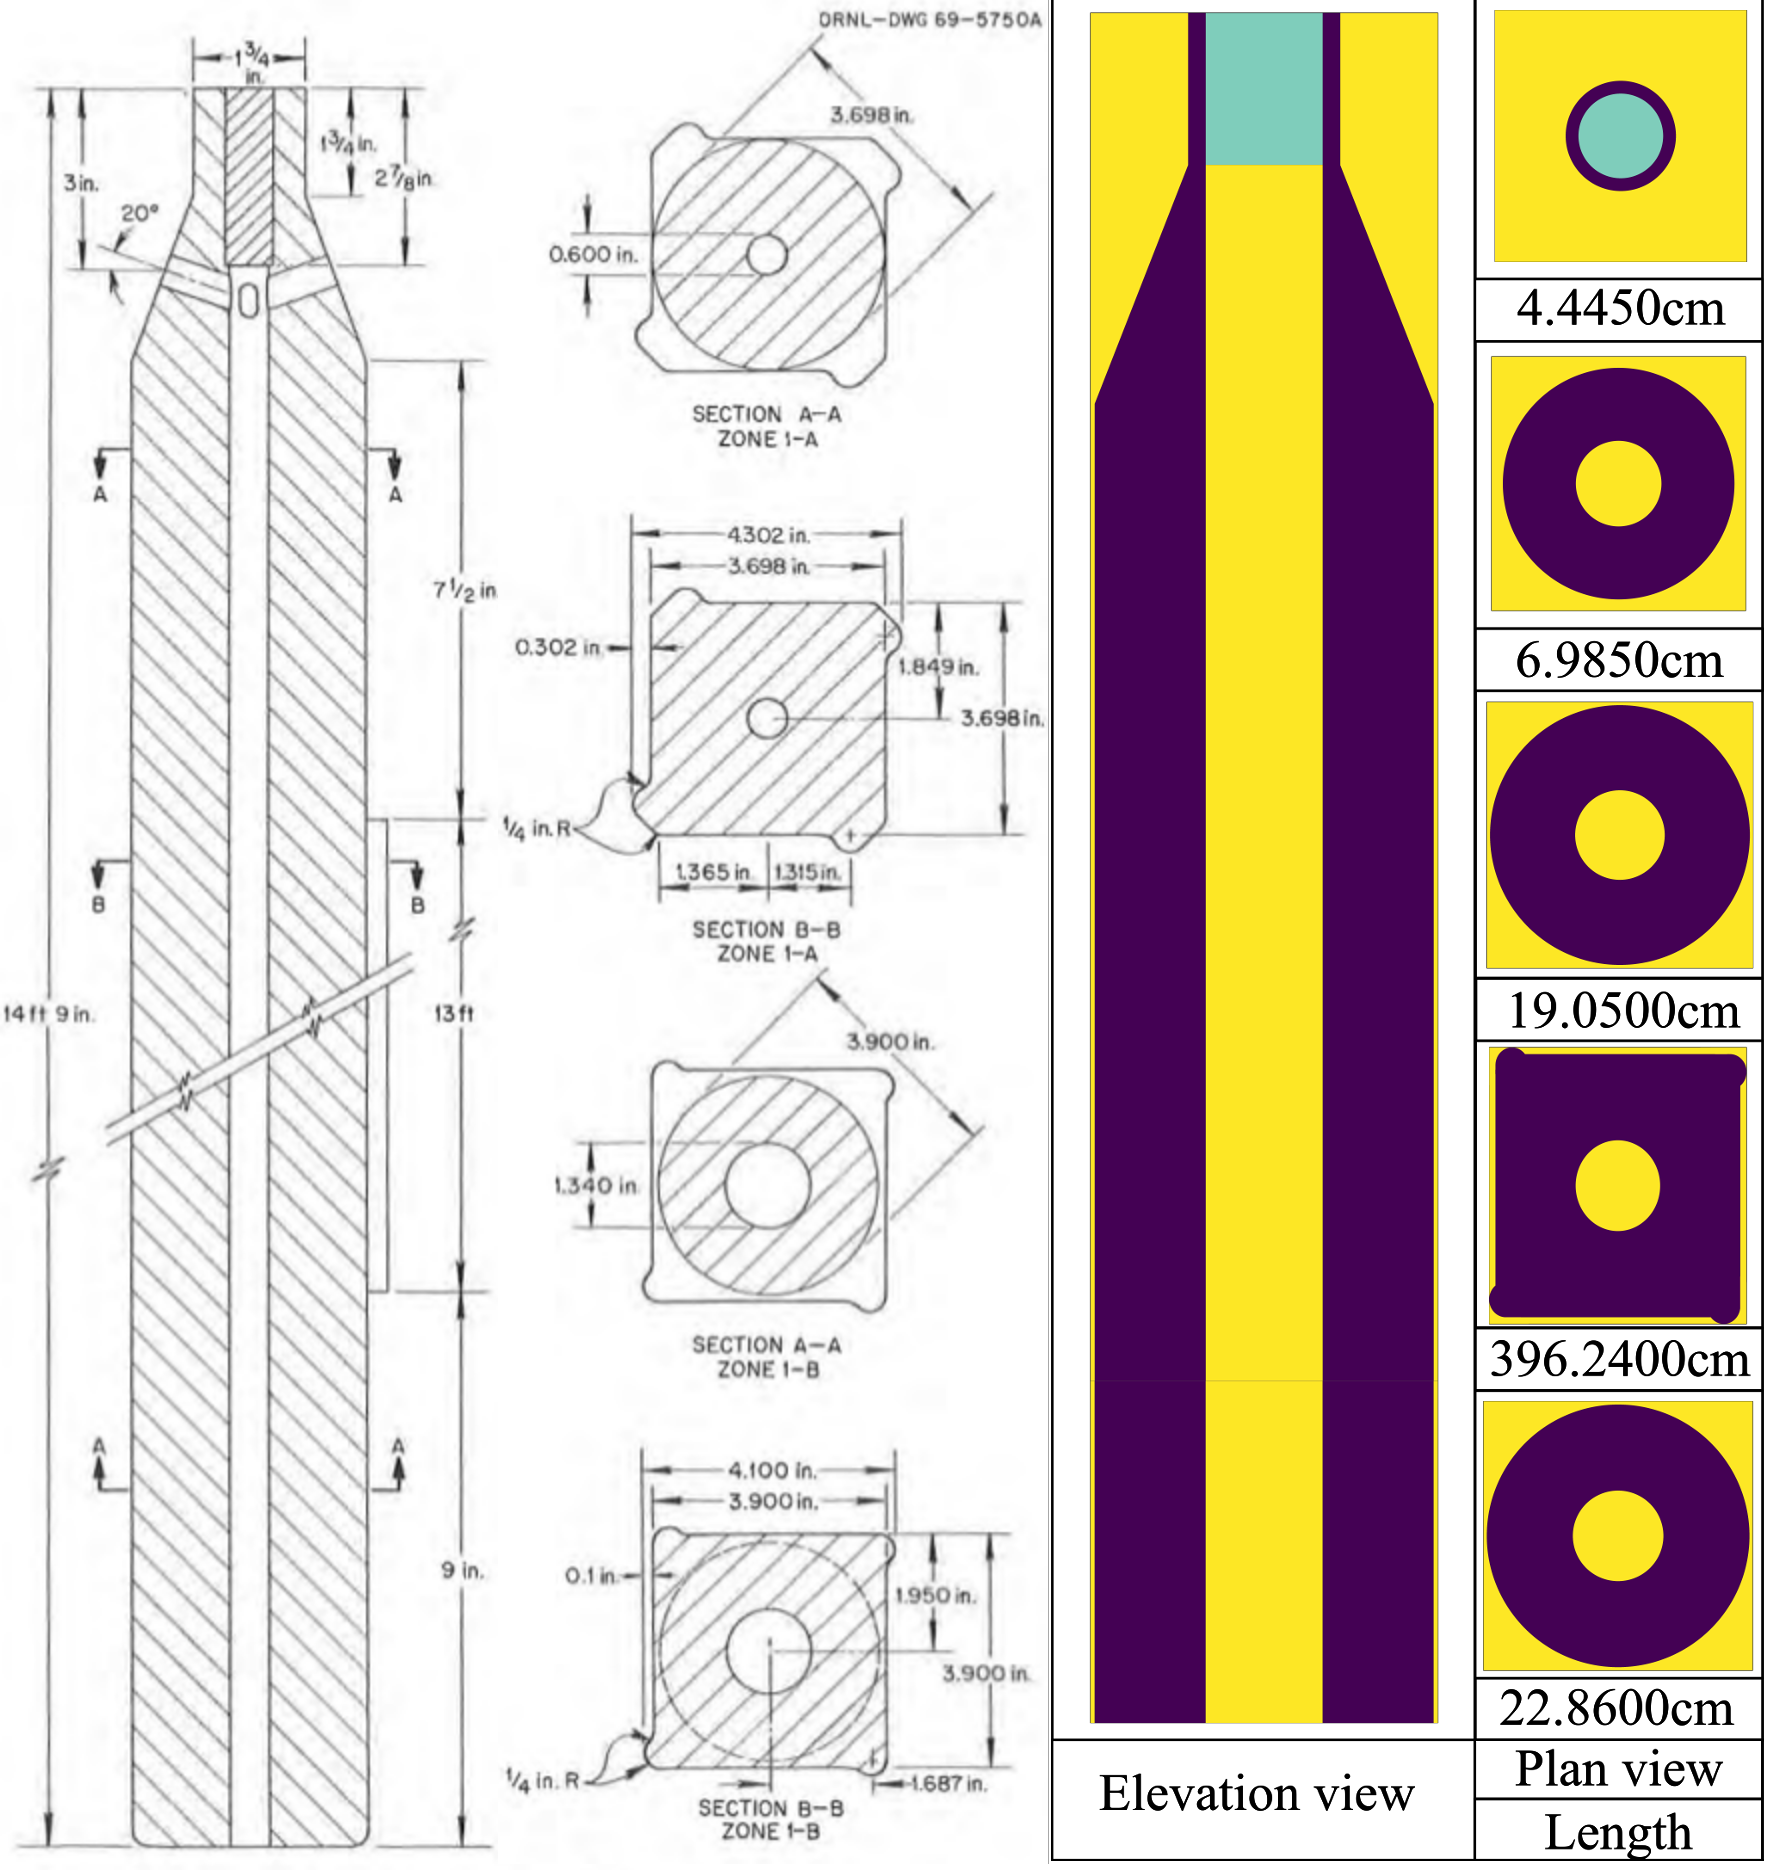
\includegraphics[width=\textwidth]{zone_I_element_ref.png}
  \caption{Graphite moderator elements for zone I 
  \cite{robertson_conceptual_1971,rykhlevskii_full-core_2017}.  Yellow 
  represents fuel salt, purple represents graphite, and aqua represents the 
  reactor vessel.}
  \label{fig:I_element_ref}
\end{figure}

\subsubsection{Core zone II}
Zone II, which is undermoderated, surrounds zone I. Combined with the bounding 
radial reflector, zone II serves to diminish neutron leakage. Two kinds of 
elements form this zone: large-diameter fuel channels (zone II-A) and 
radial graphite slats (zone II-B). 

Zone II has 37\% fuel salt by volume and each element has a fuel channel 
diameter of 6.604cm. The graphite elements for zone II-A are prismatic with
elliptical dowels running axially between the prisms. These dowels
isolate the fuel salt flow in zone I from that in zone II. 
Figure~\ref{fig:II_element_ref} shows the shapes and dimensions of these graphite 
elements and their SERPENT model. Zone II-B elements are rectangular slats 
spaced far enough apart to provide the 0.37 fuel salt volume fraction. The 
reactor zone II-B graphite 5.08cm-thick slats vary in the radial dimension 
(average width is 26.67cm) as shown in figure~\ref{fig:serpent_zoneII}. Zone II 
serves as a blanket to achieve the best performance: a high breeding ratio and 
a low fissile inventory. The harder neutron energy spectrum in zone II 
enhances the rate of thorium resonance capture relative to the fission rate, 
thus limiting the neutron flux in the outer core zone and reducing the neutron 
leakage \cite{robertson_conceptual_1971}. 

The sophisticated, irregular shapes of the fuel elements challenge an accurate 
representation of zone II-B.  
The suggested design \cite{robertson_conceptual_1971} of zone II-B has 8 
irregularly-shaped graphite elements as well as dozens of salt channels. 
These graphite elements were simplified into right-circular cylindrical shapes  
with central channels. Figure~\ref{fig:serpent_zoneII} illustrates this core 
region in the SERPENT model. The volume of fuel salt in zone II was kept 
exactly at 37\%, so that this simplification did not considerably change the core 
neutronics. Simplyfying the eight edge channels was the only simplification made 
to the \gls{MSBR} geometry in this work. 

\begin{figure}[ht!] % replace 't' with 'b' to \centering
  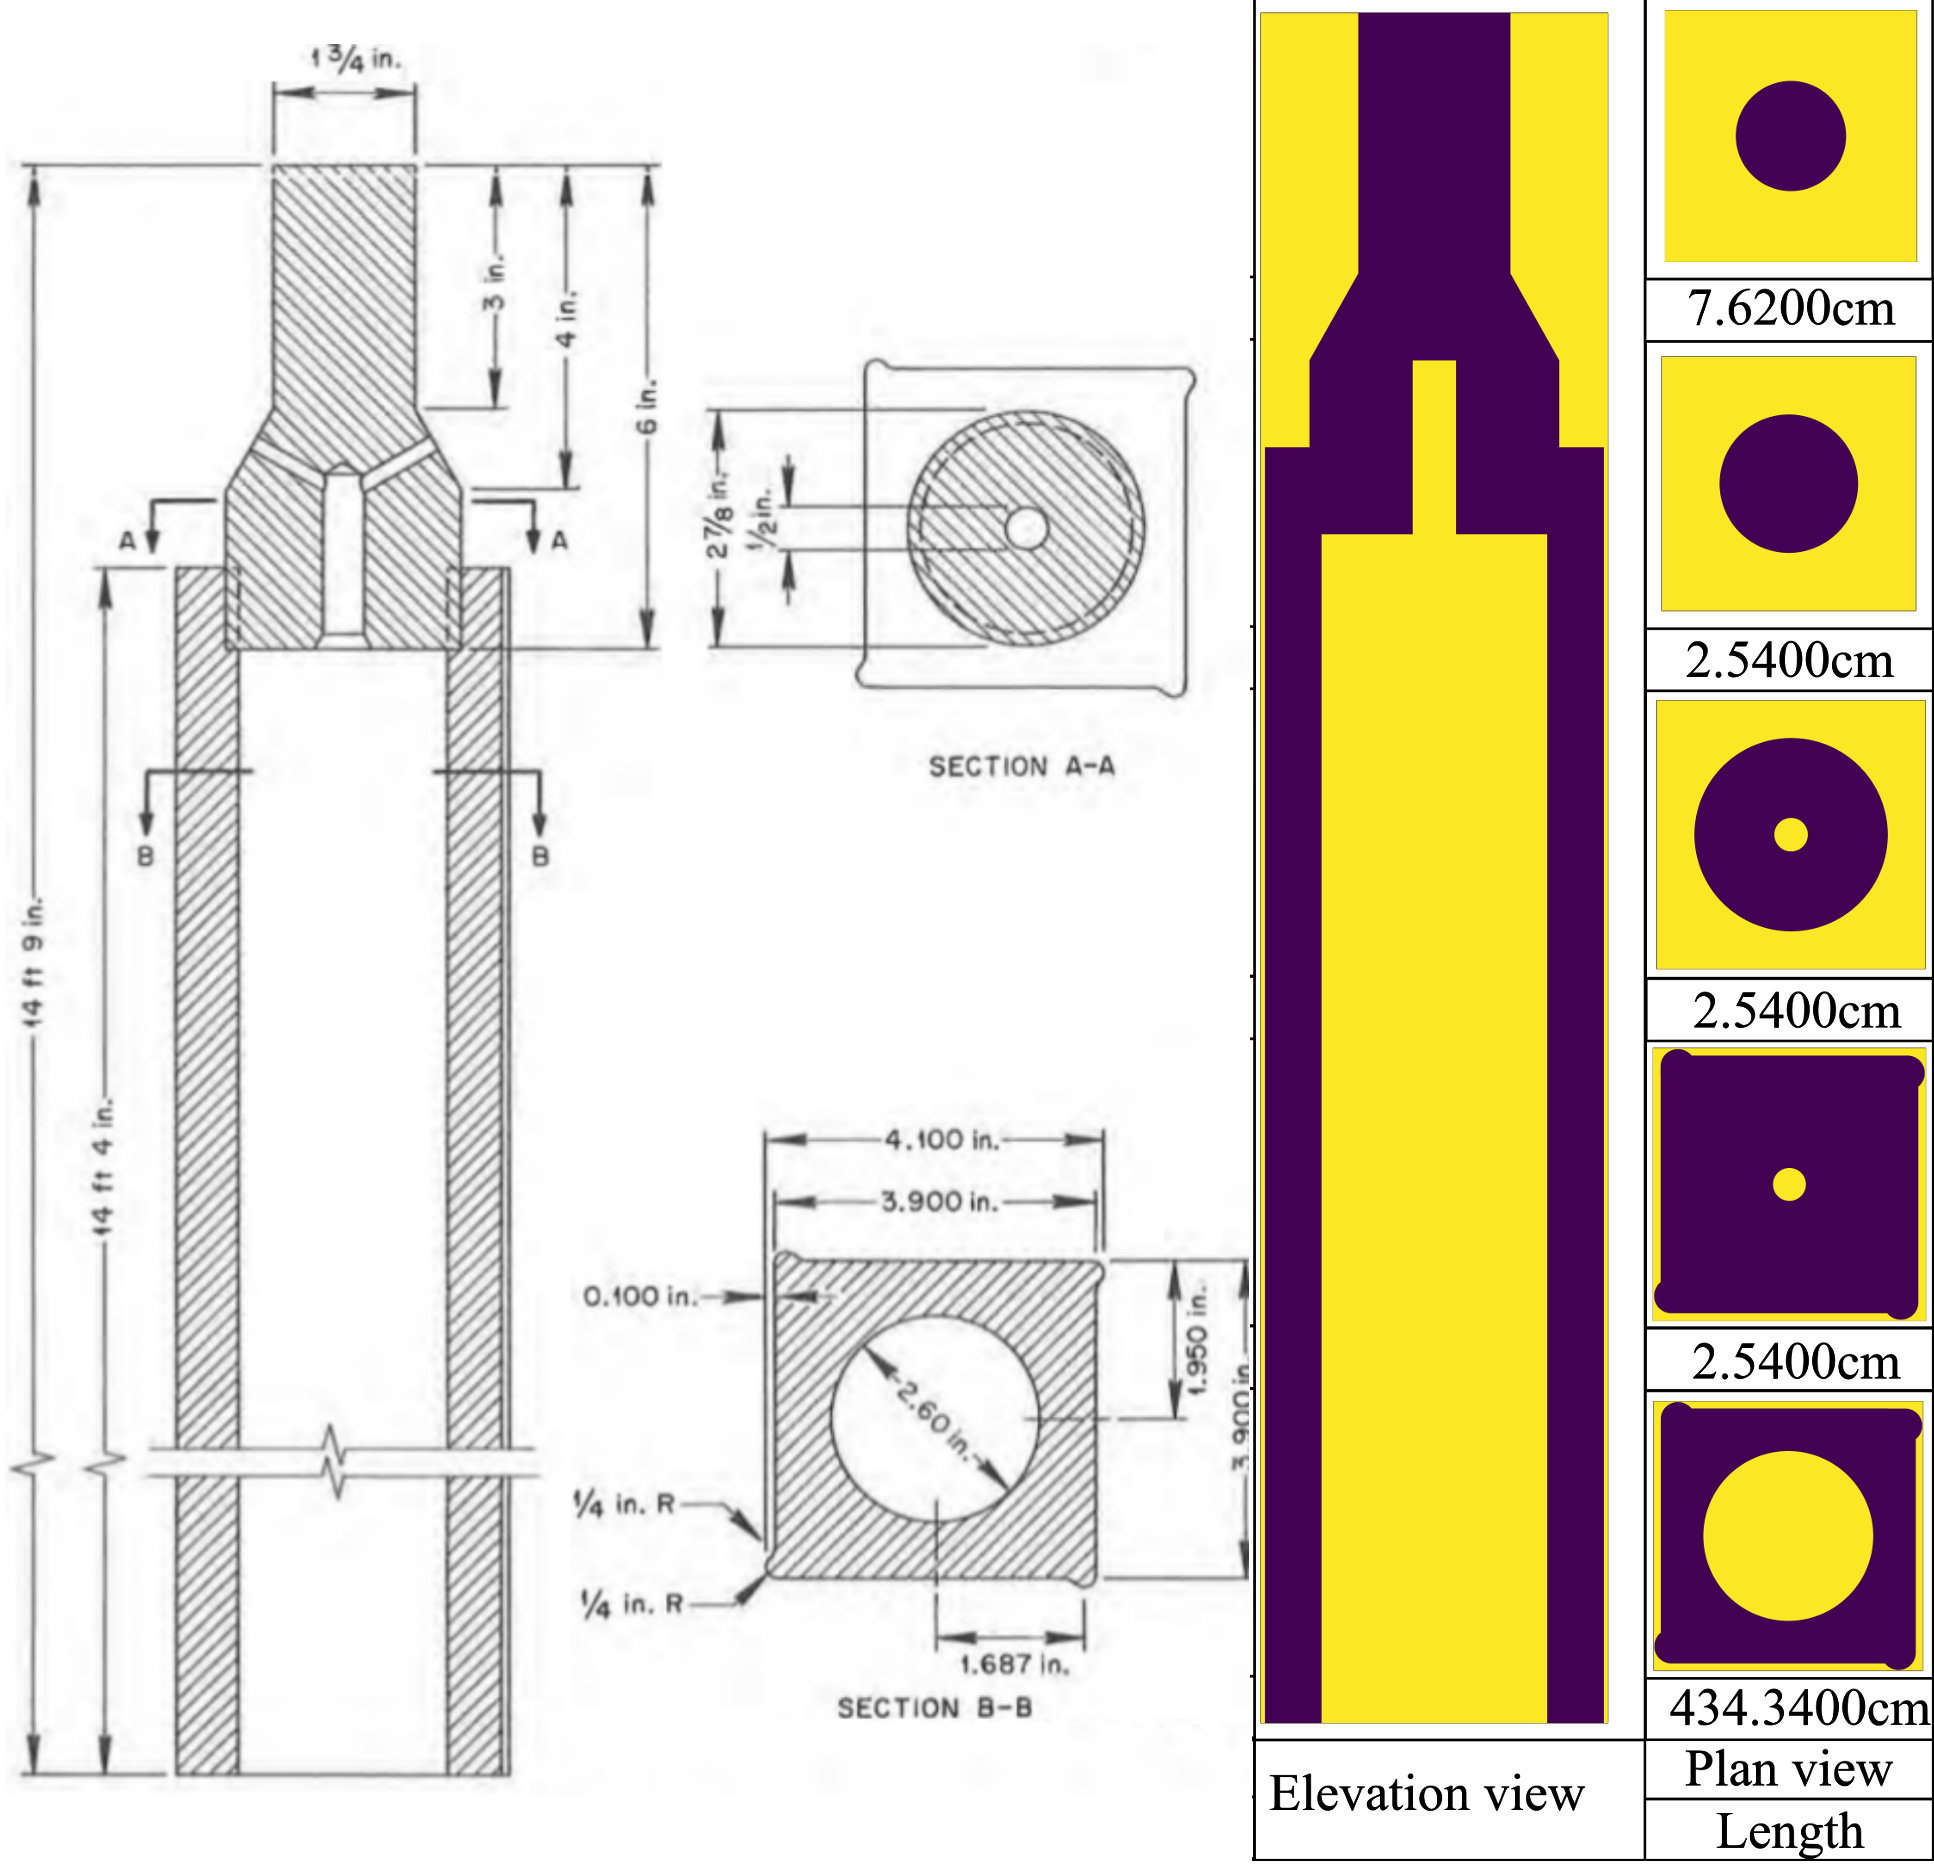
\includegraphics[width=\textwidth]{zone_II_element_ref.png}
  \caption{Graphite moderator elements for zone II-A 
  \cite{robertson_conceptual_1971,rykhlevskii_full-core_2017}.  Yellow 
  represents fuel salt and purple represents graphite.}
  \label{fig:II_element_ref}
\end{figure}

\subsubsection{Material composition and normalization parameters}
The fuel salt, reactor graphite, and modified Hastelloy-N
are all materials created at \gls{ORNL} specifically for the \gls{MSBR}.
The initial fuel salt used the same 
density (3.35 g/cm$^3$) and composition LiF-BeF$_2$-ThF$_4$-$^{233}$UF$_4$ 
(71.75-16-12-0.25 mole \%) as the \gls{MSBR} design 
\cite{robertson_conceptual_1971}. The lithium in the molten salt fuel is fully 
enriched to 100\% $^{7}$Li because $^{6}$Li is a very strong neutron poison and 
becomes tritium upon neutron capture. 

The JEFF-3.1.2 neutron library provided cross section generation 
\cite{oecd/nea_data_bank_jeff-3.1.2_2014}. 
The specific temperature was fixed for each material and did not change during 
the reactor operation. The isotopic 
composition of each material at the initial state was described in detail in 
the MSBR conceptual design study \cite{robertson_conceptual_1971} and has been 
applied to the SERPENT model without any modification. Table~\ref{tab:msbr_tab} is 
a summary of the major \gls{MSBR} parameters used by this model 
\cite{robertson_conceptual_1971}. 

%%%%%%%%%%%%%%%%%%%%%%%%%%%%%%%%%%%%%%%%
\begin{table}[h!]
        \caption{Summary of principal data for \gls{MSBR} 
        \cite{robertson_conceptual_1971}.}
        \begin{tabularx}{\textwidth}{ s  s}
        \hline
                Thermal capacity of reactor           		& 2250 MW(t)
                \\ Net electrical output                 		& 1000 
        MW(e) \\  Net thermal efficiency        				
        & 44.4\%
                \\  Salt volume fraction in central zone I		& 0.13
                \\ Salt volume fraction in outer zone II       & 0.37
                \\ Fuel salt inventory (Zone I)                & 8.2 m$^3$	
        \\ Fuel salt inventory (Zone II)               & 10.8 m$^3$	\\ Fuel 
        salt inventory (annulus)               & 3.8 m$^3$	\\  Total fuel 
        salt inventory                   & 48.7 m$^3$	\\ Fissile mass in fuel 
        salt                   & 1303.7 kg	\\ Fuel salt components                  
                               & LiF-BeF$_2$-ThF$_4$-$^{233}$UF$_4$	\\  
        Fuel salt composition                 & 71.75-16-12-0.25 mole\%
                \\
                Fuel salt density                    & 3.35 g/cm$^3$
                \\ \hline
        \end{tabularx}
        \label{tab:msbr_tab}
\end{table}
%%%%%%%%%%%%%%%%%%%%%%%%%%%%%%%%%%%%%%%%%%%%%%%%

\subsection{Online reprocessing method}
Removing specific chemical elements from a molten salt 
requires intelligent design (e.g., chemical separations equipment design, 
fuel salt flows to equipment) and has a considerable economic cost. All 
liquid-fueled \gls{MSR} designs involve varying levels of online fuel 
processing. Minimally, volatile gaseous fission products (e.g. Kr, Xe) escape 
from the fuel salt during routine reactor operation and must be captured. 
Additional systems might be used to enhance removal of those elements. Most 
designs also call for the removal of noble and rare earth metals from the core 
since these metals act as neutron poisons. Some designs suggest a more complex 
list of elements to process (figure~\ref{fig:periodic_tab}), including the 
temporary removal of protactinium or other regulation of the 
actinide inventory \cite{ahmad_neutronics_2015}.

\begin{figure}[htp!] % replace 't' with 'b' to \centering
  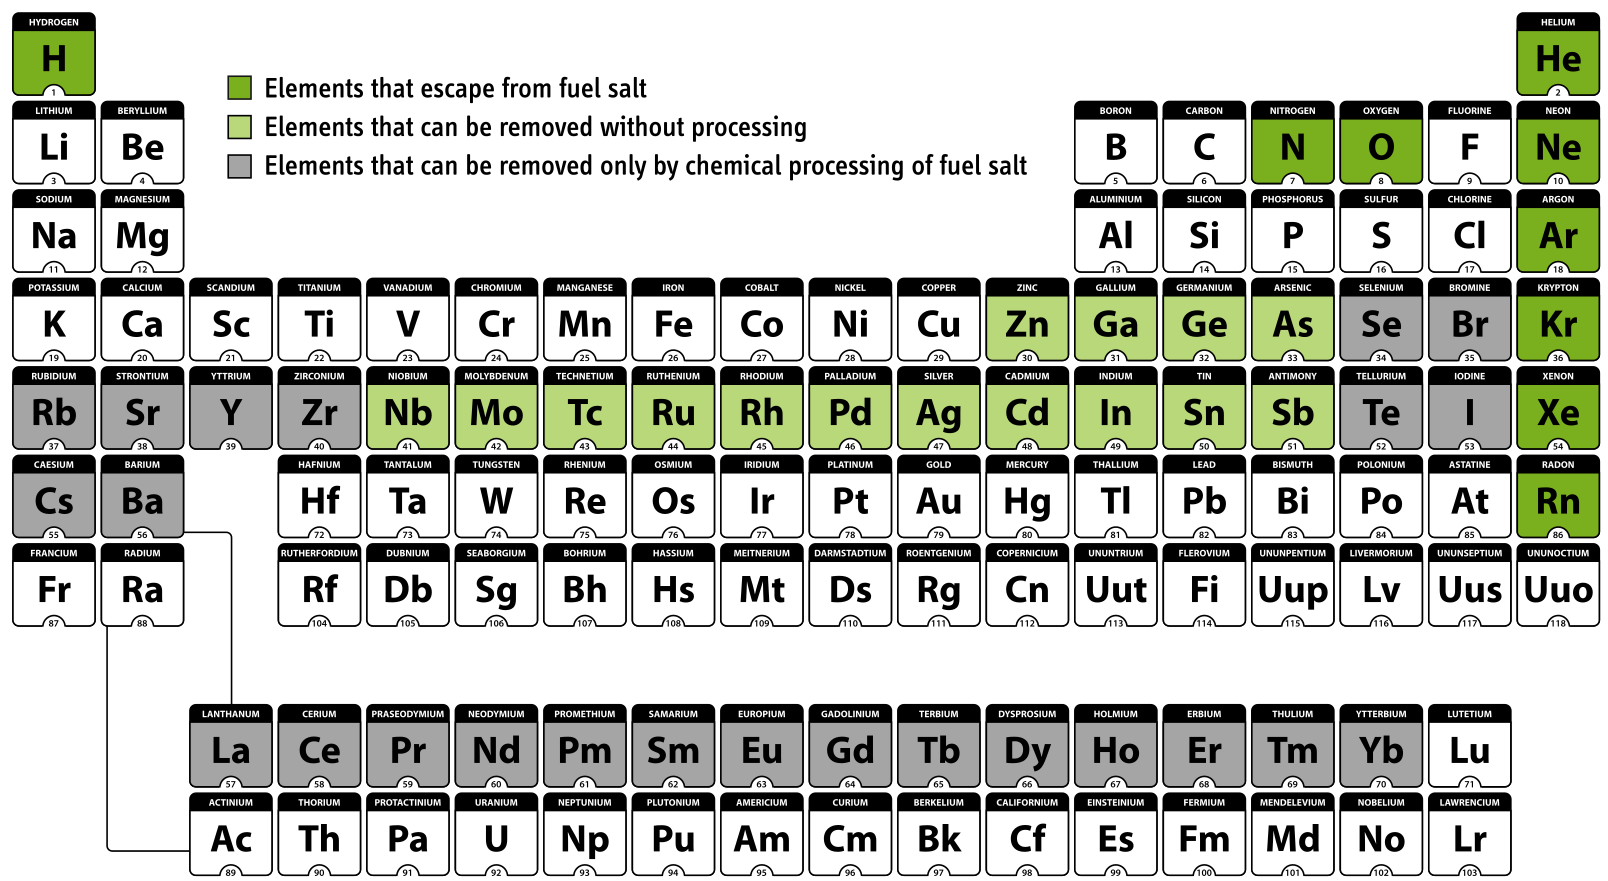
\includegraphics[width=\textwidth]{periodic_map.png}
  \caption{Processing options for \gls{MSR} fuels. 
          Reproduced from \cite{ahmad_neutronics_2015} where it was adapted 
          from a chart courtesy of Nicolas 
          Raymond, www.freestock.ca.}
  \label{fig:periodic_tab}
\end{figure}

\subsubsection{Fuel material flows}
The $^{232}$Th in the fuel absorbs thermal neutrons and produces $^{233}$Pa 
which then decays into the fissile $^{233}$U. Furthermore, the \gls{MSBR} 
design requires online reprocessing to remove all poisons (e.g. $^{135}$Xe), 
noble metals, and gases (e.g. $^{75}$Se, $^{85}$Kr) every 20 seconds. 
Protactinium presents a challenge, since it has a large absorption cross 
section in the thermal energy spectrum. Moreover, $^{233}$Pa left in the core
would produce $^{234}$Pa and $^{234}$U, neither of which are useful as fuel. 
Accordingly, $^{233}$Pa is continuously 
removed from the fuel salt into a protactinium decay tank to allow $^{233}$Pa 
to decay to $^{233}$U without the corresponding negative neutronic impact. The reactor 
reprocessing system must separate $^{233}$Pa from the molten-salt fuel over 3 
days, hold it while $^{233}$Pa decays into $^{233}$U, and return it back to the 
primary loop. This feature allows the reactor to avoid neutron losses to 
protactinium, lowers in-core fission product inventory, and increases the 
efficiency of $^{233}$U breeding. Table~\ref{tab:reprocessing_list} summarizes 
full list of nuclides and the ``cycle times''\footnote{ The \gls{MSBR} program defined a ``cycle time" as the amount of time required to remove 100\% of a target nuclide from a fuel 
salt \cite{robertson_conceptual_1971}.} used for modeling salt treatment and 
separations \cite{robertson_conceptual_1971}. 

%%%%%%%%%%%%%%%%%%%%%%%%%%%%%%%%%%%%%%%%
\begin{table}[ht!]
        \caption{The effective cycle times for protactinium and fission 
        products removal (reproduced from \cite{robertson_conceptual_1971}).}
        \begin{tabularx}{\textwidth}{ x | s | x }
        \hline Processing group & \qquad\qquad\qquad Nuclides & Cycle time (at 
                full power) \\ \hline Rare earths & Y, La, Ce, Pr, Nd, Pm, Sm, 
                Gd & 50 days \\ \qquad & Eu & 500 days \\ Noble metals & Se, 
                Nb, Mo, Tc, Ru, Rh, Pd, Ag, Sb, Te & 20 sec \\
        Seminoble metals & Zr, Cd, In, Sn & 200 days \\
        Gases & Kr, Xe & 20 sec \\ Volatile fluorides & Br, I & 60 days \\
        Discard & Rb, Sr, Cs, Ba & 3435 days \\ 
        %Salt discard & Th, Li, Be, F & 3435 days \\ 
        Protactinium & $^{233}$Pa & 3 days \\ Higher 
                nuclides & $^{237}$Np, $^{242}$Pu & 16 years \\  \hline
        \end{tabularx}
        \label{tab:reprocessing_list}
\end{table}
The removal rates vary among nuclides in this reactor concept which dictate the 
necessary resolution of depletion calculations. If the depletion time intervals 
are very short, an enormous number of depletion steps are required to obtain 
the equilibrium composition. On the other hand, if the depletion  calculation 
time interval is too long, the impact of short-lived fission products is not 
captured. To compromise, a 3 day time interval was selected for depletion 
calculations\footnote{ Optimal depletion time step of 3 days for \gls{MSR} 
batch-wise depletion simulation was first described and concluded by Powers 
\emph{et al.} \cite{powers_new_2013}.} to correlate with the removal interval 
of 
$^{233}$Pa and $^{232}$Th was continuously added to maintain the initial mass 
fraction of $^{232}$Th.

\subsubsection{The SaltProc modeling and simulation code}
The SaltProc tool \cite{rykhlevskii_arfc/saltproc:_2018} is designed to 
expand SERPENT 2
 depletion capabilities for modeling liquid-fueled \gls{MSR} for continuous 
 reprocessing.
The Python package uses HDF5 \cite{the_hdf_group_hierarchical_1997} to store 
data, and the PyNE Nuclear Engineering Toolkit \cite{scopatz_pyne:_2012}
for SEPRENT output file parsing and nuclide naming. SaltProc is an open-source tool 
that uses a semi-continuous approach to simulate continuous feeds and removals 
in \glspl{MSR}. 

The tool structure and capabilities of SaltProc are similar to the ChemTriton tool 
developed in \gls{ORNL} for SCALE \cite{powers_new_2013}. SaltProc is coupled 
with the Monte Carlo SERPENT 2
software to simulate online reprocessing for irregular full-core 
geometry with high fidelity.  The primary function of SaltProc is to 
manage material streams while SERPENT 2 performs the neutron 
transport and depletion calculations. Saltproc is defined as a python class, where 
each material stream is defined as a isotopic atomic density
vector variable. This allows tracking of time-sensitive material streams such 
as the 	$^{233}$Pa tank in the \gls{MSBR}. The user can define the reprocessing 
parameters, such as the reprocessing interval and removal efficiency.  In 
addition, SaltProc provides a set of functions for each stream: read and write 
isotopic data in/from database, separate out specific elements from stream with 
defined efficiency, feed in specific isotopes to stream, and maintain constant 
number density of specific nuclide in the core. These attributes and functions 
are crucial to simulating the operation of a complex, multi-zone, multi-fluid 
\gls{MSR} and are sufficiently general to represent myriad reactor systems.

The current version of SaltProc only allows 100\% separation efficiency for 
either specific elements or groups of elements (e.g. Processing Groups as described in 
Table~\ref{tab:reprocessing_list}) at the end of the specific cycle time. 
This simplification neglects the reality that the salt spends appreciable time 
out of the core, in the primary loop pipes and the heat exchanger.  

This approach works well for fast-removing elements (gases, noble metals, 
protactinium) which should be removed each depletion step. Unfortunately, 
for the elements with longer cycle times (i.e. rare earths should be removed 
every 50 days) this simplified approach leads to oscillatory behavior of all
major parameters. In future releases of SaltProc, this drawback will be eliminated 
by removing elements with longer cycle times using different method: only mass 
fraction (calculated separately for each reprocessing group) will be removed each
 depletion step or batch (e.g. 3 days in the current work).

SaltProc, currently in active development on Github (https://github.com/ 
arfc/saltproc), leverages unit tests and continuous integration for 
sustainable development. There is also documentation
generated through Sphinx document generator for ease of use. In future 
releases, we plan to 
implement
support for entirely user-customized reprocessing strategies, two-region \gls{MSR} modeling 
capabilities, and decay modeling in tanks.

Figure~\ref{fig:saltproc_flow} illustrates the  online reprocessing simulation 
algorithm coupling SaltProc and SERPENT 2. To perform a depletion step, 
SaltProc reads a user-defined SERPENT 2 template file. This file contains input 
cards with parameters such as geometry, material, isotopic composition, neutron 
population, criticality cycles, total heating power, and boundary conditions.  
After the depletion calculation, SaltProc reads the depleted fuel composition 
file and stores the depleted composition isotopic vector in 
an HDF5 database. 

SaltProc only stores and edits the isotopic composition of 
the fuel stream, which makes SaltProc a flexible tool to model any geometry: an 
infinite medium, a unit cell, a multi-zone simplified assembly, or a full core.
This flexibiliity allows the user to perform simulations of varying fidelity 
and computational intensity.

\begin{figure}[ht!] % replace 't' with 'b' to \centering
  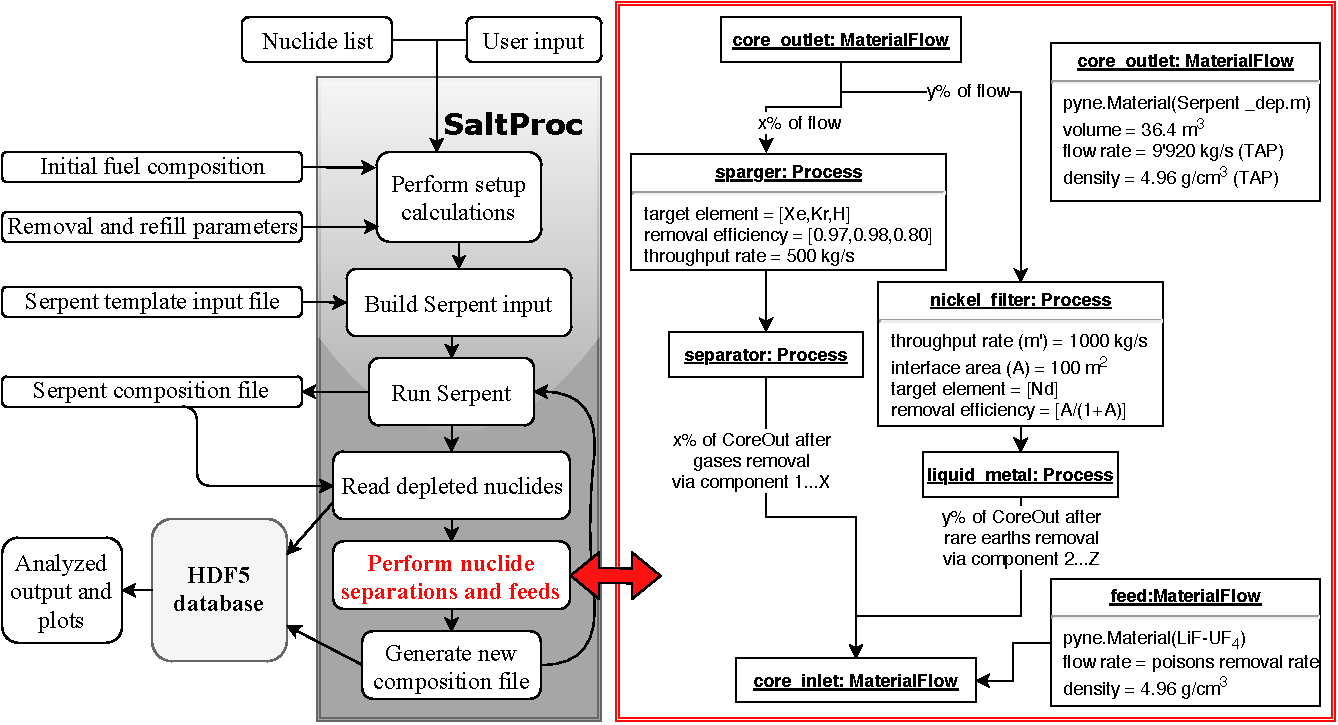
\includegraphics[width=0.75\textwidth]{saltproc_flowchart.pdf}
  \caption{Flow chart for the Saltproc python package.}
  \label{fig:saltproc_flow}
\end{figure}
SaltProc can manage as many material streams as desired. It also may work with 
multiple depletion materials. At the end of each depletion step, SaltProc 
reads the depleted compositions and tracks each material stream individually. 
Following this, it applies chemical separation functions to fuel stream 
vectors. These vectors then form a matrix (isotopics x timesteps) which 
SaltProc stores in an HDF5 database and prints into the SERPENT 2 composition 
file for the next depletion calculation.

SaltProc records every value every timestep. The resulting time series datasets
produced by SaltProc are listed below,
where the values inside the parenthesis are the dataset sizes:

\begin{itemize}
    \item \texttt{core adensity before reproc} (number of isotopes x timesteps)
    \item \texttt{core adensity after reproc} (number of isotopes x timesteps)
    \item \texttt{Keff\_BOC} (1 x timesteps)
    \item \texttt{Keff\_EOC} (1 x timesteps)
    \item \texttt{Th tank adensity} (number of isotopes x timesteps)
    \item \texttt{iso codes} (number of isotopes x 1)
\end{itemize}

In addition, SaltProc is able to define time-dependent material feed and 
removal rates to investigate their impacts. These rates need not be 
constant in SaltProc. They can be defined as piecewise functions or set to 
respond to conditions in the core. For instance, SaltProc might increase the 
fissile material feeding rate if the effective multiplication factor, 
$k_{eff}$, falls below a specific limit (e.g., 1.002).
These capabilities allow SaltProc to analyze fuel cycle of a generic 
liquid-fueled \gls{MSR}. In summary, the development approach of SaltProc 
focused on producing a generic, flexible and expandable tool to give the 
SERPENT 2 Monte Carlo code the ability to conduct advanced in-reactor fuel 
cycle analysis as well as simulate a myriad of online refueling and fuel 
reprocessing systems.

%\FloatBarrier
%\section{Results}
The SaltProc online reprocessing simulation package is demonstrated in four 
applications: (1) analyzing  \gls{MSBR} neutronics and fuel cycle to find the 
equilibrium core composition and core depletion, (2) studying operational and 
safety parameters evolution during \gls{MSBR} operation, (3) demonstrating that 
in a single-fluid two-region \gls{MSBR} conceptual design the undermoderated 
outer core zone II works as a virtual ``blanket'', reduces neutron leakage and 
improves breeding ratio due to neutron energy spectral shift, and (4) 
determining the effect of fission product removal on the core neutronics.

The neutron population per cycle and the number of active/inactive cycles were 
chosen to obtain balance between reasonable uncertainty for a transport problem 
($\leq$ 15 pcm\footnote{ 1 pcm = 10$^{-5}\Delta k_{eff}/k_{eff}$} for effective 
multiplication factor) and computational time. The \gls{MSBR} depletion and 
safety parameter computations were performed on 64 Blue Waters XK7 nodes (two 
AMD 6276 Interlagos CPU per node, 16 floating-point Bulldozer core units per 
node or 32 ``integer'' cores per node, nominal clock speed is 2.45 GHz). The 
total computational time for calculating the equilibrium composition was 
approximately 9,900 node-hours (18 core-years.)

\subsection{Effective multiplication factor}
Figures~\ref{fig:keff}, \ref{fig:keff_zoomed} show the effective multiplication factors 
obtained using SaltProc and SERPENT2. The effective multiplication factors were 
calculated after removing fission products listed in 
Table~\ref{tab:reprocessing_list} and adding the fertile material at the end of 
cycle time (3 days for this work). The effective multiplication 
factor fluctuates significantly as a result of the batch-wise nature of this 
online reprocessing strategy. 

\begin{figure}[ht!] 
  \centering
  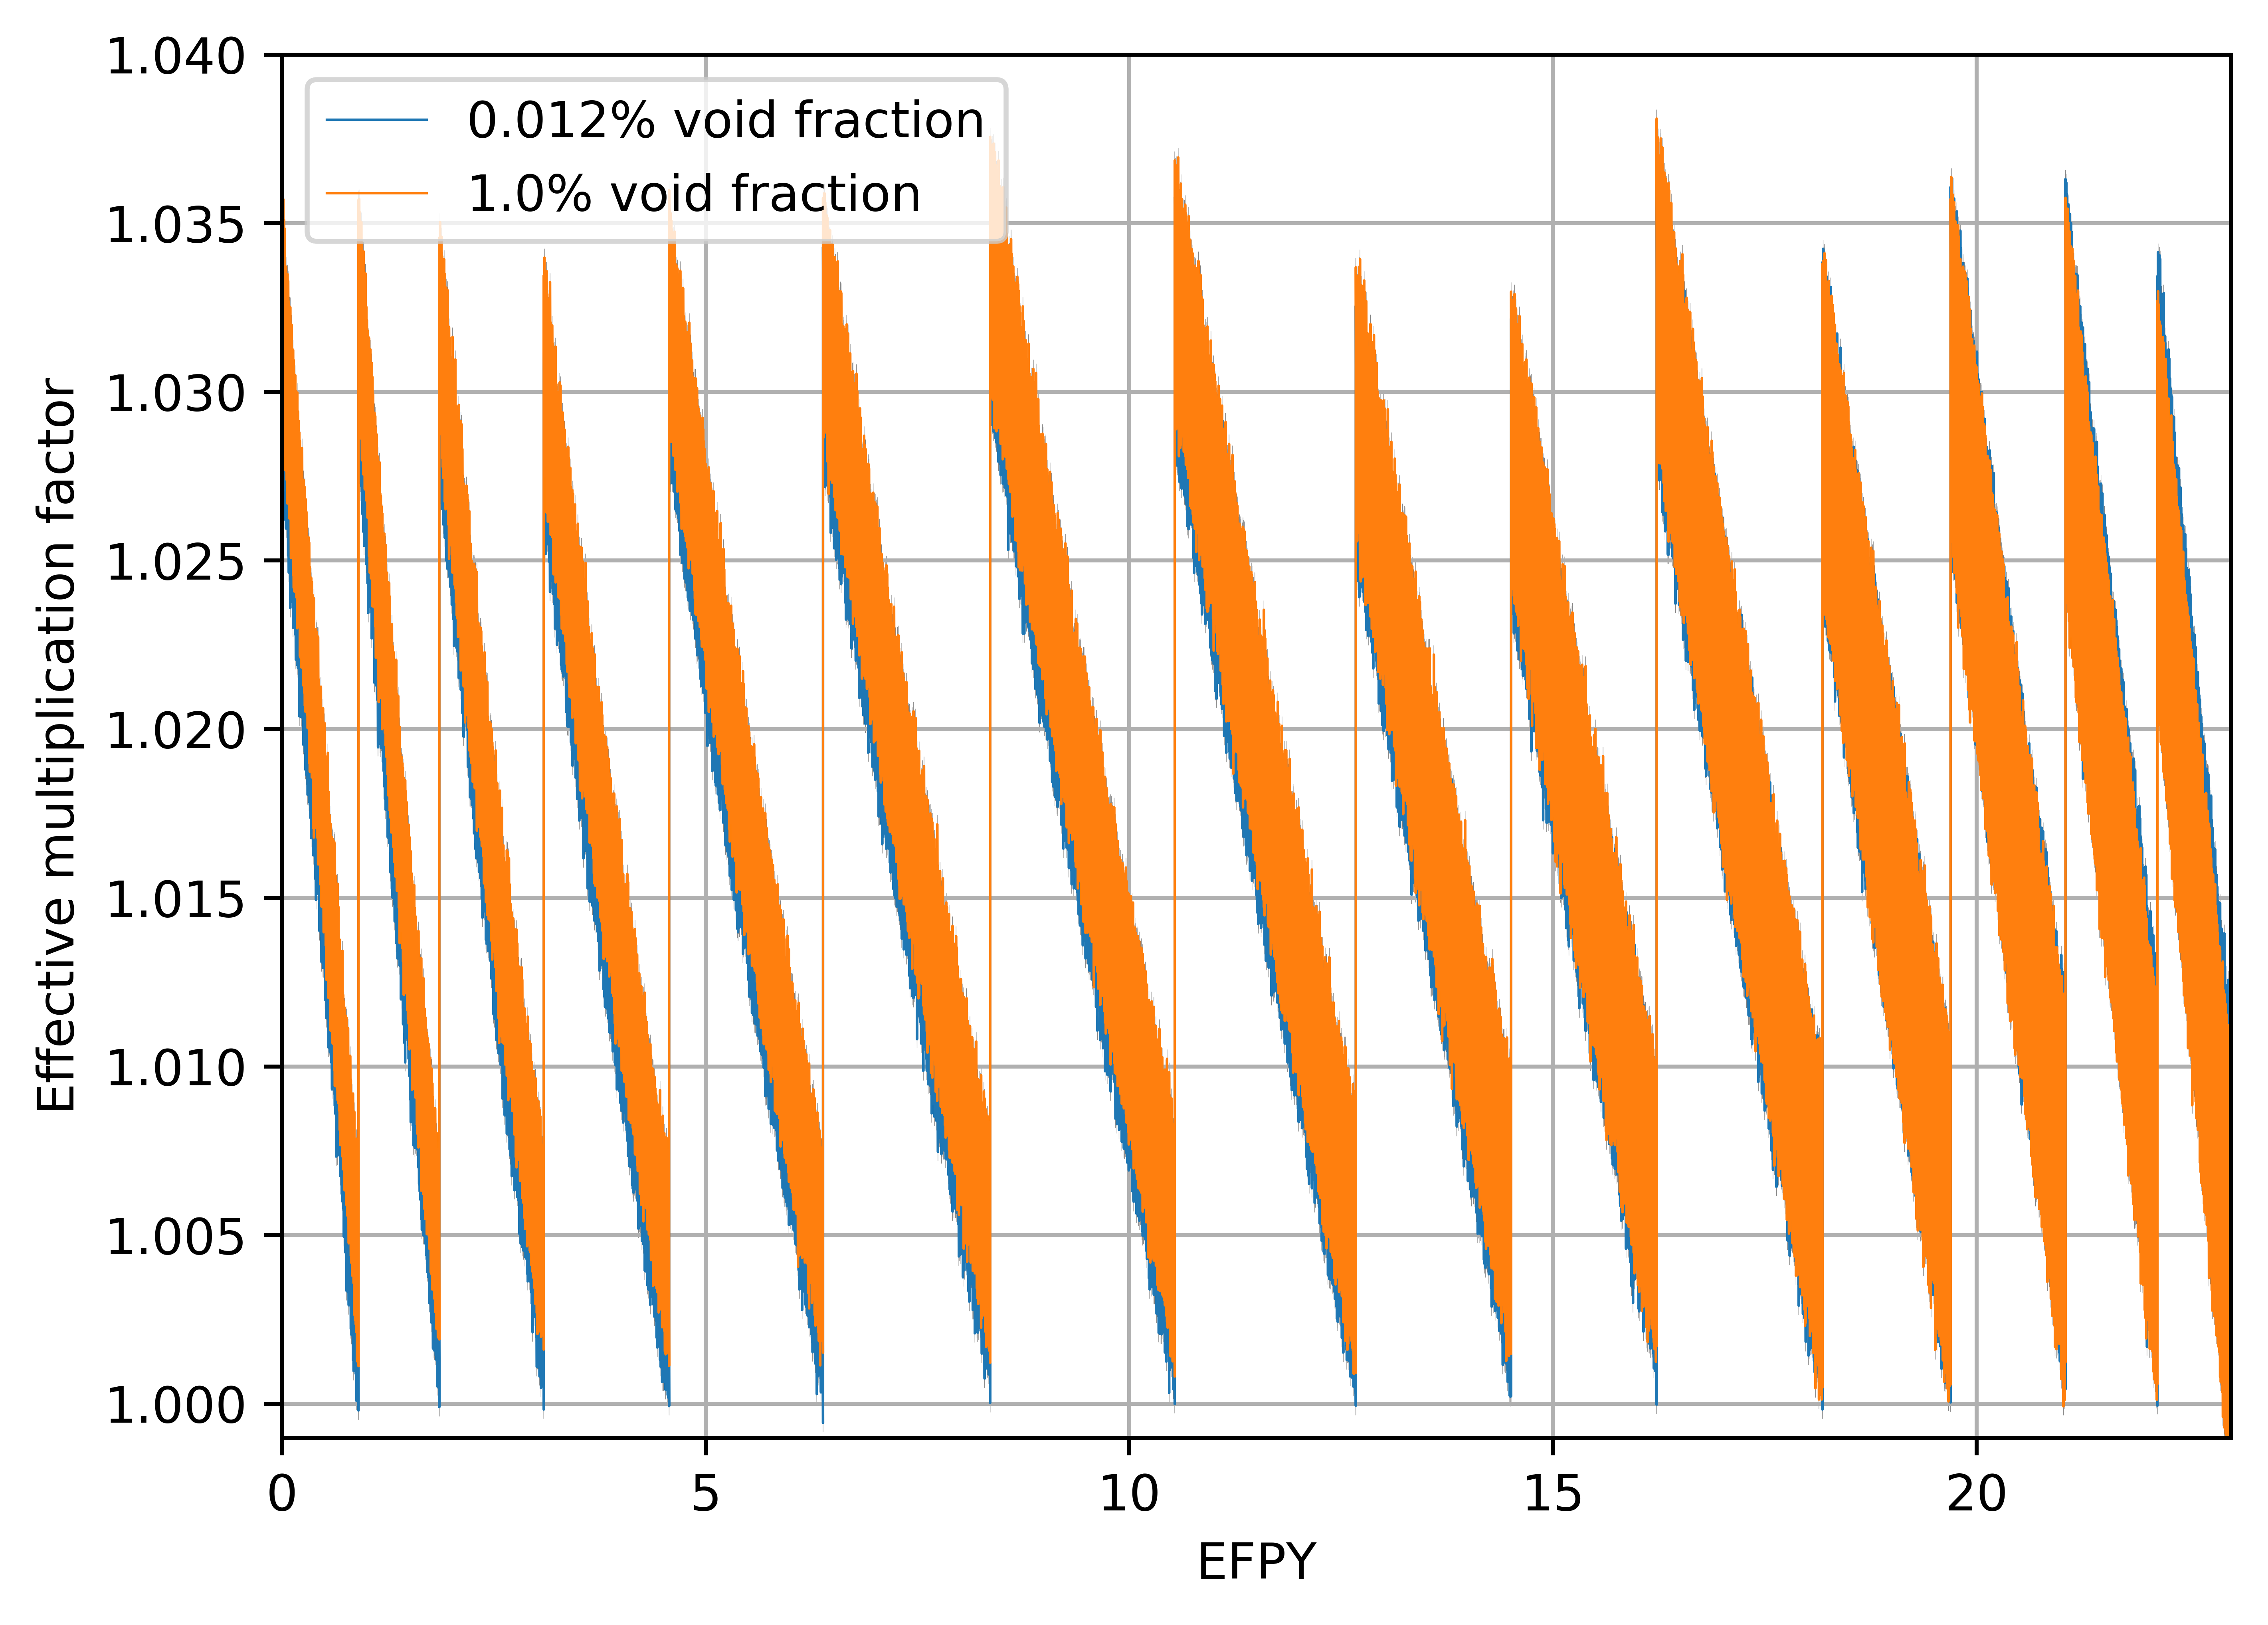
\includegraphics[width=\textwidth]{keff.png}
  \caption{Effective multiplication factor dynamics for full-core \gls{MSBR} 
  model over a 60-year reactor operation lifetime.}
  \label{fig:keff}
\end{figure}
\begin{figure}[ht!] 
  \centering
  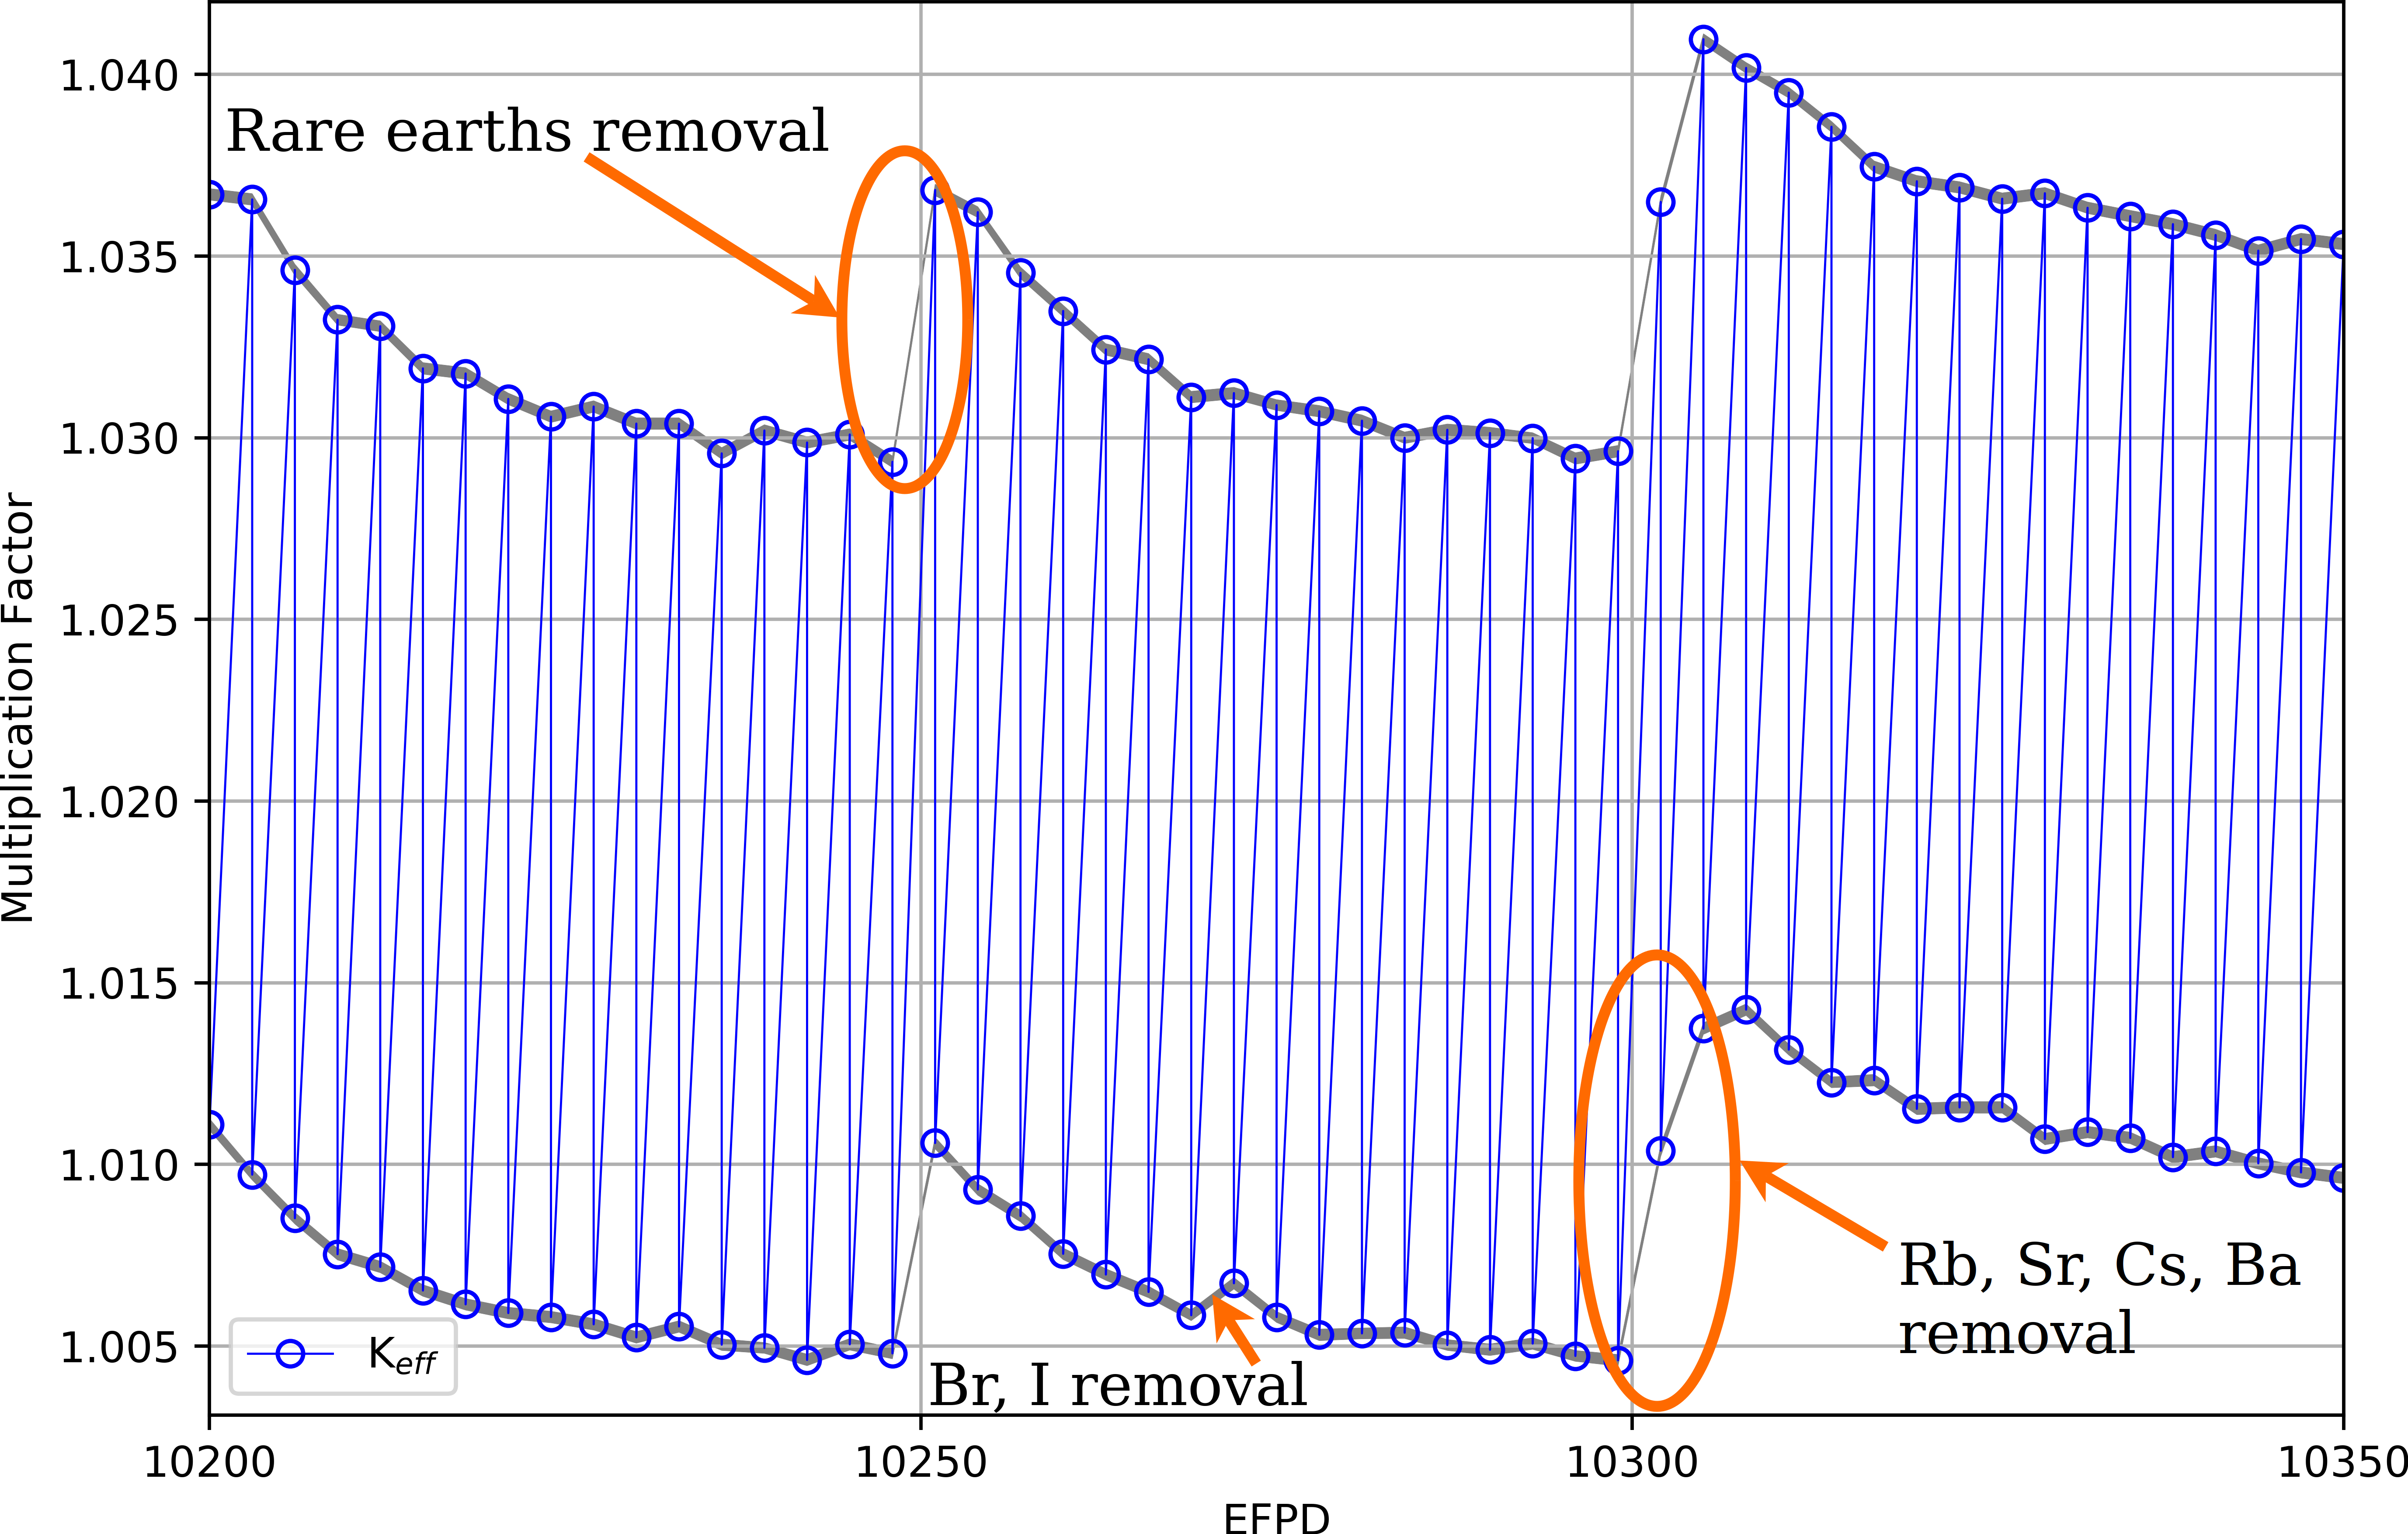
\includegraphics[width=\textwidth]{keff_zoomed.png}
  \caption{Zoomed effective multiplication factor for 150-EFPD time interval.}
  \label{fig:keff_zoomed}
\end{figure}

First, SERPENT calculates the effective multiplication factor for the beginning 
of the cycle (there is fresh fuel composition at the first step). Next, it 
computes the new fuel salt composition at the end of a 3-day depletion. The 
corresponding effective multiplication factor is much smaller than the previous 
one. Finally, SERPENT calculates $k_{eff}$ for the depleted composition after 
applying feeds and removals. The $K_{eff}$ increases accordingly since major reactor 
poisons (e.g. Xe, Kr) are removed, while fresh fissile material ($^{233}$U) 
from the protactinium decay tank is added.  

Additionally, the presence of rubidium, strontium, cesium, and barium in the 
core are disadvantageous to reactor physics. 
Overall, the effective multiplication factor gradually decreases from 1.075 to 
$\approx$1.02 at equilibrium after approximately 6 years of irradiation. 

In fact, SaltProc fully removes 
all of these elements every 3435 days (not a small mass fraction every 3 days) 
which causes the multiplication factor to jump by approximately 450 
pcm, and limits using the batch approach for online reprocessing simulations. 
In future versions of SaltProc this drawback will be eliminated by removing 
elements with longer residence times (seminoble metals, volatile fluorides, Rb, Sr,
 Cs, Ba, Eu). In that approach, chemistry models will inform separation 
 efficiencies for each reprocessing group and removal will optionally be spread more 
 evenly accross the cycle time.

\subsection{Fuel salt composition dynamics}
The analysis of the fuel salt composition evolution provides more comprehensive 
information about the equilibrium state. Figure~\ref{fig:adens_eq} shows the number 
densities of major nuclides which have a strong influence on the reactor core 
physics. The concentration of $^{233}$U, $^{232}$Th, $^{233}$Pa, and $^{232}$Pa in 
the fuel salt change insignificantly after approximately 2500 days of operation. 
In particular, the $^{233}$U number density fluctuates by less than 0.8\% between
 16 and 20 years of operation. Hence, a quasi-equilibrium state was 
achieved after 16 years of reactor operation.
\begin{figure}[ht!] % replace 't' with 'b' to 
  \centering
  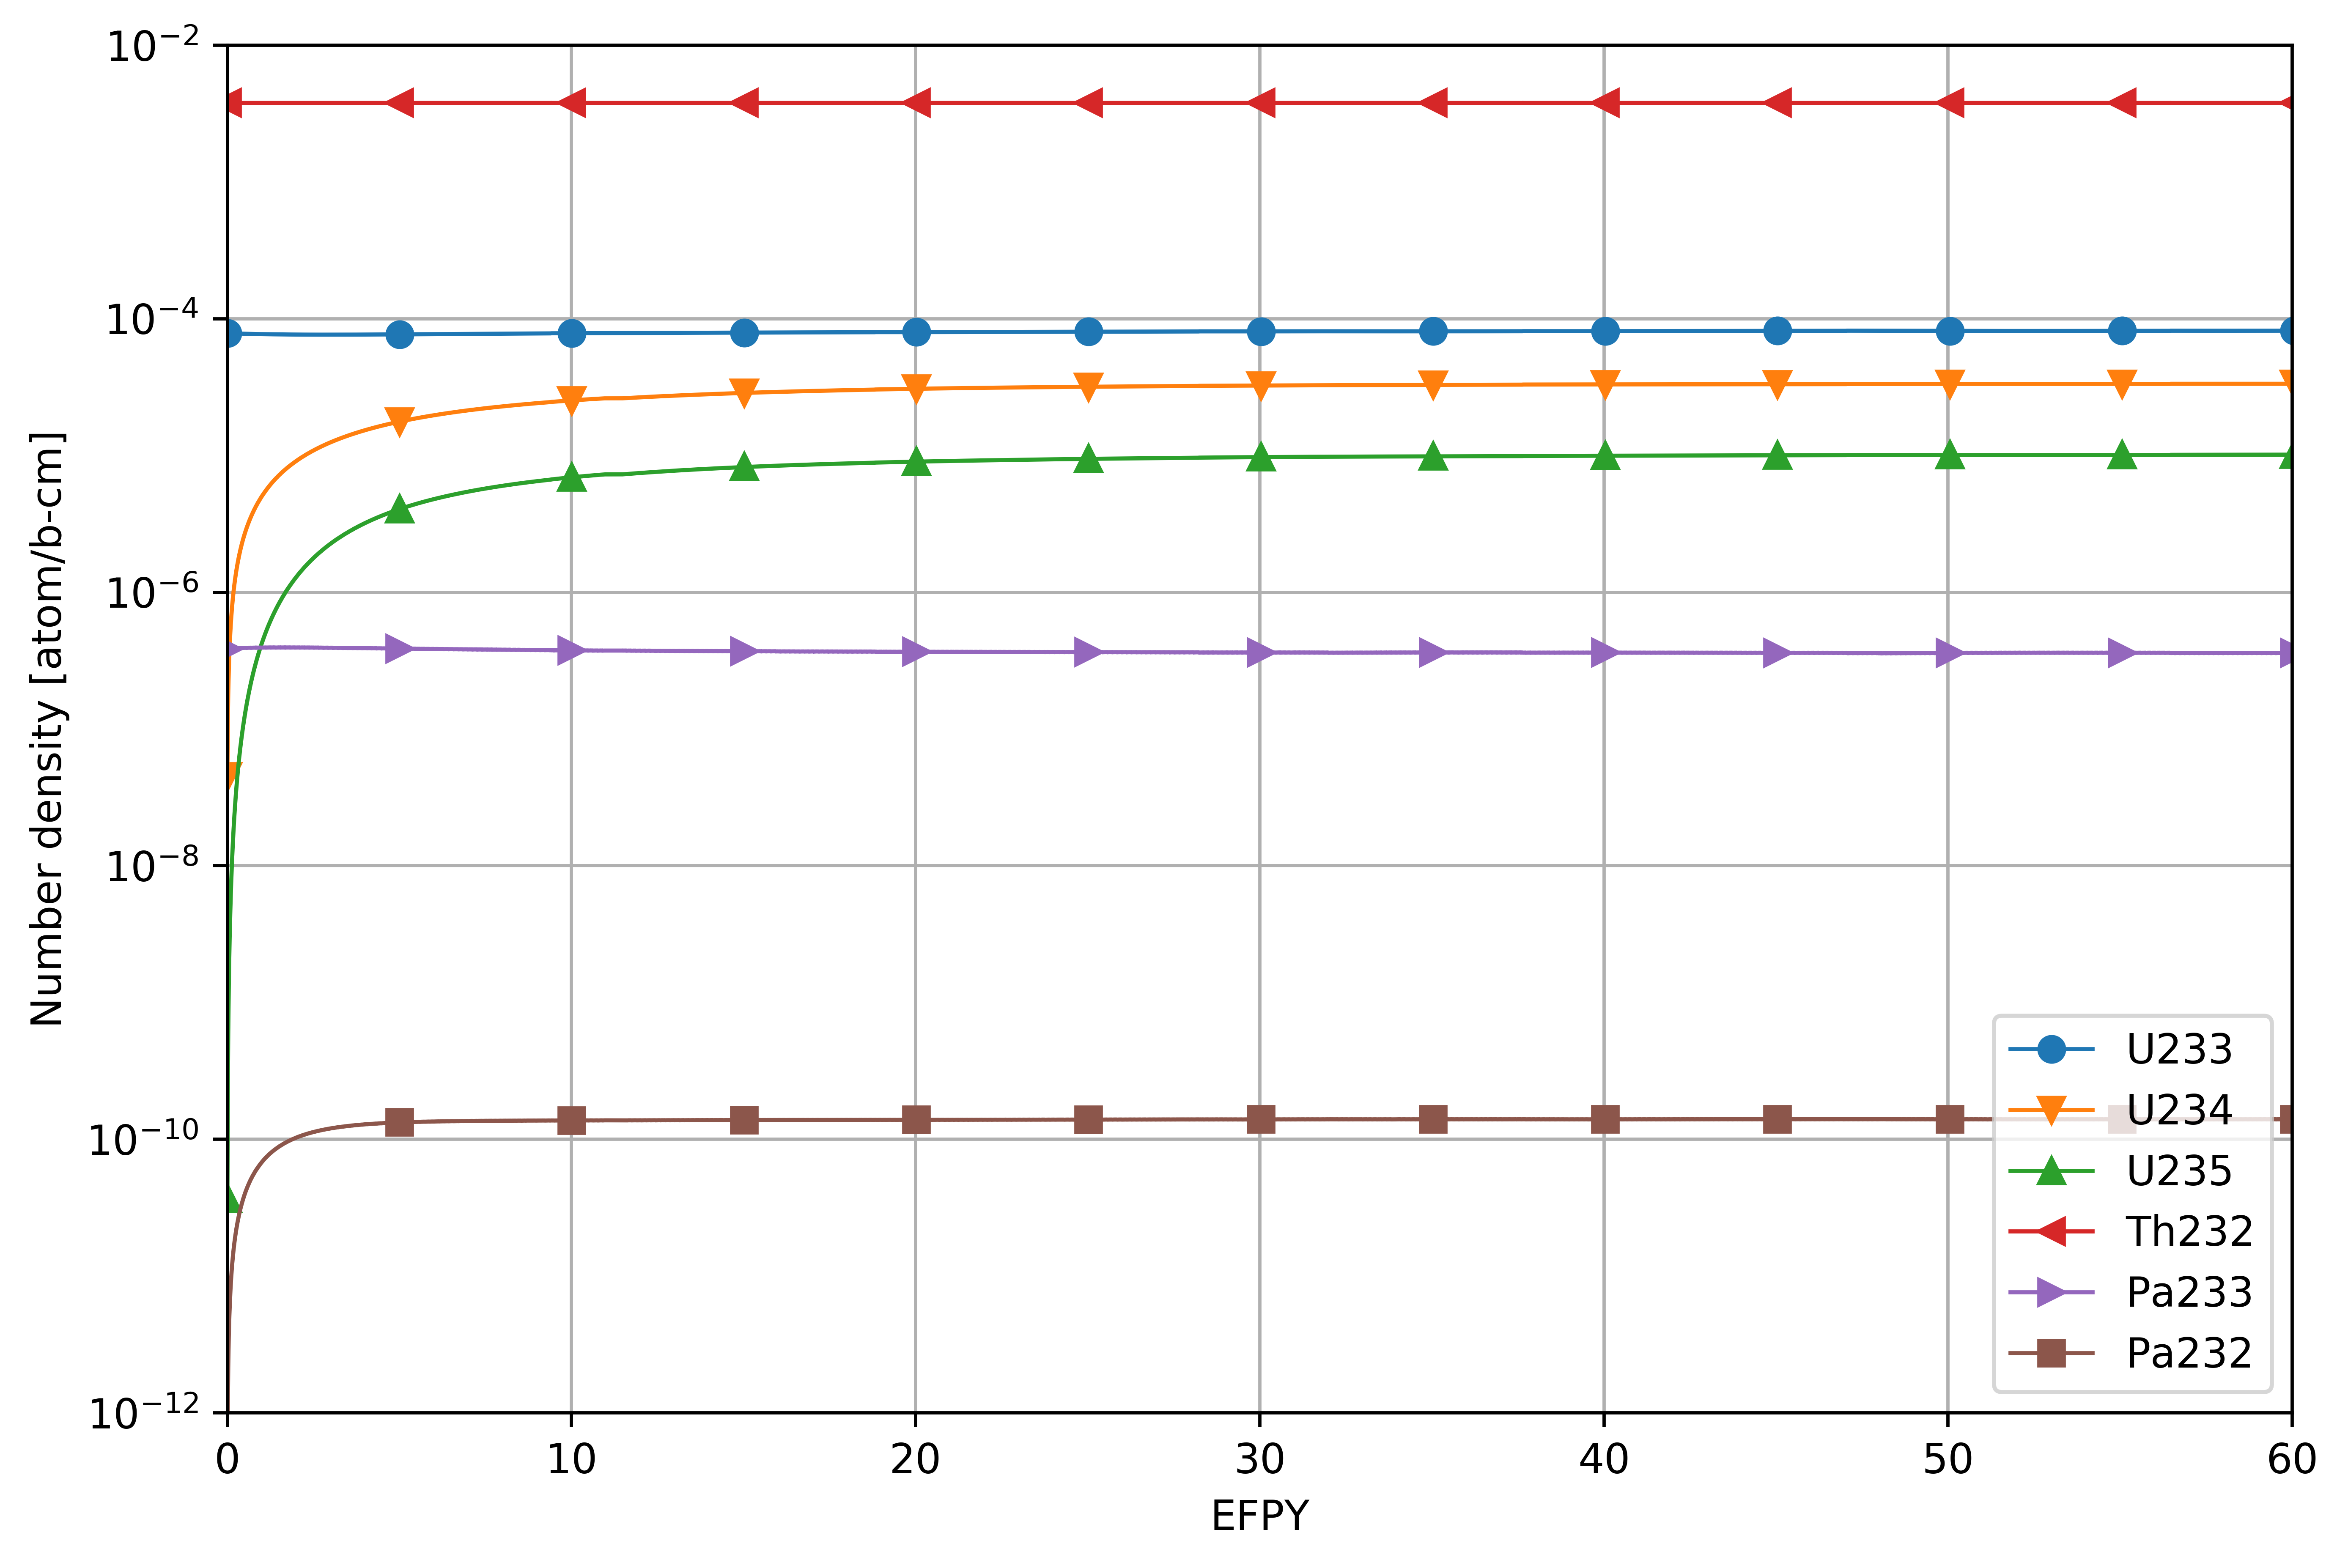
\includegraphics[width=\textwidth]{major_isotopes_adens.png}
  \caption{Number density of major nuclides during 60 years of reactor 
  operation.}
  \label{fig:adens_eq}
\end{figure}
In contrast, a wide variety of nuclides, including fissile isotopes (e.g. 
$^{235}$U) and non-fissile strong absorbers (e.g. $^{234}$U), kept accumulating 
in the core. Figure~\ref{fig:fissile_short} demonstrates production of fissile 
isotopes in the core. In the end of the considered operational time, the core 
contained significant $^{235}$U ($\approx10^{-5}$ atom/b-cm), $^{239}$Pu 
($\approx5\times10^{-7}$ atom/b-cm), and $^{241}$Pu ($\approx 5\times10^{-7}$ 
atom/b-cm). Meanwhile, the equilibrium number density of the target fissile 
isotope $^{233}$U was approximately 7.97$\times10^{-5}$ atom/b-cm. Small dips 
in neptunium and plutonium number density every 16 years are caused by removing
$^{237}$Np and $^{242}$Pu (included in Processing group ``Higher nuclides'', see
 Table~\ref{tab:reprocessing_list}) which decay into $^{235}$Np and $^{239}$Pu, 
 respectively. Thus, 
production of new fissile materials in the core, as well as $^{233}$U breeding, 
made it possible to compensate for negative effects of strong absorber 
accumulation and keep the reactor critical.
\begin{figure}[htp!] % replace 't' with 'b' to 
  \centering
  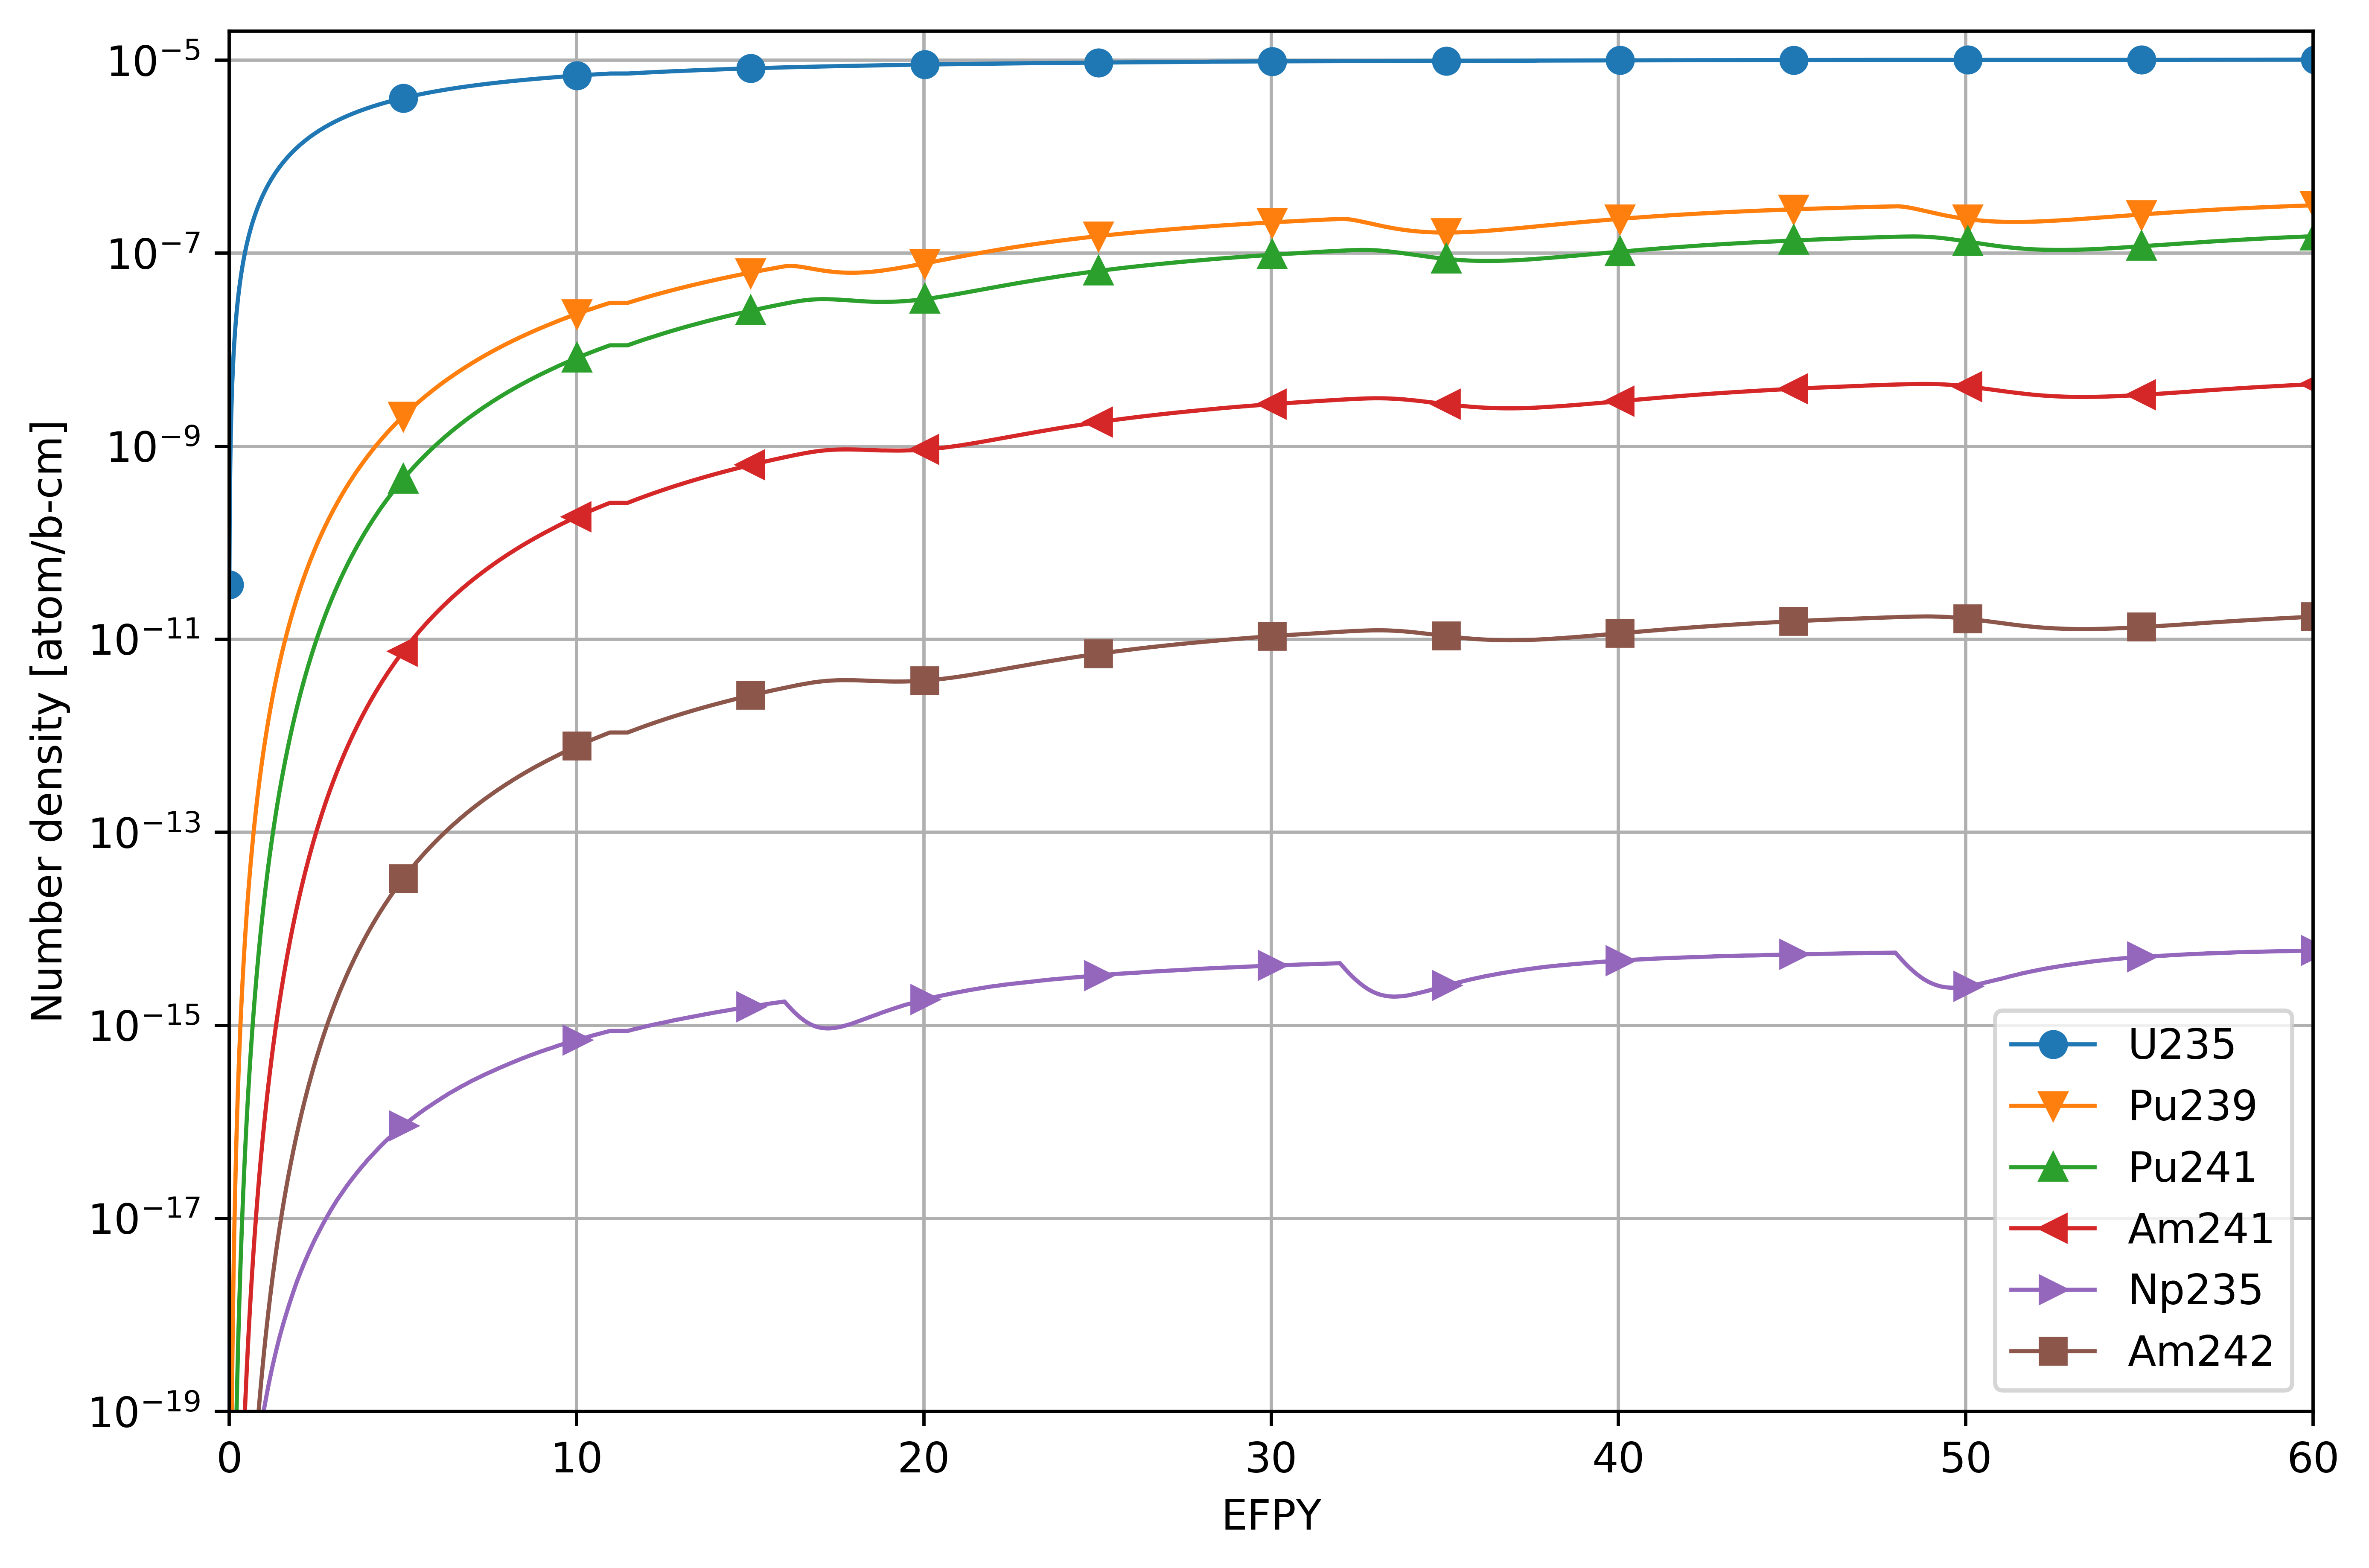
\includegraphics[width=\textwidth]{fissile_short.png}
  \caption{Number density of fissile in epithermal spectrum nuclides 
  accumulation during the reactor operation.}
  \label{fig:fissile_short}
\end{figure}

\subsection{Neutron spectrum}
Figure~\ref{fig:spectrum} shows the normalized neutron flux spectrum for the 
full-core \gls{MSBR} model in the energy range from $10^{-8}$ to $10$ MeV. The 
neutron energy spectrum at equilibrium is harder than at startup due to 
plutonium and other strong absorbers accumulating in the core during reactor 
operation.  
\begin{figure}[ht!] % replace 't' with 'b'         to force it to 
  \centering
  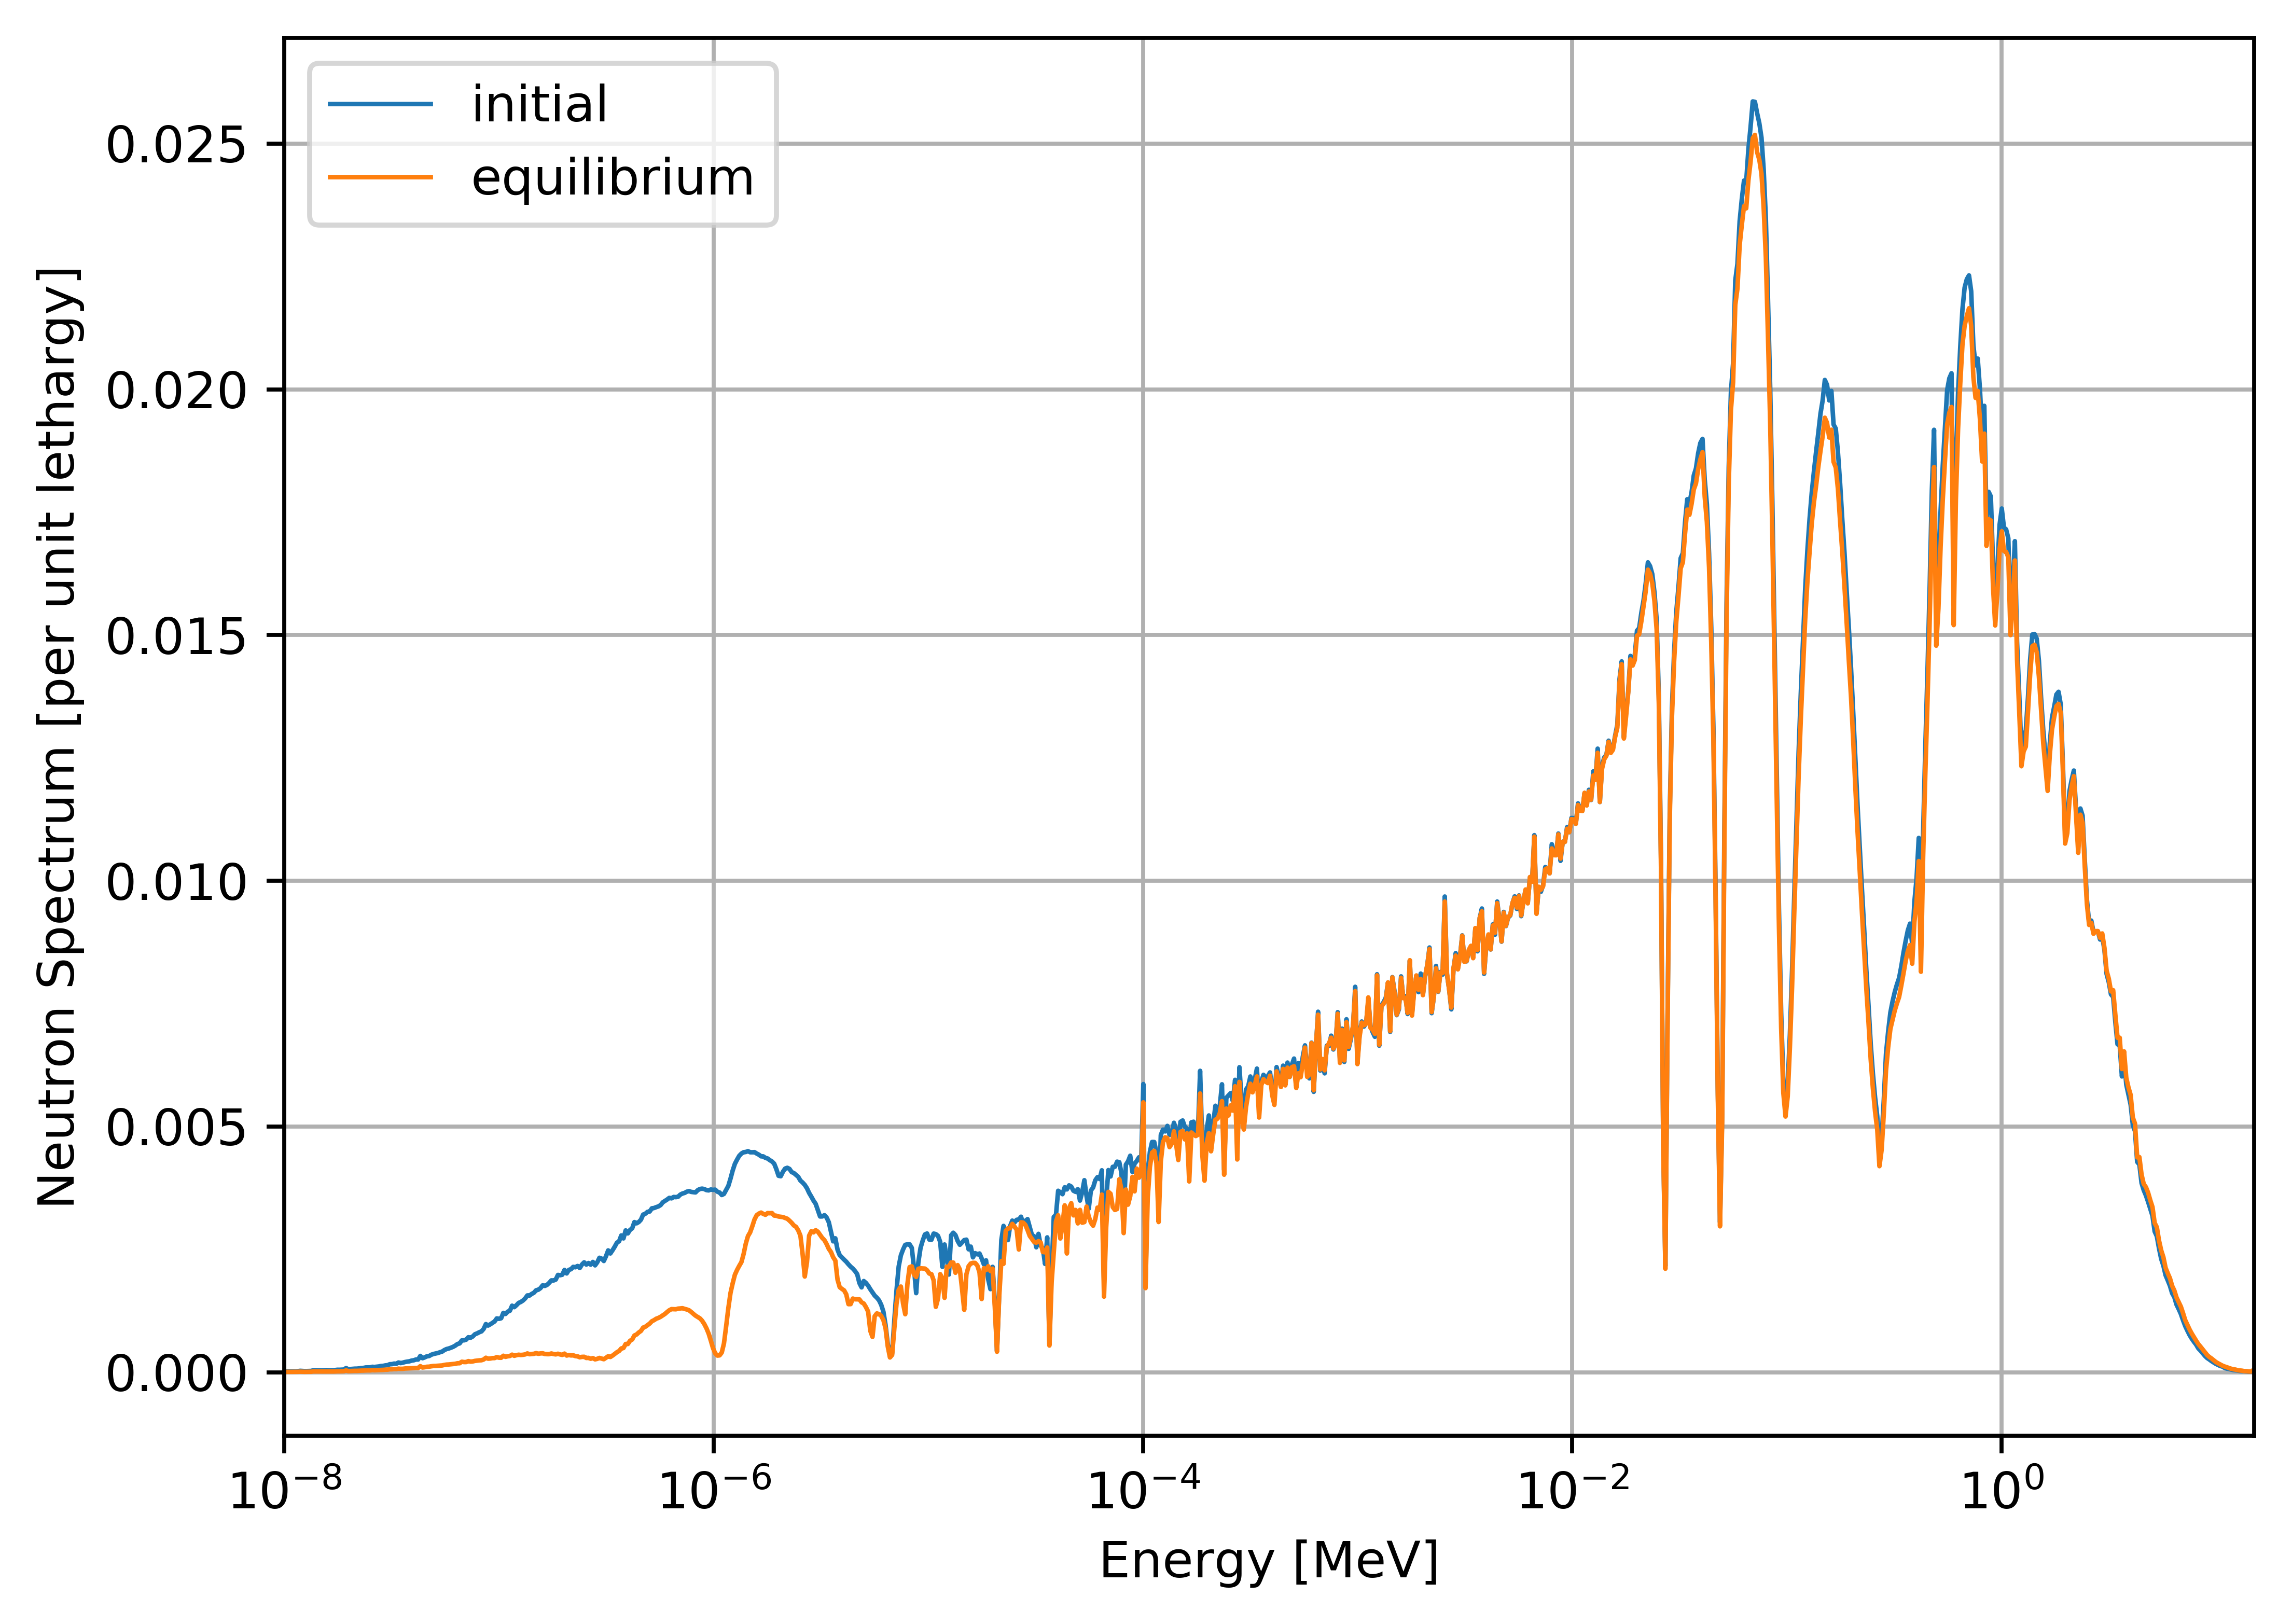
\includegraphics[width=\textwidth]{spectrum.png} \caption{The neutron flux energy 
  spectrum is normalized by unit lethargy and the area under the curve is normalized to 1 for initial and equilibrium fuel salt 
  composition.}
  \label{fig:spectrum}
\end{figure}

Figure~\ref{fig:spectrum_zones} shows that zone I produced more thermal neutrons 
than zone II, corresponding to a majority of fissions occurring in the central part 
of the core. In the undermoderated zone II, the neutron energy spectrum is harder, 
which leads to more neutrons capture by $^{232}$Th and helps achieve relatively 
high breeding ratio. Moreover, the (n,$\gamma$) resonance energy range in $^{232}$Th 
is from 10$^{-4}$ to 10$^{-2}$ MeV. Therefore, the moderator-to-fuel ratio for zone 
II was chosen to shift the neutron energy spectrum in this range. Furthermore, in the 
central core region (zone I), the neutron energy spectrum shifts to a harder spectrum 
over 20 years of reactor operation. Meanwhile, in the outer core region (zone II), a 
similar spectral shift takes place at a reduced scale. These results are in a good 
agreement with original ORNL report \cite{robertson_conceptual_1971} and the most recent 
whole-core steady-state study \cite{park_whole_2015}.

It is important to obtain the epithermal and thermal spectra to produce $^{233}$U from 
$^{232}$Th because the radiative capture cross section of thorium decreases monotonically 
from $10^{-10}$ MeV to $10^{-5}$ MeV. Hardening the spectrum tends to significantly 
increase resonance absorption in thorium and decrease absorptions in fissile and 
construction materials. 
\begin{figure}[ht!] % replace 't' with 'b' to force it to 
  \centering
  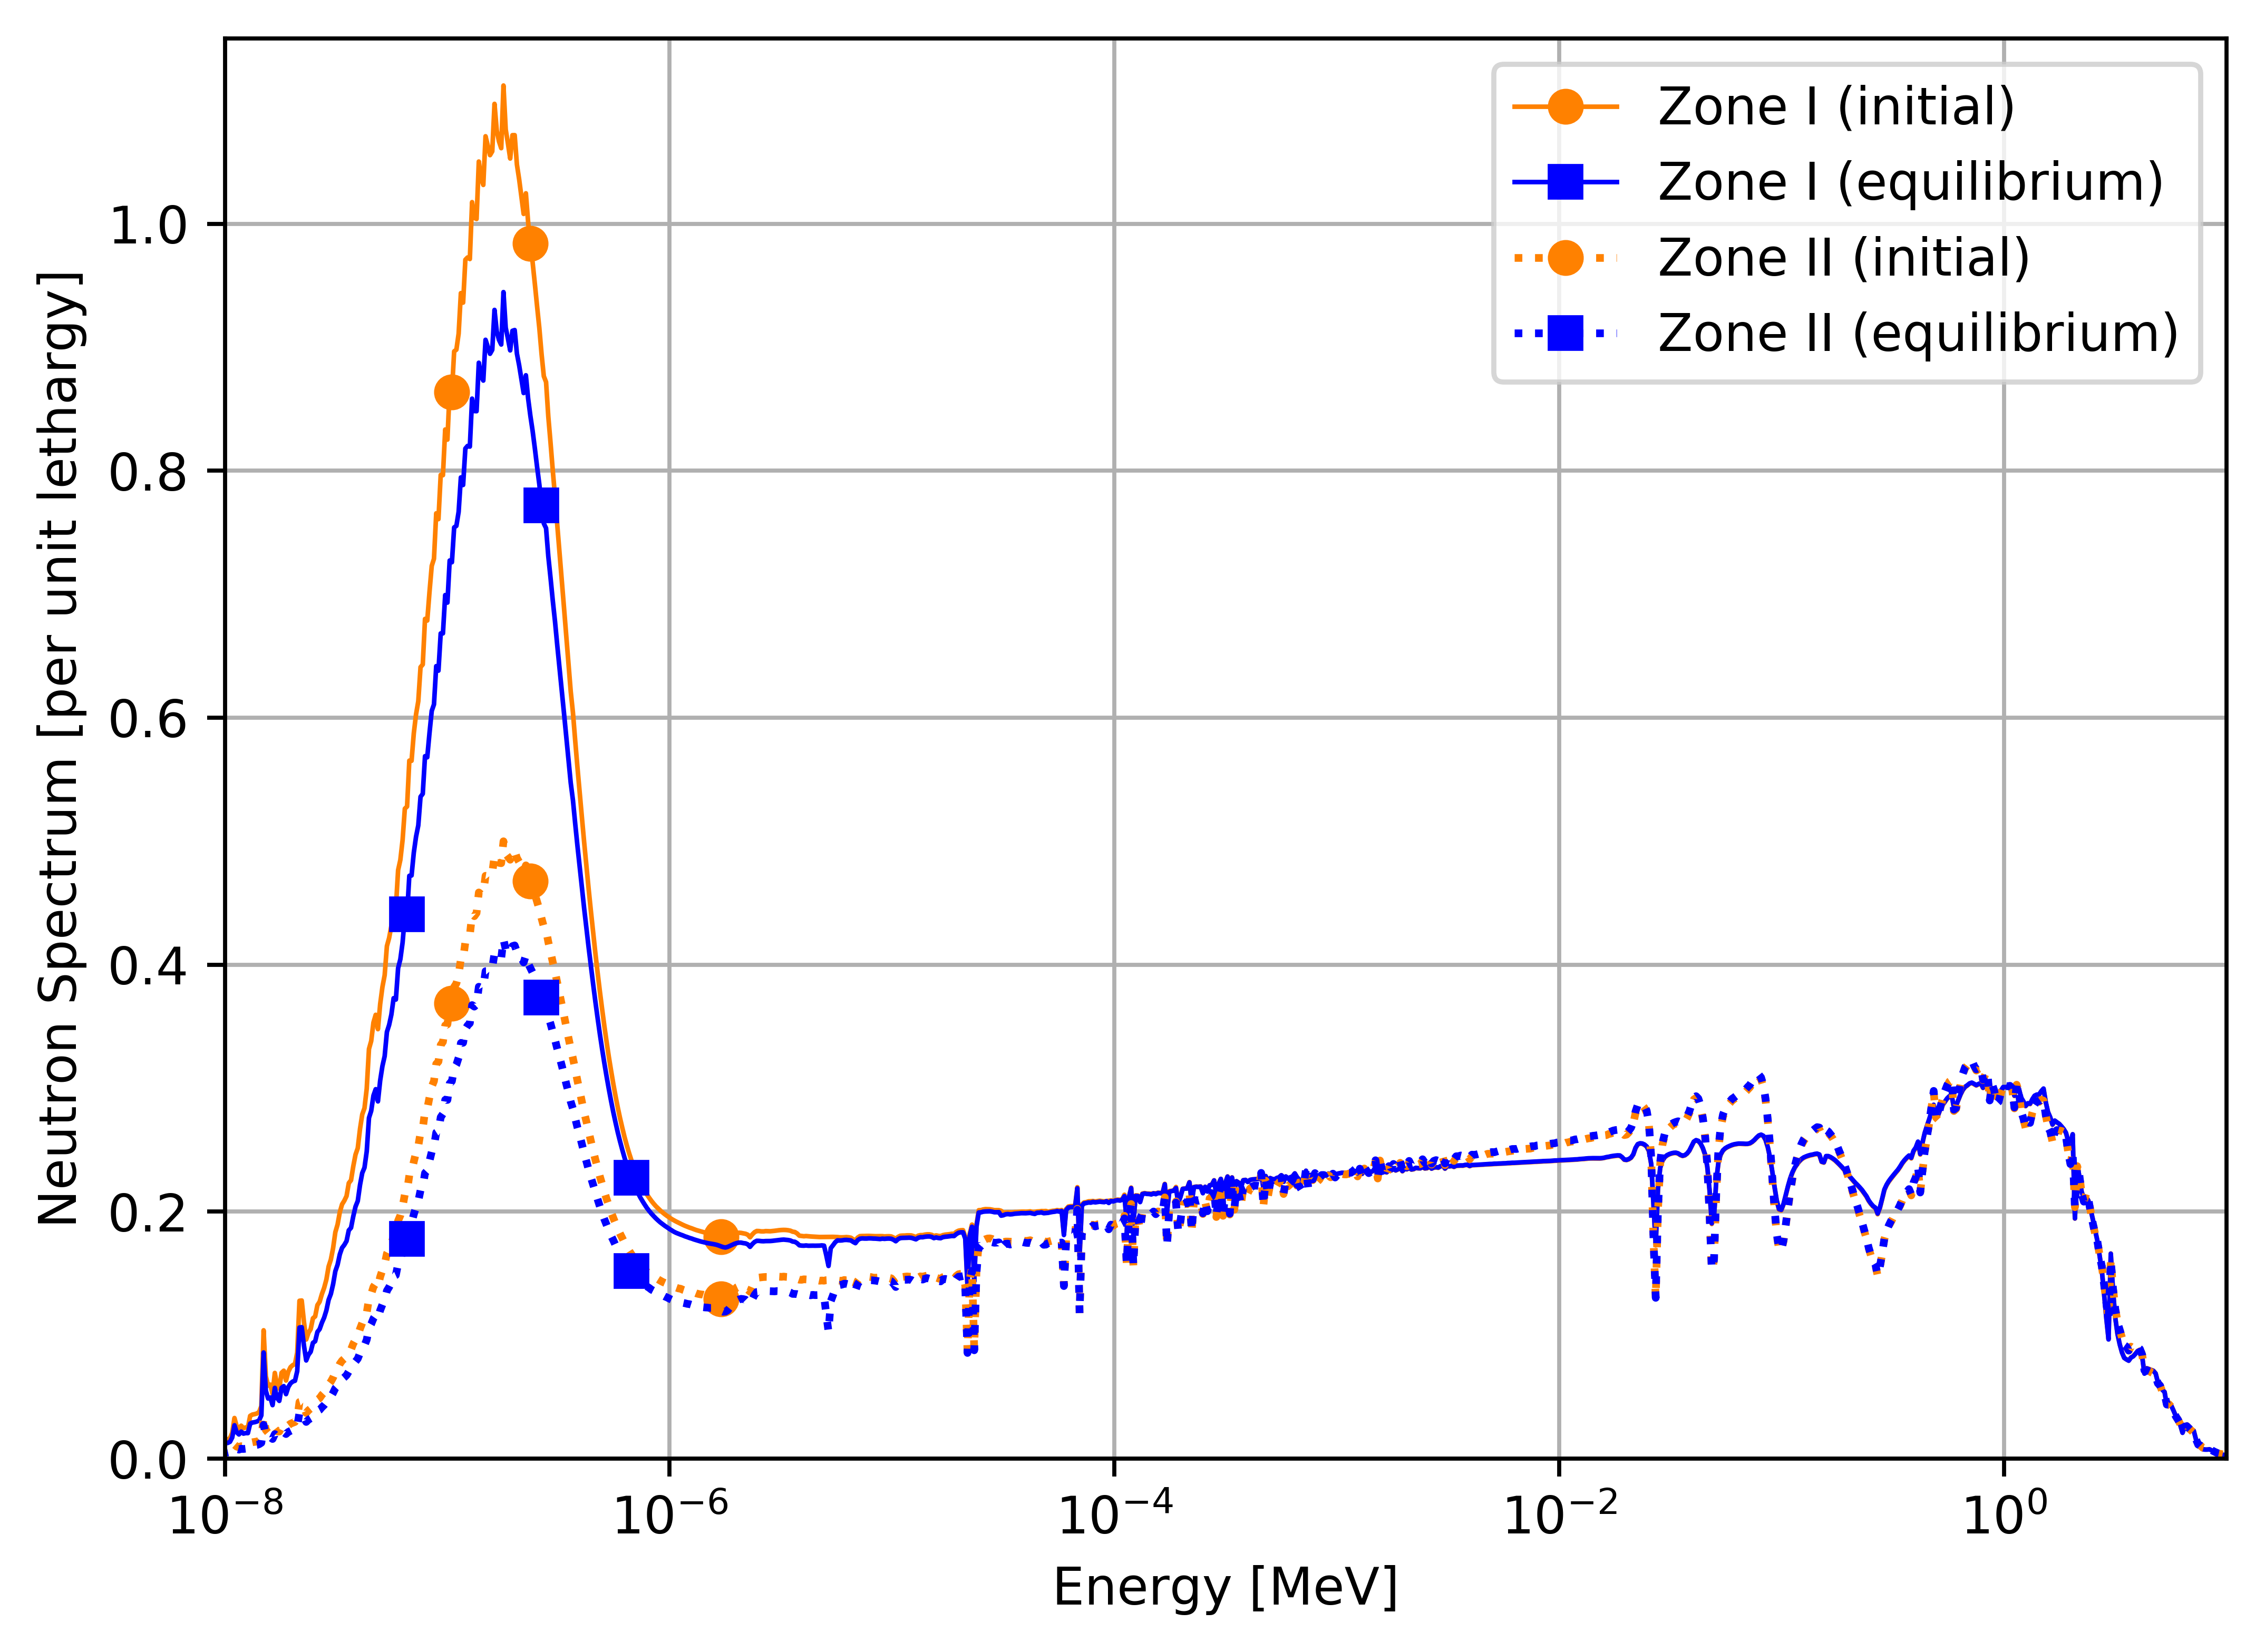
\includegraphics[width=\textwidth]{spectrum_zones.png} 
  \caption{The neutron flux energy spectrum in different core regions is normalized by 
unit lethargy and the area under the curve is normalized to 1 for the initial and equilibrium fuel salt composition.}
  \label{fig:spectrum_zones}
\end{figure}

\subsection{Neutron flux}
Figure~\ref{fig:radial_flux} shows the radial distribution of fast and thermal 
neutron flux for the both initial and equilibrium composition. The neutron fluxes
have similar shapes for both compositions but the equilibrium case has a harder 
spectrum. A significant spectral shift was observed in the central region of 
the core (zone I), while for the outer region (zone II), it is negligible for fast 
but notable for thermal neutrons. These neutron flux radial distributions 
agree with the fluxes in the original ORNL report \cite{robertson_conceptual_1971}. 
Overall, spectrum hardening during \gls{MSBR} operation should be carefully 
studied when designing the reactivity control system.
\begin{figure}[ht!] % replace 't' with 'b' to force it to \centering
  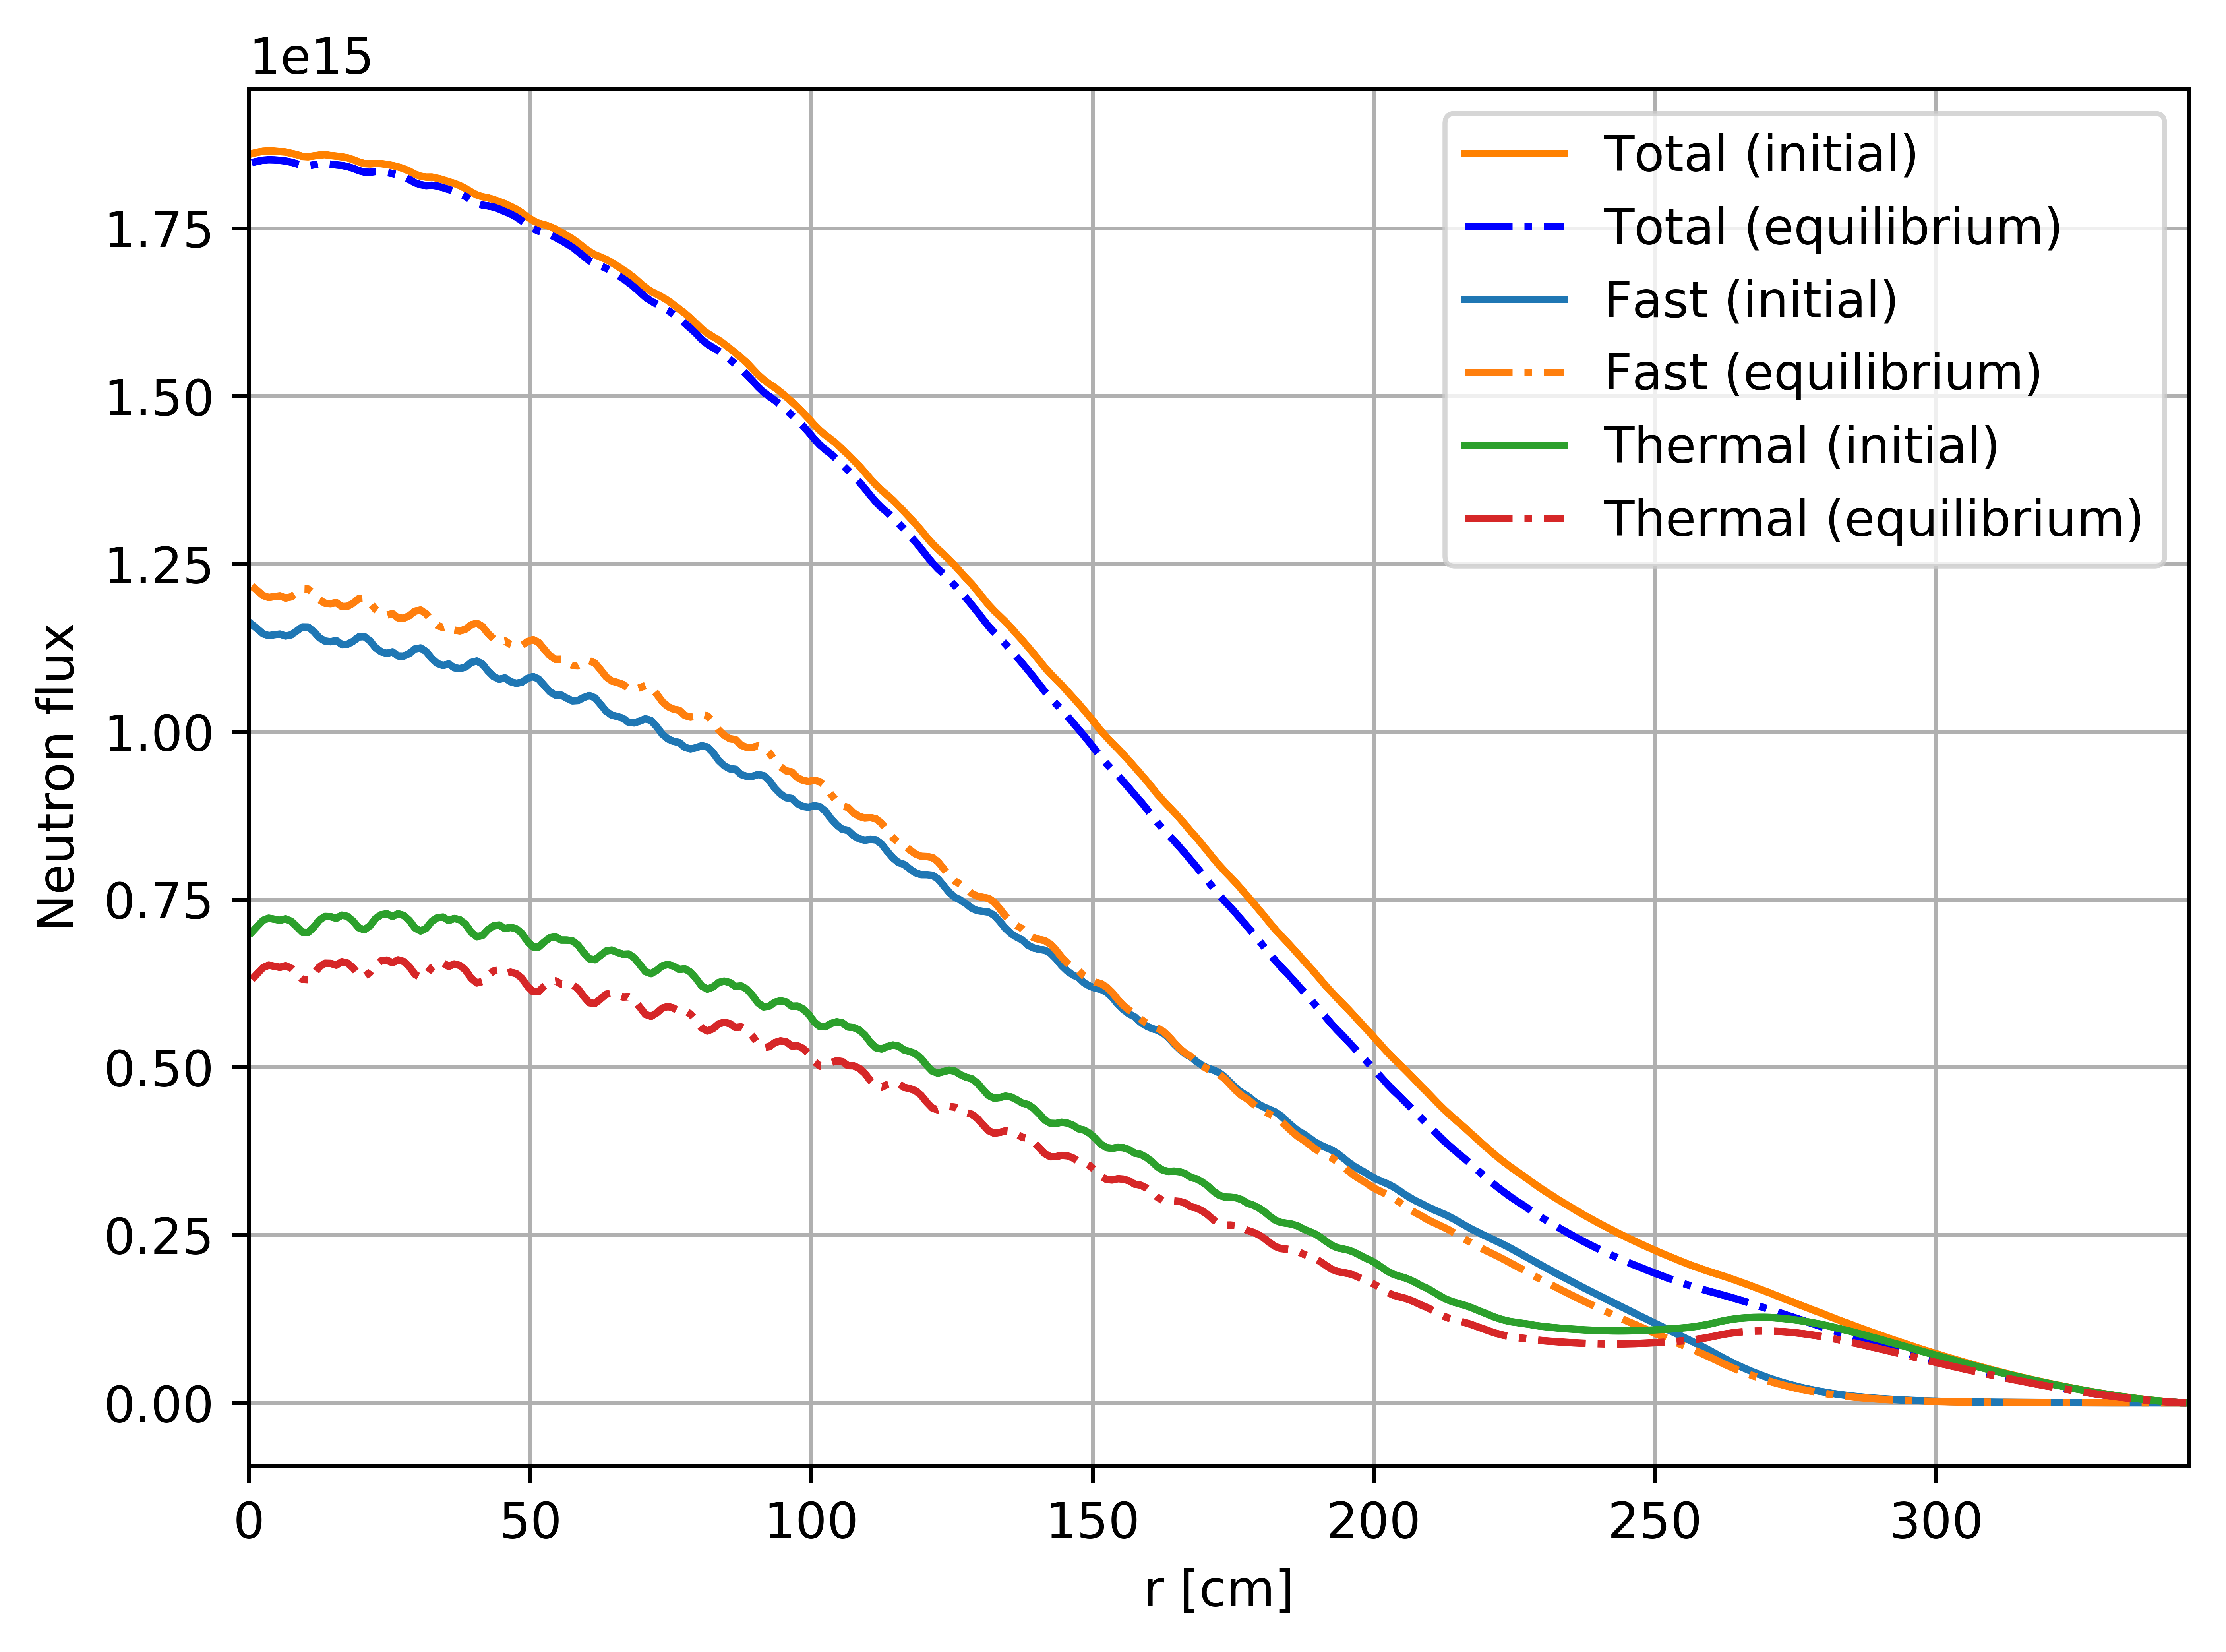
\includegraphics[width=\textwidth]{radial_flux.png} \caption{Radial neutron 
  flux distribution for initial and equilibrium fuel salt composition.}
  \label{fig:radial_flux}
\end{figure}

\subsection{Power and breeding distribution}
Table~\ref{tab:powgen_fraction} shows the power fraction in each zone for 
initial and equilibrium fuel compositions. Figure~\ref{fig:pow_den} reflects the 
normalized power distribution of the \gls{MSBR} quarter core for equilibrium fuel
 salt composition. For both the initial and equilibrium compositions, fission 
primarily occurs in the center of the core, namely zone I. The spectral shift 
during reactor operation results in slightly different power fractions at startup and 
equilibrium, but most of the power is still generated in zone I at equilibrium 
(table~\ref{tab:powgen_fraction}). 
%%%%%%%%%%%%%%%%%%%%%%%%%%%%%%%%%%%%%%%%
\begin{table}[ht!]
  \caption{Power generation fraction in each zone for initial and equilibrium 
  state.}
\begin{tabularx}{\textwidth}{ m | s | s } \hline
Core region      & Initial      & Equilibrium   \\   \hline
Zone I           & 97.91\%      & 98.12\%   \\
Zone II          & 2.09\%       & 1.88\%   \\ \hline
\end{tabularx}
  \label{tab:powgen_fraction}
\end{table}
%%%%%%%%%%%%%%%%%%%%%%%%%%%%%%%%%%%%%%%%%%%%%%%%%%%%%%%%%%%%%%%%%%%%%%%%%%%%%%%%
Figure~\ref{fig:breeding_den} shows the neutron capture reaction rate 
distribution for $^{232}$Th normalized by the total neutron flux for initial 
and equilibrium states. The distribution reflects the spatial distribution of 
$^{233}$U production in the core. $^{232}$Th 
neutron capture produces $^{233}Th$ which then $\beta$-decays to 
$^{233}$Pa, the precursor for $^{233}$U production. Accordingly, this 
characteristic represents the breeding distribution in the \gls{MSBR} core. 
Spectral shift does not cause significant changes in power nor in breeding 
distribution. Even after 20 years of operation, most of the power is still 
generated in zone I.
\begin{figure}[ht!] % replace 't' with 'b' to force it to \centering
  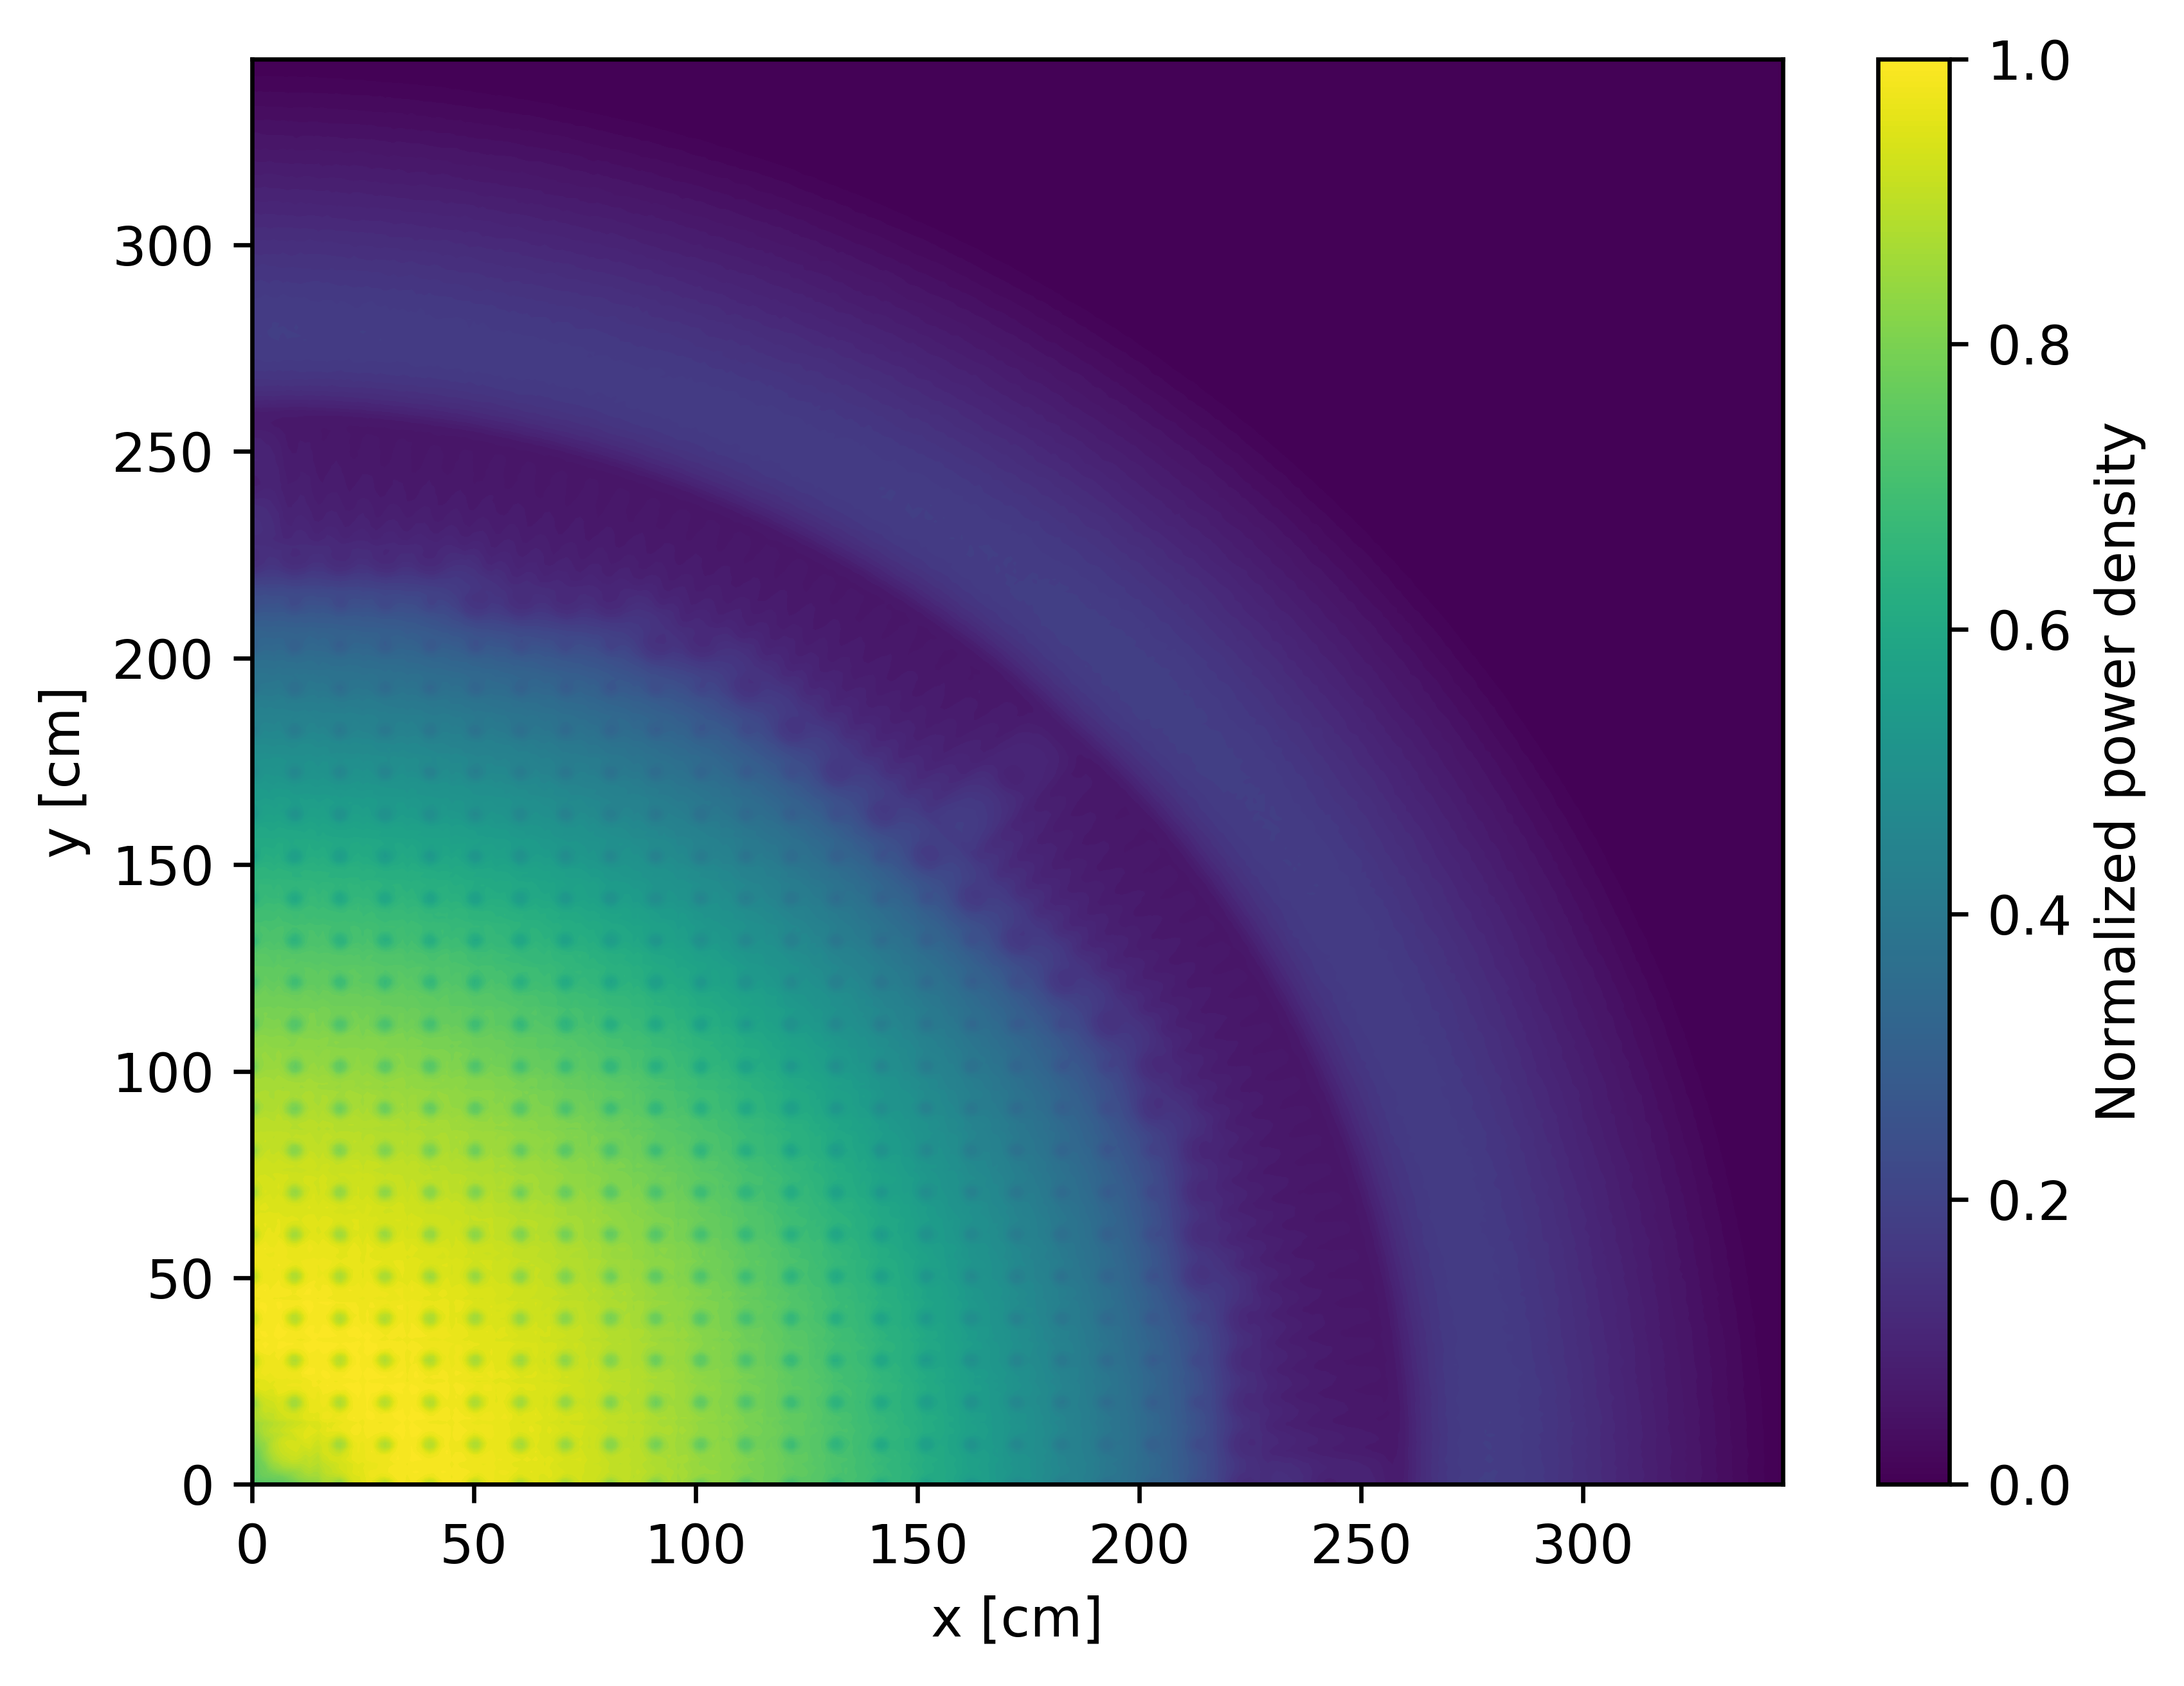
\includegraphics[width=\textwidth]{power_distribution_eq.png} 
  \caption{Normalized power density for equilibrium fuel salt 
  composition.}
  \label{fig:pow_den}
\end{figure}
\begin{figure}[ht!] % replace 't' with 'b' to force it to \centering
  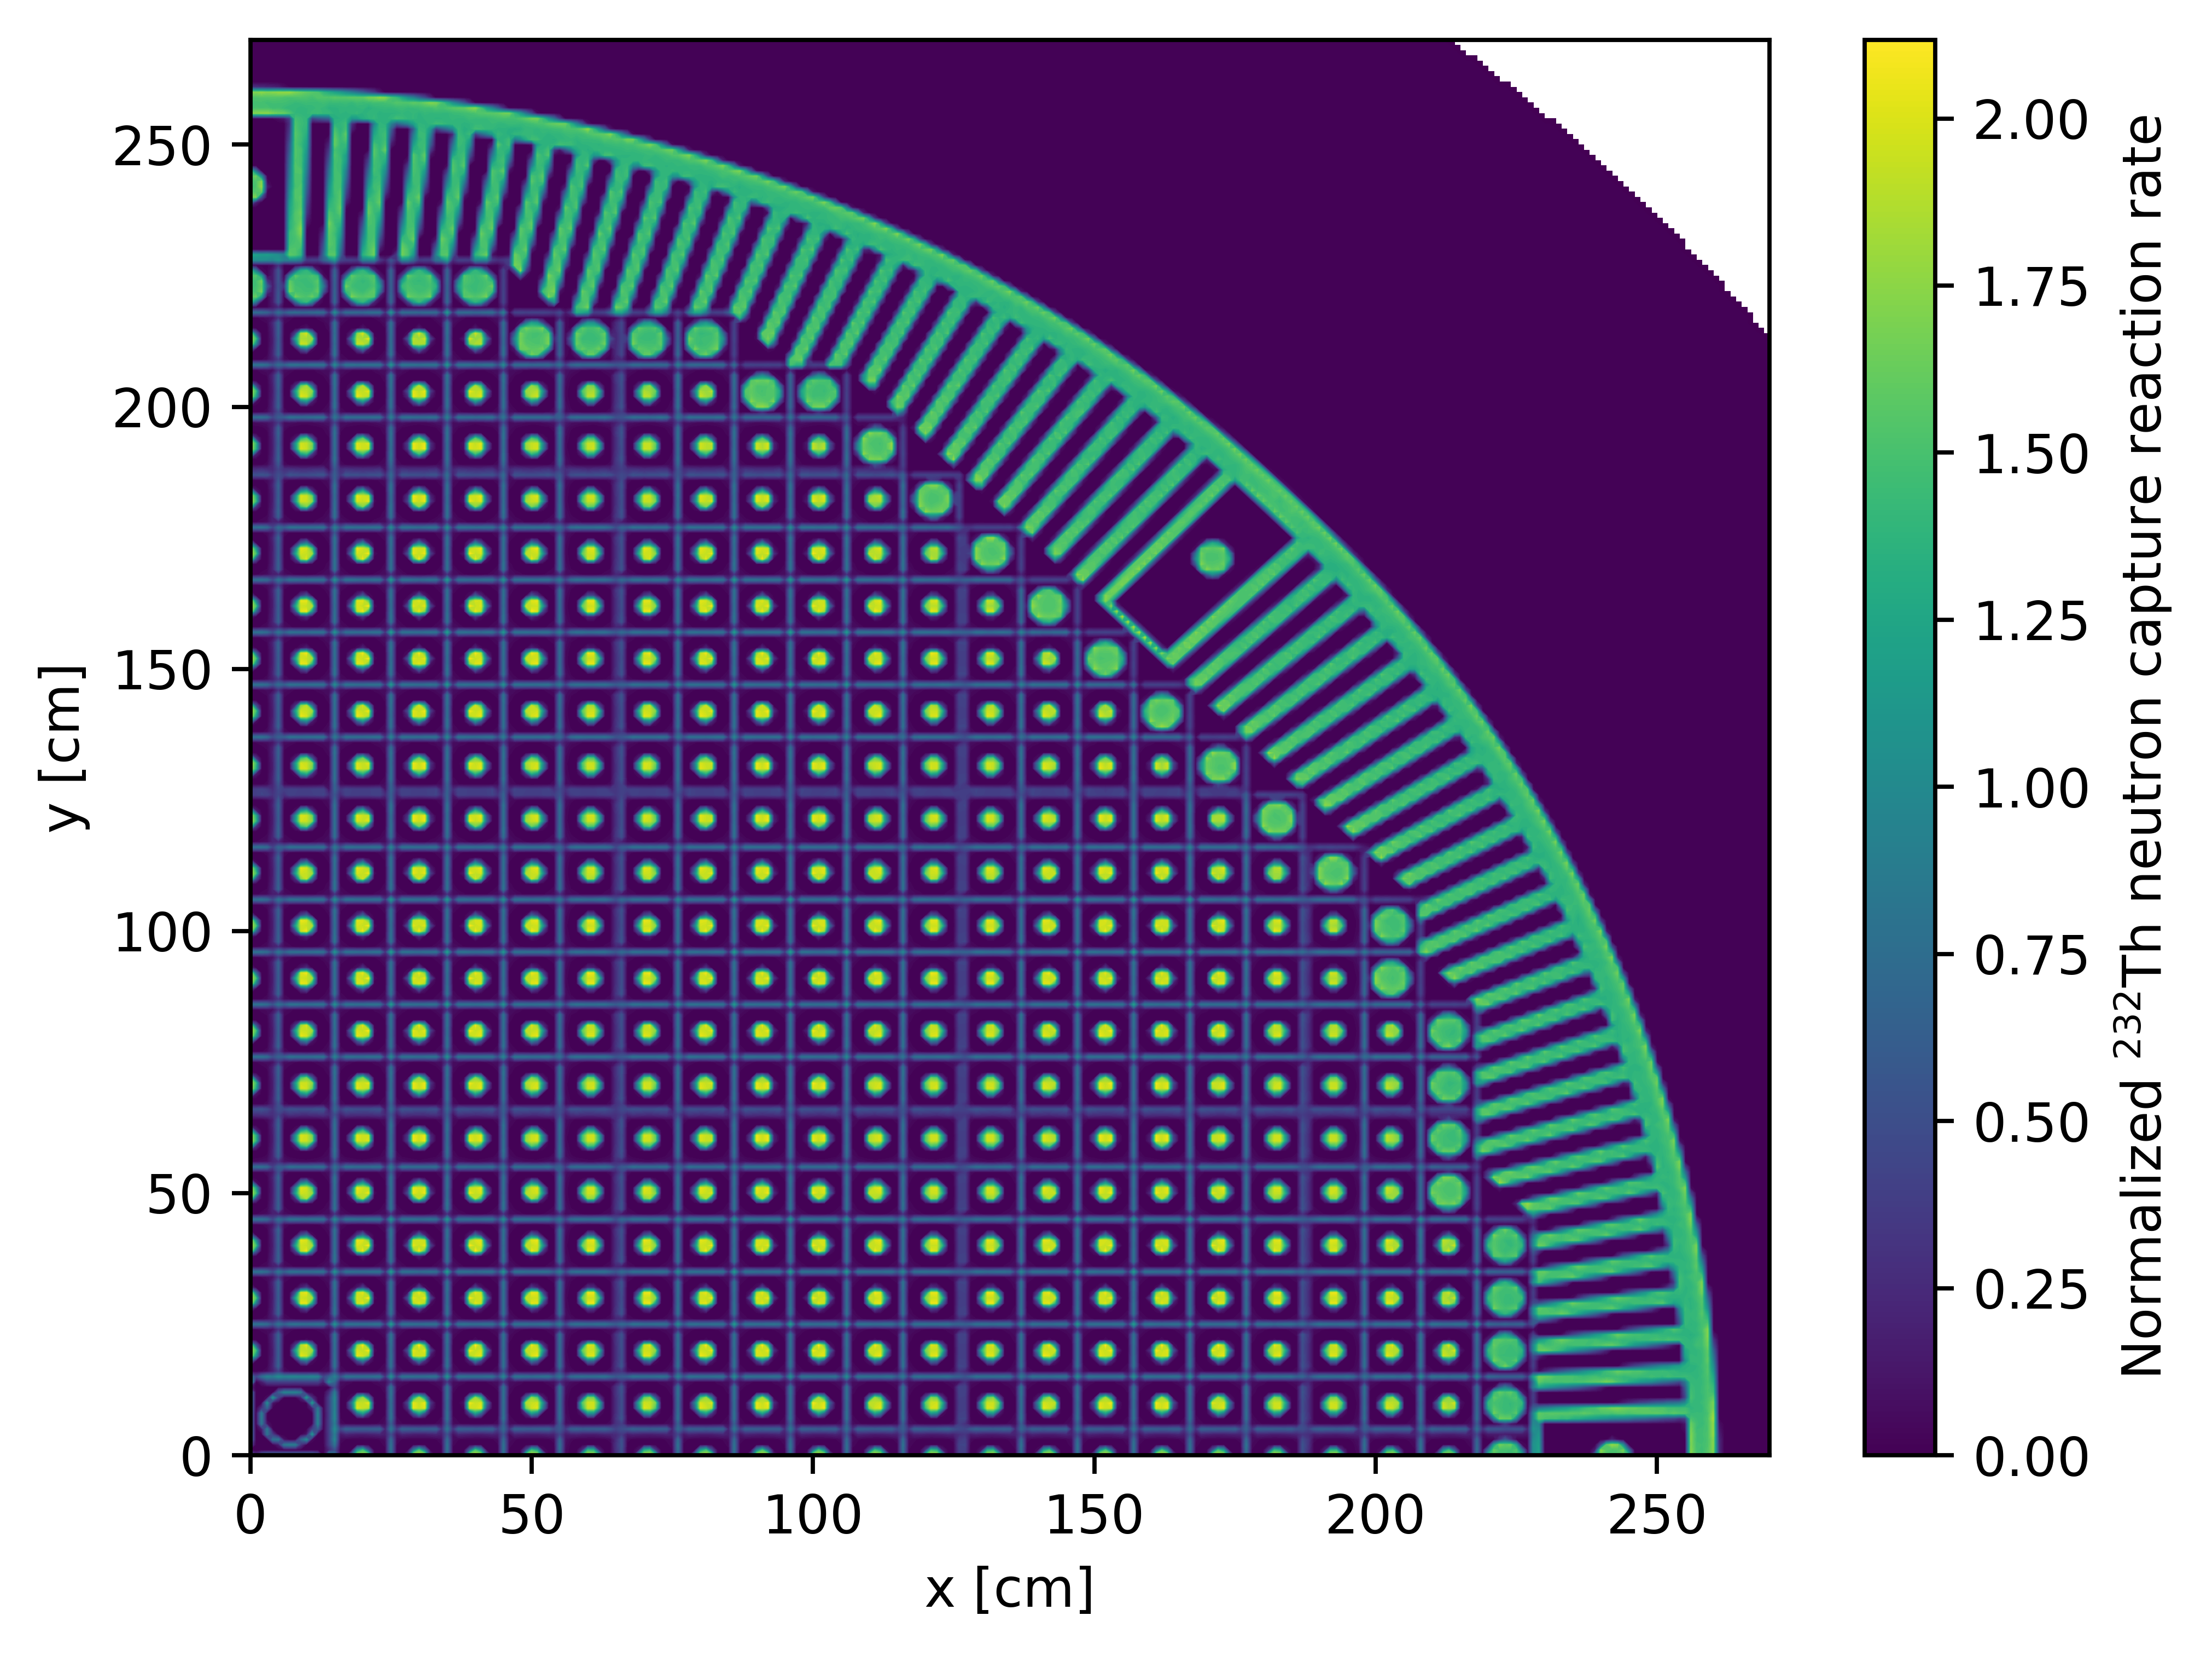
\includegraphics[width=\textwidth]{breeding_distribution_eq.png} 
  \caption{$^{232}$Th neutron capture reaction rate normalized by total flux 
  for equilibrium fuel salt composition.}
  \label{fig:breeding_den}
\end{figure}
\subsection{Temperature coefficient of reactivity}
Table~\ref{tab:tcoef} summarizes temperature effects on reactivity calculated 
in this work for both initial and equilibrium fuel compositions, compared 
with the original \gls{ORNL} report data \cite{robertson_conceptual_1971}. 
By propagating the $k_{eff}$  statistical error provided by SERPENT2, 
uncertainty for each temperature coefficient was obtained and appears in 
Table~\ref{tab:tcoef}. Other sources of uncertainty are neglected, such as cross section 
measurement error and approximations inherent in the equations of state 
providing both the salt and graphite density dependence on temperature.
 The main physical principle underlying the reactor 
temperature feedback is an expansion of heated material. When the fuel 
salt temperature increases, the density of the salt decreases, but at the same 
time, the total volume of fuel salt in the core remains constant because it is 
bounded by the graphite. When the graphite temperature increases, the density 
of graphite decreases, creating additional space for fuel salt. To determine 
the temperature coefficients, the cross section temperatures for the fuel and 
moderator were changed from 900K to 1000K. Three different cases were considered:
\begin{enumerate}
  \item Temperature of fuel salt rising from 900K to 1000K.
  \item Temperature of graphite rising from 900K to 1000K.
  \item Whole reactor temperature rising from 900K to 1000K.
\end{enumerate}
%%%%%%%%%%%%%%%%%%%%%%%%%%%%%%%%%%%%%%%%
\begin{table}[ht!]
  \caption{Temperature coefficients of reactivity for initial and equilibrium 
  state.}
\begin{tabularx}{\textwidth}{ X | r | r | r } \hline
Reactivity coefficient               & Initial         & Equilibrium     & Reference                                 \\ 
                                        & [pcm/k]         &  [pcm/k]        & (initial)\cite{robertson_conceptual_1971} \tabularnewline  \hline
Doppler in fuel salt                    & $-4.73\pm0.038$ & $-4.69\pm0.038$ & $-4.37$  \tabularnewline
Fuel salt density                       & $+1.21\pm0.038$ & $+1.66\pm0.038$ & $+1.09$  \tabularnewline
Total fuel salt                         & $-3.42\pm0.038$ & $-2.91\pm0.038$ & $-3.22$  \tabularnewline \hline
Graphite spectral shift                 & $+1.56\pm0.038$ & $+1.27\pm0.038$ &          \tabularnewline
Graphite density                        & $+0.14\pm0.038$ & $+0.23\pm0.038$ &          \tabularnewline
Total moderator (graphite)              & $+1.69\pm0.038$ & $+1.35\pm0.038$ & $+2.35$  \tabularnewline \hline
Total core                              & $-1.64\pm0.038$ & $-1.58\pm0.038$ & $-0.87$  \tabularnewline \hline
\end{tabularx}
  \label{tab:tcoef}
\end{table}
%%%%%%%%%%%%%%%%%%%%%%%%%%%%%%%%%%%%%%%%%%%%%%%%%%%%%%%%%%%%%%%%%%%%%%%%%%%%%%%%
In the first case, changes in the fuel temperature only impact fuel density. In 
this case, the geometry is unchanged because the fuel is a liquid. However, 
when the moderator heats up, both the density and the geometry change due to 
thermal expansion of the solid graphite blocks and reflector. Accordingly, the 
new graphite density was calculated using a linear temperature expansion 
coefficient of 1.3$\times10^{-6}$K$^{-1}$ \cite{robertson_conceptual_1971}. A new 
geometry input for SERPENT2, which takes into account displacement of graphite 
surfaces, was created based on this information. For calculation of 
displacement, it was assumed that the interface between the graphite reflector and vessel did not move,
 and that the vessel temperature did not change. This is the most reasonable assumption for
 the short-term reactivity effects because inlet salt is cooling graphite reflector and 
inner surface of the vessel.

The fuel temperature coefficient (FTC) is negative for both initial and 
equilibrium fuel compositions due to thermal Doppler broadening of the resonance 
capture cross sections in the thorium. A small positive effect of fuel density on 
reactivity increases from $+1.21$ pcm/K at reactor startup to $+1.66$ pcm/K for 
equilibrium fuel composition which has a negative effect on FTC magnitude during the 
reactor operation. This is in good agreement with earlier 
research \cite{robertson_conceptual_1971,park_whole_2015}. The moderator 
temperature coefficient (MTC) is positive for the startup composition and decreases 
during reactor operation because of spectrum hardening with fuel depletion. 
Finally, the total temperature coefficient of reactivity is negative for both 
cases, but decreases during reactor operation due to spectral shift. In 
summary, even after 20 years of operation the total temperature coefficient of 
reactivity is relatively large and negative during reactor operation (comparing 
with conventional PWR which has temperature coefficient about -1.71 pcm/$^\circ$F 
$\approx$ -3.08 pcm/K \cite{forget_integral_2018}), despite positive MTC, and 
affords excellent reactor stability and control.

\subsection{Reactivity control system rod worth}
Table~\ref{tab:rod_worth} summarizes the reactivity control system worth. 
During normal operation, the control (graphite) rods are fully inserted, and the 
safety (B$_4$C) rods are fully withdrawn. To insert negative reactivity into 
the core, the graphite rods are gradually withdrawn from the core. In an 
accident, the safety rods would be dropped down into the core. The integral rod 
worths were calculated for various positions to separately estimate the worth
of the control graphite rods\footnote{In \cite{robertson_conceptual_1971}, the 
graphite rods are referred to as ``control'' rods.}, the safety (B$_4$C) rods, 
and the whole reactivity control system. Control rod integral worth is 
approximately 28 cents and stays almost constant during reactor operation. The 
safety rod integral worth decreases by  16.2\% during 20 years of operation 
because of neutron spectrum hardening and absorber accumulation in proximity to 
reactivity control system rods. This 16\% decline in control system worth 
should be taken into account in \gls{MSBR} accident analysis and safety 
justification.
%%%%%%%%%%%%%%%%%%%%%%%%%%%%%%%%%%%%%%%%
\begin{table}[ht!]
  \caption{Control system rod worth for initial and equilibrium fuel 
  composition.}
\begin{tabularx}{\textwidth}{ b | x | x } \hline
Reactivity parameter [cents]  &  Initial      &  Equilibrium      \\ \hline
Control (graphite) rod integral worth               & $\ 28.2\pm0.8$    & $\ 
        29.0\pm0.8$ \\ Safety (B$_4$C) rod integral worth                  & 
        $251.8\pm0.8$    & $211.0\pm0.8$  \\
Total reactivity control system worth               & $505.8\pm0.7$    & 
        $424.9\pm0.8$ \\ \hline
\end{tabularx}
  \label{tab:rod_worth}
\end{table}
%%%%%%%%%%%%%%%%%%%%%%%%%%%%%%%%%%%%%%%%%%%%%%%%%%%%%%%%%%%%%%%%%%%%%%%%%%%%%%%%

\subsection{Six Factor Analysis}
The effective multiplication factor can be expressed using the following formula:
\begin{align*}
k_{eff} = k_{inf} P_f  P_t = \eta \epsilon p f P_f P_t
\end{align*}

Table~\ref{tab:six_factor} summarizes the six factors for both initial and 
equilibrium fuel salt composition. Using SERPENT2 and SaltProc, these factors and their statistical uncertainties
 have been calculated for both initial and equilibrium fuel salt composition (see 
Table~\ref{tab:msbr_tab}). The fast and thermal non-leakage probabilities 
remain constant despite the evolving neutron spectrum during operation. In 
contrast, the neutron reproduction factor ($\eta$), resonance escape 
probability ($p$), and fast fission factor ($\epsilon$) are considerably different between startup and 
equilibrium. As indicated in Figure~\ref{fig:spectrum}, the neutron spectrum is 
softer at the beginning of reactor life. Neutron spectrum hardening causes the fast 
fission factor to increase through the core lifetime. The opposite is true for the 
resonance escape probability. Finally, the neutron reproduction factor 
decreases during reactor operation due to accumulation of fissile plutonium 
isotopes.
%%%%%%%%%%%%%%%%%%%%%%%%%%%%%%%%%%%%%%%%
\begin{table}[hb!]
  \caption{Six factors for the full-core \gls{MSBR} model for initial and 
  equilibrium fuel composition.}
\begin{tabularx}{\textwidth}{ b | s | s } \hline
Factor  & Initial      & Equilibrium   \\ \hline
Neutron reproduction factor ($\eta$)     & $1.3960\pm.000052$     & 
        $1.3778\pm.00005$ \\ Thermal utilization factor (f)           & 
        $0.9670\pm.000011$     & $0.9706\pm.00001$ \\
Resonance escape probability (p)         & $0.6044\pm.000039$     & 
        $0.5761\pm.00004$ \\
Fast fission factor ($\epsilon$)         & $1.3421\pm.000040$     & 
        $1.3609\pm.00004$ \\
Fast non-leakage probability (P$_f$)     & $0.9999\pm.000004$     & 
        $0.9999\pm.000004$ \\
Thermal non-leakage probability (P$_t$)  & $0.9894\pm.000005$     & 
        $0.9912\pm.00005$ \\ \hline
\end{tabularx}
  \label{tab:six_factor}
\end{table}
%%%%%%%%%%%%%%%%%%%%%%%%%%%%%%%%%%%%%%%%%%%%%%%%%%%%%%%%%%%%%%%%%%%%%%%%%%%%%%%%
\subsection{Thorium refill rate}
In a \gls{MSBR} reprocessing scheme, the only external feed material flow  is 
$^{232}$Th. Figure~\ref{fig:th_refill} shows the $^{232}$Th feed rate 
calculated for 60 years of reactor operation. The $^{232}$Th feed rate 
fluctuates significantly as a result of the batch-wise nature of this online 
reprocessing approach. Figure~\ref{fig:th_refill_zoomed} shows zoomed thorium feed 
rate for short 150-EFPD interval. Note that the large spikes of up to 36 kg/day in a 
thorium consumption occurs every 3435 days. This is required due to strong absorbers 
(Rb, Sr, Cs, Ba) removal at the end of effective cycle (100\% of these elements 
removing every 3435 days of operation). The corresponding effective 
multiplication factor increase (Figure~\ref{fig:keff}) and breeding 
intensification leads to additional $^{232}$Th consumption.  
\begin{figure}[ht!] % replace 't' with 'b' to force it to \centering
  \includegraphics[width=\textwidth]{Th_refill_rate.png} \caption{$^{232}$Th 
  feed rate over 60 years of \gls{MSBR} operation.}
  \label{fig:th_refill}
\end{figure}
\begin{figure}[ht!] % replace 't' with 'b' to force it to \centering
  \includegraphics[width=\textwidth]{Th_refill_rate_zoomed.png} \caption{Zoomed $^{232}$Th 
  feed rate for 150-EFPD time interval.}
  \label{fig:th_refill_zoomed}
\end{figure}

The average thorium feed rate increases during the first 500 days of operation, 
and steadily decreases due to spectrum hardening and accumulation of 
absorbers in the core. As a result, the average $^{232}$Th feed rate over 60 
years of operation is about 2.40 kg/day. This thorium consumption rate is in 
good agreement with a recent online reprocessing study by \gls{ORNL} 
\cite{betzler_molten_2017}. At equilibrium, the thorium feed rate is determined 
by the reactor power, the energy released per fission, and the neutron energy 
spectrum.

\subsection{The effect of removing fission product from fuel salt}
Loading initial fuel salt composition into the \gls{MSBR} core leads to a 
supercritical configuration (Figure ~\ref{fig:fp_removal}). After reactor 
startup, the effective multiplication factor for the case with volatile gases 
and noble metals removal is approximately 7500 pcm  higher than for case with 
no fission products removal. This significant impact on the reactor core is
achieved due to immediate removal (20 sec cycle time) and high absorption cross 
section of Xe, Kr, Mo, and other noble metals removed. The effect of rare earth 
element removal is considerable a few months after startup and reached 
approximately 5500 pcm after 10 years of operation. The rare earth elements were 
removed at a slower rate (50-day cycle time). Moreover, 
Figure~\ref{fig:fp_removal} demonstrates that batch-wise removal of strong 
absorbers every 3 days did not necessarily leads to fluctuation in results 
but rare earth elements removal every 50 days causes an approximately 600 pcm jump 
in reactivity.

The effective multiplication factor of the core reduces gradually over 
operation time because the fissile material ($^{233}$U) continuously depletes 
from the fuel salt due to fission while fission products 
accumulate in the fuel salt simultaneously. Eventually, without fission products removal, 
the reactivity decreases to the subcritical state after approximately 500 and 
1300 days of operation for cases with no removal and volatile gases \& noble 
metals removal, respectively. The time when the simulated core reaches 
subcriticality ($k_{eff}<$1.0) for full-core model) is called the core lifetime. 
Therefore, removing fission products provides with significant neutronic benefit 
and enables a longer core lifetime.
\begin{figure}[ht!] % replace 't' with 'b' to force it to 
  \centering
  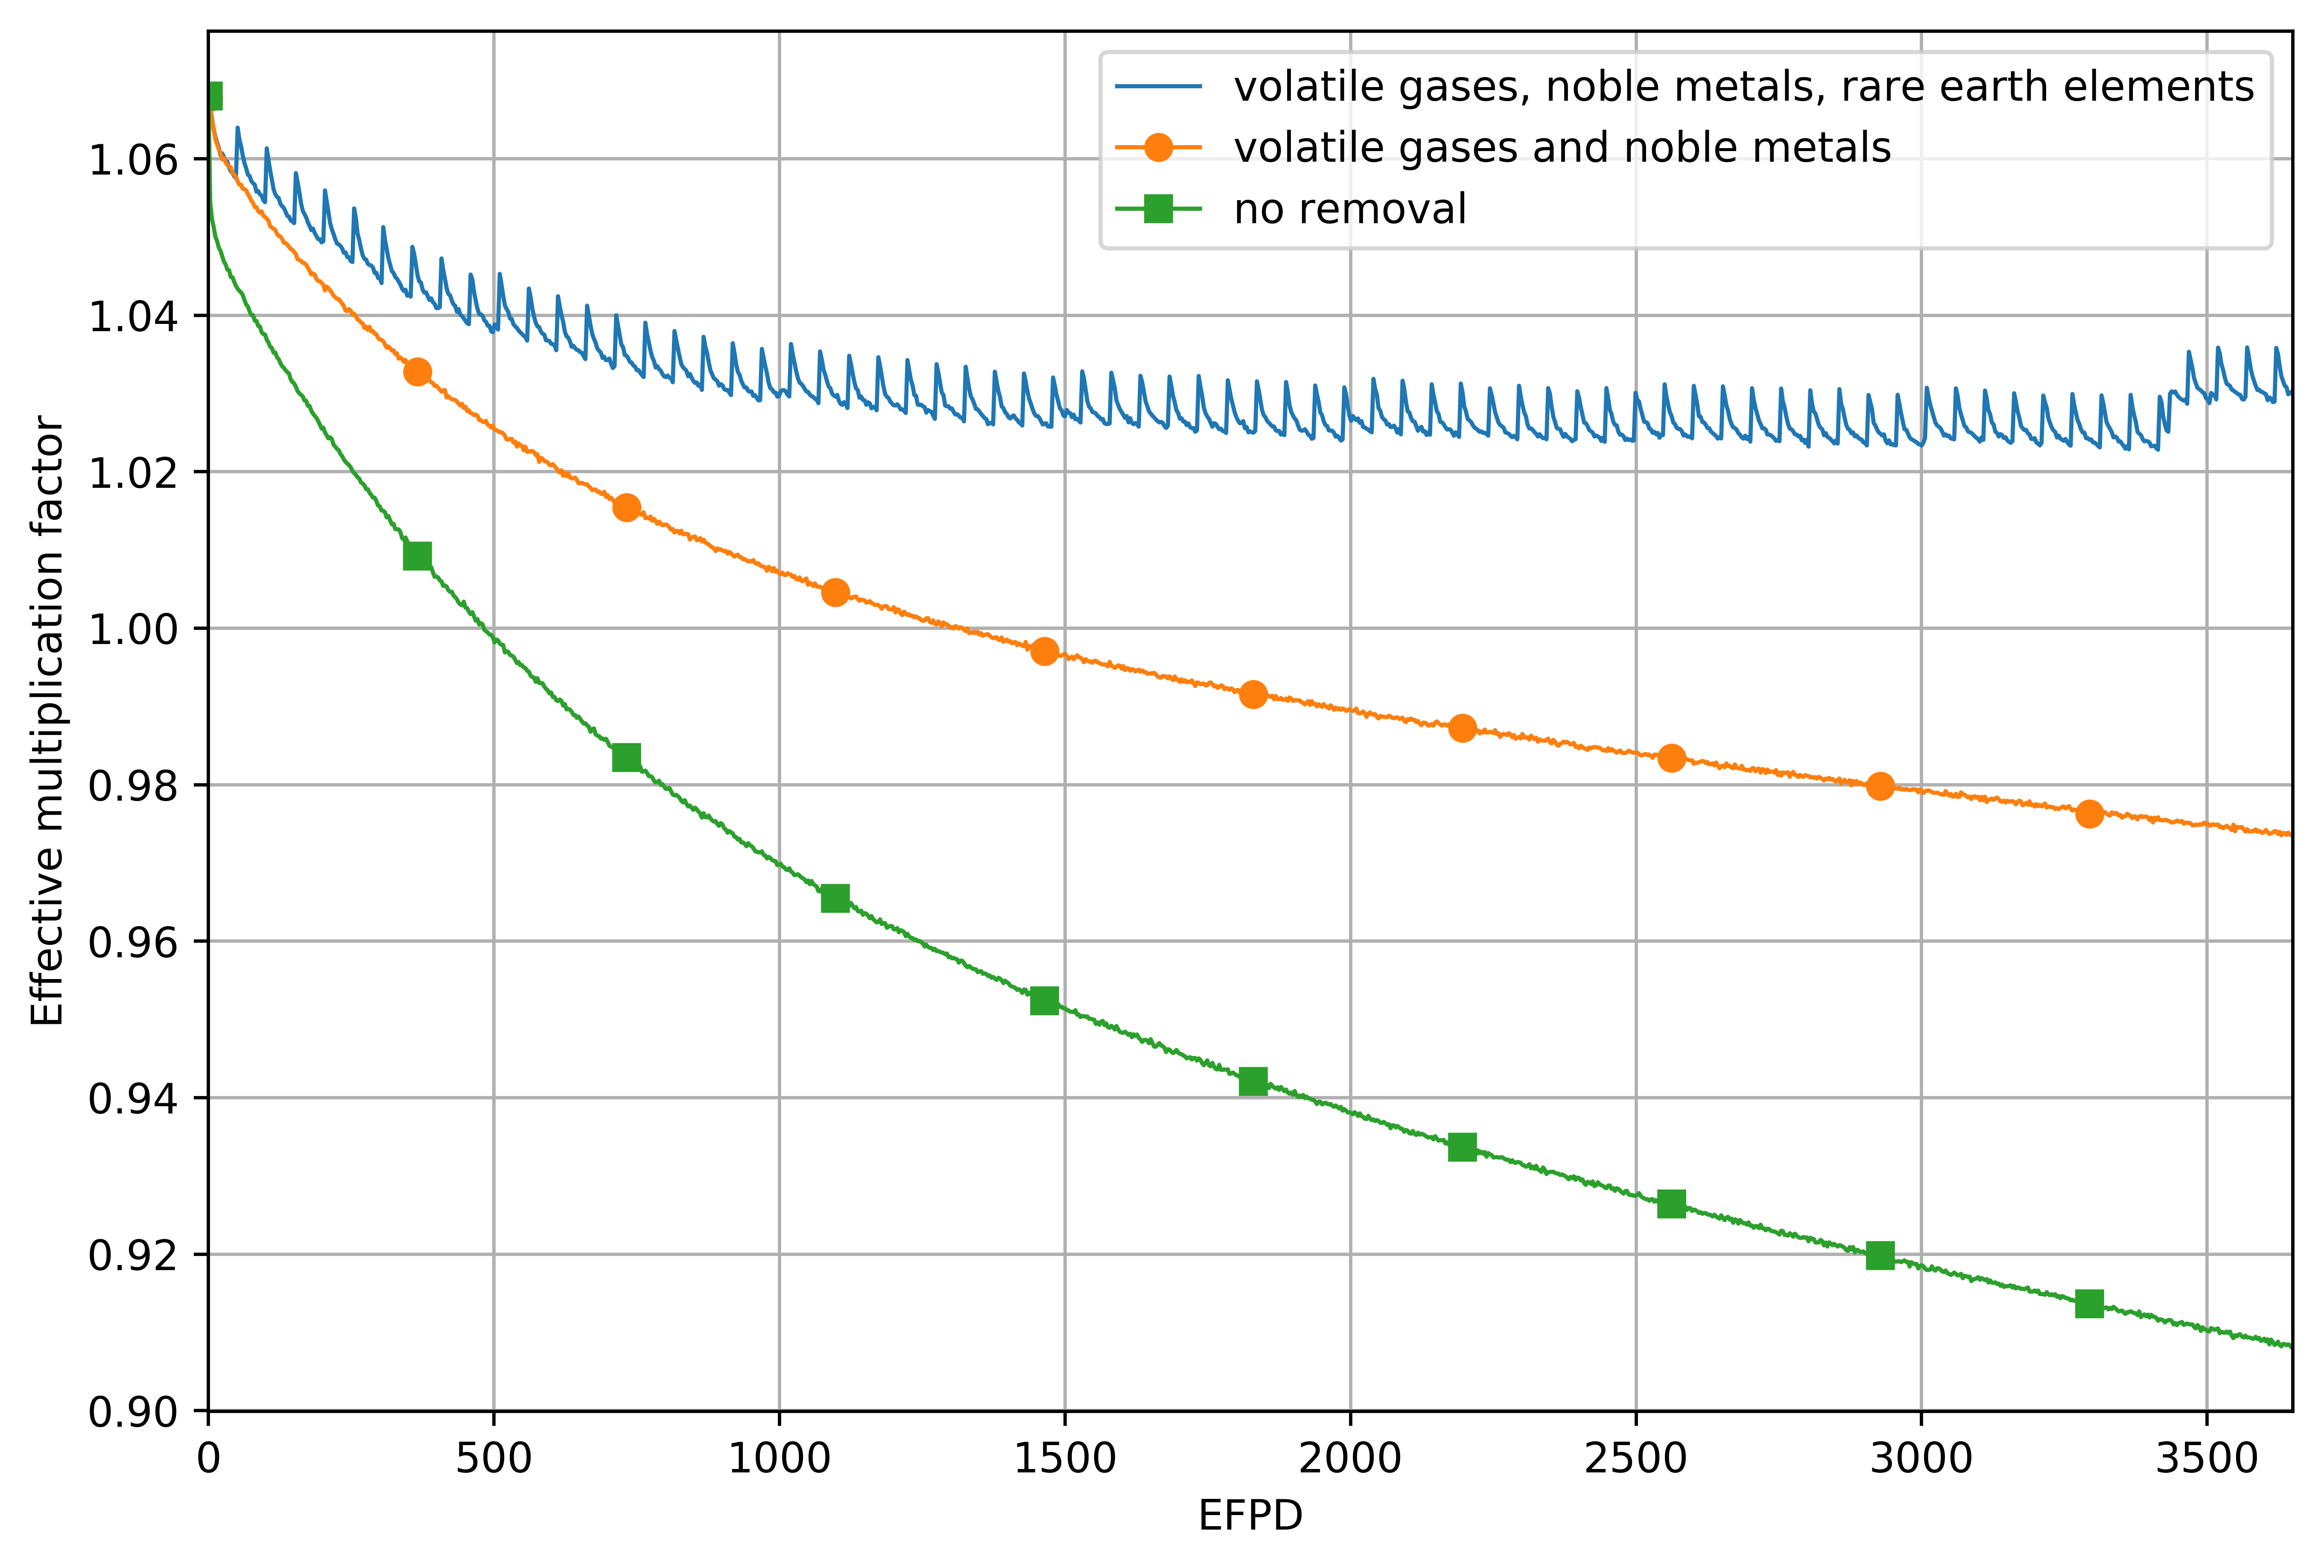
\includegraphics[width=\textwidth]{keff_rem_cases.png} 
  \caption{Calculated effective multiplication factor for full-core \gls{MSBR} 
model with removal of various fission product groups over 10 years of 
operation.}
  \label{fig:fp_removal}
\end{figure}

%\FloatBarrier
%\section{Discussion}
% This should explore the significance of the results of the work, not repeat
% them. A combined Results and Discussion section is often appropriate. Avoid
% extensive citations and discussion of published literature.
Short 2-3 paragraph discussion. This will emphasize:
\begin{itemize}
  \item Discuss reason of spectral shift (heavy \gls{FP} accumulation, Pu isotopes).
  \item Neutron spectral shift which causes safety parameters worsening.  
  \item Couple words about power profile.
\end{itemize}

%\FloatBarrier
%\section{Discussion and conclusions}

This work introduces the open source \gls{MSR} simulation package SaltProc. 
SaltProc expands the capability of SERPENT2, the continuous-energy Monte Carlo 
code to include online reprocessing modeling capabilities 
\cite{rykhlevskii_arfc/saltproc:_2018}. Benefits of SaltProc include 
generic geometry modeling, multi-flow capabilities, time-dependent feed and 
removal rates, and the ability to specify removal efficiency. The main goal of 
this work has 
been to demonstrate SaltProc's capability to find the equilibrium fuel salt 
composition (where equilibrium is defined as when the number densities of major 
isotopes vary by less than 1\% over several years). A secondary goal has been to 
compare predicted operational and safety parameters (e.g., neutron energy 
spectrum, power and breeding distribution, temperature coefficients of 
reactivity) of the \gls{MSBR} at startup and equilibrium state. A tertiary goal 
has been to demonstrate benefits of continuous fission products removal for 
thermal \gls{MSR} design.

To achieve these goals, a full-core high-fidelity benchmark model of the \gls{MSBR} 
was implemented in SERPENT2. The full-core model was used instead of the 
the simplified single-cell model \cite{betzler_molten_2017, 
rykhlevskii_online_2017, betzler_fuel_2018} to precisely describe the 
two-region \gls{MSBR} concept design sufficiently to accurately represent 
breeding in the outer core zone. When running depletion calculations, the most 
important fission products and $^{233}$Pa are removed while fertile and fissile 
materials are added to the fuel salt every 3 days.  Meanwhile, the removal 
interval for the rare earths, volatile fluorides, and seminoble metals was greater 
than month a (50 days), which caused effective multiplication factor fluctuation. 

\subsection{Equilibrium state search}
The results of this study indicate that the effective multiplication factor 
slowly decreases from 1.075 and reaches 1.02 at equilibrium after approximately 
6 years of operation. At the same time, the concentrations of $^{233}$U, $^{232}$Th, 
$^{233}$Pa, $^{232}$Pa stabilized after approximately 2500 days of operation. 
Particularly, $^{233}$U number density equilibrates\footnote{fluctuates less 
than 0.8\%} after 16 years of operation. Consequently, the core reaches the quasi-equilibrium state after 16 years of operation. However, a wide variety of nuclides, 
including fissile isotopes (e.g. $^{233}$U, $^{239}$Pu) and non-fissile strong 
absorbers (e.g. $^{234}$U), continue accumulating in the core. 

\subsection{Spectral shift}
We also found that the neutron energy spectrum grew harder as the core  
approaches equilibrium because significant heavy fission products accumulated in 
the \gls{MSBR} core. Moreover, the neutron energy spectrum in the central core 
region is much softer than in the outer core region due to lower 
moderator-to-fuel ratio in the outer zone, and this distribution remains stable 
during reactor operation. Finally, the epithermal or thermal spectrum is needed 
to effectively breed $^{233}$U from $^{232}$Th because radiative capture cross 
section of thorium-232 monotonically decreases from $10^{-10}$ MeV to $10^{-5}$ 
MeV. A harder spectrum in the outer core region tends to significantly increase 
resonance absorption in thorium and decrease the absorptions in fissile and 
structural materials. 

The spatial power distribution in the \gls{MSBR} shows that 98\% of the fission 
power is generated in central zone I, and neutron energy spectral shift did not 
cause any notable changes in a power distribution. The spatial distribution of 
neutron capture reaction rate for fertile $^{232}$Th, corresponding to breeding in 
the core, confirms that most of the breeding occurs in an outer, 
undermoderated, region of the \gls{MSBR} core. Finally, the average $^{232}$Th 
refill rate throughout 60 years of operation is approximately 2.40 kg/day or 
100 g/GWh$_e$.

We compared the safety parameters for the initial fuel loading and 
equilibrium compositions using the SERPENT2 Monte Carlo code. 
The total temperature coefficient 
is large and negative at startup and equilibrium but the magnitude decreases 
throughout reactor operation from $-3.10$ to $-0.94$ pcm/K as the spectrum 
hardens. The moderator 
temperature coefficient is positive and also decreases during fuel depletion. 
The reactivity control system efficiency analysis showed that the safety rod integral 
worth decreases by approximately 16.2\% over 16 years of operation, while 
graphite rod integral worth remains constant. Therefore, neutron energy 
spectrum hardening during fuel salt depletion has an undesirable impact on 
\gls{MSBR} stability and controllability, and should be taken into 
consideration in further analysis of transient accident scenarios.

\subsection{Benefits of fission product removal}

The \gls{MSBR} core performance benefits from the removal of volatile gases, 
noble metals, and rare earths from the fuel salt. 
Moreover, immediate removal of volatile gases (e.g., xenon) and noble metals 
increased reactivity by approximately 7500 pcm over a 10-year 
timeframe. In contrast, the effect of relatively slower removal of rare earth 
elements (every 50 days cycle instead of 3 days) has less impact (5500 pcm) on 
the core reactivity after 10 years of operation. An additional study 
is needed to establish neutronic  and economic tradeoffs of removing each element.

\subsection{Future work}
SaltProc-SERPENT coupled simulation efforts could progress in a 
number of different directions. First optimization of reprocessing parameters (e.g. time step, feeding rate, 
protactinium removal rate) could establish the best fuel utilization, breeding 
ratio, or safety characteristics for various designs. This might be performed with a parameter sweeping 
outer loop which would change an input parameter by a small increment, run the 
simulation and analyze output to determine optimal configuration. Alternatively, 
the existing RAVEN optimization framework \cite{alfonsi_raven_2013} might be 
employed for such optimization studies.

Only the batch-wise online reprocessing approach has been treated in this 
work. However, the SERPENT2 Monte Carlo code was extended for 
continuous online fuel reprocessing simulation \cite{aufiero_extended_2013}. 
This extension must be verified against existing SaltProc/SERPENT or 
ChemTriton/SCALE packages, and could be employed for immediate removal of 
fission product gases (e.g., Xe, Kr) which have a strong negative impact on 
core lifetime and breeding efficiency. Finally, using the built-in SERPENT2 
Monte Carlo code online reprocessing \& refueling material burnup routine would 
significantly speed up computer-intensive full-core depletion simulations.

%\FloatBarrier
%\section{Acknowledgments}

This research is part of the Blue Waters sustained-petascale computing project, 
which is supported by the National Science Foundation (awards OCI-0725070 and 
ACI-1238993) and the state of Illinois. Blue Waters is a joint effort of the 
University of Illinois at Urbana-Champaign and its National Center for 
Supercomputing Applications 

The authors would like to thank  members of the \gls{ARFC} group at the 
University of Illinois - Urbana Champaign who provided valuable code reviews 
and proofreading.

The authors contributed to this work as described below.  Andrei Rykhlevskii 
conceived and designed the simulations, wrote the paper, prepared figures 
and/or tables, performed the computation work, contributed to the software 
product, and reviewed drafts of the paper. Jin Whan Bae conceived and designed 
the simulations, wrote the paper, contributed to the software 
product, and reviewed drafts of the paper. Andrei Rykhlevskii 
is supported by 
DOE ARPA-E MEITNER program award 1798-1576. 
Jin Whan
Bae is supported by funding received from the DOE Nuclear Energy University
Program (Project 16-10512) `Demand-Driven Cycamore Archetypes'.

Kathryn D. Huff directed and 
supervised the work, conceived and designed the simulations, 
contributed to the software product, and reviewed drafts of the paper.  Prof. 
Huff is supported by the Nuclear Regulatory Commission Faculty Development 
Program, the National Center for Supercomputing Applications, the NNSA Office 
of Defense Nuclear Nonproliferation R\&D through the Consortium for Verfication 
Technologies and the Consortium for Nonproliferation Enabling Capabilities,  
the International Institute for Carbon Neutral Energy Research (WPI-I2CNER), 
sponsored by the Japanese Ministry of Education, Culture, Sports, Science and 
Technology, and DOE ARPA-E MEITNER program award 1798-1576. 


%\FloatBarrier

%\nocite{robertson_conceptual_1971} % placeholder until citations appear
\bibliography{../dissertation/thesisrefs}

\end{document}
